% DIICSU Honours Project LaTeX Template


\documentclass[12pt,a4paper]{article}
\usepackage{geometry}
\usepackage{mathptmx}  % Times New Roman style font
\usepackage{setspace}
\usepackage{titlesec}
\usepackage{titletoc}
\usepackage{tocloft}
\usepackage{graphicx}
\usepackage{caption}
\usepackage{subcaption}
\usepackage{float}
\usepackage{amsmath}
\usepackage{amssymb}
\usepackage{booktabs}
\usepackage{hyperref}
\usepackage[style=ieee]{biblatex}
\addbibresource{sample.bib}
\usepackage{listings}
\usepackage{xcolor}
\usepackage{appendix}
\usepackage{pdfpages}
\usepackage{fancyhdr}
\usepackage{enumitem}
\usepackage{multirow}
\usepackage{array}

% Graphics path
\graphicspath{{media/}}

% Page layout
\geometry{
    left=1in,
    right=1in,
    top=1in,
    bottom=1in,
    includeheadfoot
}

% Single spacing (as per requirements)
\singlespacing

% Set font size to 12pt
\renewcommand{\normalsize}{\fontsize{12}{14}\selectfont}

% Title formatting
\titleformat{\section}
    {\normalfont\Large\bfseries}{\thesection}{1em}{}
\titleformat{\subsection}
    {\normalfont\large\bfseries}{\thesubsection}{1em}{}
\titleformat{\subsubsection}
    {\normalfont\normalsize\bfseries}{\thesubsubsection}{1em}{}
\titleformat{\paragraph}
    {\normalfont\normalsize\itshape}{\theparagraph}{1em}{}

% Table of Contents formatting
\renewcommand{\cftsecleader}{\cftdotfill{\cftdotsep}}
\renewcommand{\contentsname}{Table of Contents}
\setcounter{tocdepth}{3}

% Header and footer
\pagestyle{fancy}
\fancyhf{}
\fancyhead[R]{\thepage}
\renewcommand{\headrulewidth}{0pt}

% Caption formatting
\captionsetup{labelfont=bf, justification=raggedright, singlelinecheck=false}

% Code listing style
\lstset{
    basicstyle=\ttfamily\small,
    breaklines=true,
    frame=single,
    numbers=left,
    numberstyle=\tiny,
    tabsize=4,
    showstringspaces=false,
    keywordstyle=\color{blue},
    commentstyle=\color{gray},
    stringstyle=\color{red}
}

% Hyperlink setup
\hypersetup{
    colorlinks=true,
    linkcolor=blue,
    citecolor=blue,
    filecolor=blue,
    urlcolor=blue,
    pdftitle={Adversarial Robustness of Medical Image Classification},
    pdfauthor={Ruifeng Yan}
}

% Custom commands
\newcommand{\projecttitle}{Evaluating Adversarial Robustness of Deep Learning Models for Medical Chest X-ray Classification}
\newcommand{\studentname}{Ruifeng Yan}
\newcommand{\studentid}{2542795}
\newcommand{\supervisor}{Perley Xu}

% Abstract environment
\renewenvironment{abstract}
    {\small
    \begin{center}
    \textbf{Abstract}
    \end{center}
    \quotation}
    {\endquotation}

% Acknowledgements section
\newcommand{\acknowledgments}[1]{
    \phantomsection
    \section*{Acknowledgments}
    \addcontentsline{toc}{section}{Acknowledgments}
    #1
}

% Appendix setup
\renewcommand{\appendixname}{Appendices}
\renewcommand{\appendixtocname}{Appendices}

\begin{document}

% Title page
\begin{titlepage}
    \centering
    \vspace*{2cm}
    
    {\LARGE\textbf{\projecttitle}}\\
    \vspace{1cm}
    
    {\Large \studentname}\\
    \vspace{0.5cm}
    
    {\Large \studentid}\\
    \vspace{1cm}
    
    {\LARGE\textbf{DI40001 DIICSU Honours Project}}\\
    \vspace{1cm}
    
    {\Large Supervisor: \supervisor}\\
    \vspace{2cm}
    
    \vfill
    \today
\end{titlepage}

% Abstract page
\begin{abstract}
Deep learning models have achieved remarkable success in medical image classification, particularly in chest X-ray analysis for disease detection. However, the vulnerability of these models to adversarial attacks poses significant concerns for clinical deployment where diagnostic accuracy directly impacts patient outcomes. This project presents a comprehensive evaluation of adversarial robustness for a ResNet-18 based chest X-ray classification model trained on the NIH ChestX-ray14 dataset. We systematically investigate model vulnerability under two prominent adversarial attack methods: Fast Gradient Sign Method (FGSM) and Projected Gradient Descent (PGD), analyzing performance degradation across multiple perturbation magnitudes ranging from $\epsilon=0.25/255$ to $\epsilon=2/255$. Our baseline model achieves 68.51\% accuracy and 0.704 AUC on clean test data comprising 25,583 images. Under adversarial perturbations, we observe severe performance degradation, with FGSM reducing accuracy to 2.80\% and PGD to 0.08\% at $\epsilon=2/255$. Through extensive visualization using Gradient-weighted Class Activation Mapping (Grad-CAM), we demonstrate how adversarial perturbations fundamentally alter the model's attention patterns and decision-making process. Our findings highlight the critical need for robust defense mechanisms before deploying deep learning systems in clinical settings, and provide a systematic framework for evaluating medical AI robustness.

\textbf{Keywords:} Adversarial robustness, Medical image classification, Chest X-ray, Deep learning, FGSM, PGD, Grad-CAM, Neural network security
\end{abstract}

\newpage

% Table of Contents
\tableofcontents
\newpage

% Acknowledgments
\acknowledgments{
\hspace{2em}I would like to express my sincere gratitude to my supervisor for her invaluable guidance and support throughout this project. Her expertise in machine learning and medical imaging provided essential direction for this research.

I am also grateful to the NIH Clinical Center for making the ChestX-ray14 dataset publicly available, which enabled this research on adversarial robustness in medical imaging.

Additionally, I thank the open-source community for developing and maintaining the tools and libraries that made this work possible, including PyTorch, NumPy, Matplotlib, and scikit-learn.

Finally, I would like to express my heartfelt thanks to all the teachers, family members, and friends who have accompanied me through my four years of university. Special thanks to my girlfriend for her unwavering support and encouragement throughout this journey.
}

\newpage

%==============================================================================
% SECTION 1: INTRODUCTION
%==============================================================================
\section{Introduction}
\label{sec:introduction}

\subsection{Background and Motivation}

The integration of artificial intelligence into healthcare has transformed medical diagnostics, with deep learning models demonstrating remarkable capabilities in analyzing medical images. Chest X-ray interpretation, one of the most common radiological examinations performed worldwide with over 2 billion procedures annually, has particularly benefited from these advances \cite{rajpurkar2017}. Automated systems can now assist radiologists in detecting various thoracic conditions including pneumonia, tuberculosis, lung nodules, cardiomegaly, and pleural effusion with accuracy approaching or exceeding human experts in certain controlled tasks.

The COVID-19 pandemic further accelerated the adoption of AI-based diagnostic tools, with numerous studies demonstrating the potential of deep learning models to identify COVID-19 related pulmonary abnormalities from chest radiographs \cite{roberts2021}. Healthcare institutions worldwide have begun exploring the deployment of these systems to augment clinical workflows, reduce diagnostic delays, improve patient outcomes in resource-limited settings, and address the global shortage of trained radiologists.

Deep learning has revolutionized medical image analysis through its ability to automatically learn hierarchical feature representations from large datasets. Convolutional neural networks (CNNs), in particular, have proven exceptionally effective at capturing spatial patterns in medical images that correlate with pathological findings. The release of large-scale annotated datasets such as the NIH ChestX-ray14 \cite{wang2017}, CheXpert \cite{irvin2019}, and MIMIC-CXR \cite{johnson2019} has been instrumental in enabling the development and validation of increasingly sophisticated deep learning approaches.

However, this rapid adoption raises critical concerns about the reliability and safety of these AI systems. Unlike traditional software systems where behavior is deterministic and well-understood, deep neural networks operate as complex nonlinear functions with millions of parameters, making their decision boundaries difficult to characterize. This opacity becomes particularly concerning when considering the potential for adversarial manipulation, which could have life-threatening consequences in medical settings.

\subsection{The Adversarial Threat}

Adversarial examples represent carefully crafted perturbations that, while imperceptible or nearly imperceptible to human observers, can cause neural networks to produce dramatically incorrect outputs with high confidence \cite{szegedy2014}. Since their discovery in the context of image classification, adversarial examples have been demonstrated across virtually every domain where deep learning is applied, including natural language processing, speech recognition, autonomous driving, and critically, medical imaging.

The phenomenon of adversarial vulnerability challenges fundamental assumptions about deep learning generalization. Standard theory suggests that models achieving low error on test data have learned meaningful representations of the underlying data distribution. However, adversarial examples demonstrate that the learned decision boundaries can be highly irregular, with correctly classified points surrounded by vast regions of incorrectly classified inputs. This brittleness suggests that current deep learning models may rely on superficial statistical correlations rather than semantically meaningful features.

The implications for healthcare are profound: an adversarial attack could potentially cause a diagnostic AI system to miss a critical finding such as a tumor or pneumonia, or conversely, generate false positive diagnoses leading to unnecessary interventions. Either outcome could result in direct patient harm, making adversarial robustness a critical consideration for clinical deployment.

Several factors make medical imaging particularly vulnerable to adversarial manipulation. First, medical images traverse complex digital pathways from acquisition through interpretation, including Picture Archiving and Communication Systems (PACS), cloud storage, telemedicine transmission, and display devices, each presenting potential points of attack. Second, the high resolution and information density of medical images provides attackers with enormous flexibility in crafting perturbations. Third, the subtle nature of many pathological findings means that adversarial perturbations can easily mask or mimic disease patterns.

\subsection{Problem Statement}

Despite significant advances in medical image classification and growing awareness of adversarial threats, the robustness of medical AI systems remains poorly understood and inadequately addressed. Several factors contribute to this critical gap:

First, the unique characteristics of medical images, including their grayscale nature, specific anatomical structures, standardized acquisition protocols, and subtle pathological features, create distinct challenges compared to natural image classification tasks. Adversarial perturbations that exploit these characteristics may behave differently than those targeting general-purpose image classifiers trained on datasets like ImageNet.

Second, the clinical deployment context introduces additional considerations for threat modeling. Unlike general computer vision applications where adversarial robustness may be a secondary concern, medical AI systems operate in high-stakes environments where incorrect predictions can directly impact patient outcomes. The acceptable level of robustness must be calibrated to these consequences.

Third, systematic robustness evaluation methodologies for medical imaging remain underdeveloped. While the adversarial machine learning community has established standard benchmarks and evaluation protocols for natural image classification, corresponding frameworks for medical imaging are limited. This hampers the ability to compare different models and defense mechanisms in a principled manner.

This project addresses the fundamental question: \textit{How vulnerable are deep learning models for chest X-ray classification to adversarial perturbations, and what insights can systematic robustness evaluation provide for improving clinical AI safety?}

\subsection{Research Objectives}

This project pursues the following specific objectives:

\begin{enumerate}[leftmargin=*]
    \item \textbf{Develop a comprehensive evaluation framework:} Design and implement a systematic methodology for assessing adversarial robustness in medical image classification, incorporating multiple attack methods, perturbation magnitudes, and evaluation metrics relevant to clinical deployment.
    
    \item \textbf{Train a baseline classification model:} Develop a ResNet-18 based chest X-ray classification model using the NIH ChestX-ray14 dataset, establishing baseline performance metrics for subsequent robustness evaluation.
    
    \item \textbf{Quantify vulnerability under gradient-based attacks:} Measure the performance degradation of the chest X-ray classification model under FGSM and PGD attacks across a range of perturbation budgets, establishing benchmark robustness metrics.
    
    \item \textbf{Analyze attack mechanisms through visualization:} Employ Grad-CAM and other interpretability techniques to understand how adversarial perturbations affect model attention patterns and feature representations, providing insights into attack mechanisms specific to medical imaging.
    
    \item \textbf{Compare attack effectiveness:} Systematically compare the effectiveness of single-step (FGSM) versus iterative (PGD) attacks, characterizing the relationship between attack sophistication and model vulnerability.
    
    \item \textbf{Establish reproducible benchmarks:} Create well-documented, reproducible evaluation protocols and open-source implementations that can serve as references for future research on medical imaging adversarial robustness.
\end{enumerate}

\subsection{Contributions}

This project makes the following contributions to the field of medical AI safety:

\begin{itemize}[leftmargin=*]
    \item A comprehensive empirical study of adversarial vulnerability in chest X-ray classification, providing detailed quantitative analysis across multiple attack types and perturbation magnitudes with a test set of over 25,000 images.
    
    \item An integrated evaluation framework combining accuracy metrics, calibration analysis (Expected Calibration Error), and visual interpretability (Grad-CAM) for holistic robustness assessment.
    
    \item Extensive visualization analysis demonstrating how adversarial perturbations alter model behavior at the feature level, providing insights into attack mechanisms specific to medical imaging.
    
    \item Open-source implementation of all evaluation tools, attack methods, and visualization techniques, enabling reproducibility and extension of this research by the broader community.
    
    \item Quantitative comparison of FGSM and PGD attacks demonstrating the significantly higher effectiveness of iterative attacks, with implications for defense prioritization.
\end{itemize}

\subsection{Report Structure}

The remainder of this report is organized as follows:

\textbf{Section 2: Literature Review} provides comprehensive background on deep learning for medical imaging, adversarial machine learning, and interpretability techniques, situating this work within the broader research context.

\textbf{Section 3: Methodology} describes the dataset, model architecture, adversarial attack methods, evaluation metrics, and visualization techniques employed in this study.

\textbf{Section 4: Implementation} details the technical implementation including the software architecture, training procedures, attack implementations, and evaluation pipeline.

\textbf{Section 5: Results and Discussion} presents experimental findings with detailed analysis of model vulnerability, attack effectiveness, and visualization insights.

\textbf{Section 6: Conclusions and Future Work} summarizes key findings, discusses limitations, and outlines directions for future research.

%==============================================================================
% SECTION 2: LITERATURE REVIEW
%==============================================================================
\section{Literature Review}
\label{sec:literature-review}

\subsection{Deep Learning for Medical Image Classification}

Deep learning has fundamentally transformed medical image analysis over the past decade, achieving state-of-the-art performance across numerous diagnostic tasks including dermatology, ophthalmology, pathology, and radiology \cite{litjens2017}. This transformation has been enabled by three key developments: the availability of large annotated datasets, advances in neural network architectures, and the computational power provided by modern GPUs.

The impact of deep learning on medical imaging extends beyond mere performance improvements. Traditional computer-aided diagnosis (CAD) systems relied on handcrafted features designed by domain experts, such as texture descriptors, shape features, and intensity histograms. These systems required extensive feature engineering and often failed to generalize across different imaging modalities, equipment manufacturers, or patient populations. Deep learning fundamentally changed this paradigm by enabling end-to-end learning, where the model automatically discovers relevant features directly from raw pixel data.

The potential clinical impact of accurate automated diagnosis is substantial. Radiology departments worldwide face increasing workloads as imaging becomes more accessible and prevalent in clinical practice. In many countries, there are significant shortages of trained radiologists, leading to diagnostic delays that can affect patient outcomes. Automated systems that can accurately triage or pre-screen medical images could help address these challenges, prioritizing urgent cases and reducing the burden on human experts.

\subsubsection{Convolutional Neural Networks}

Convolutional neural networks form the backbone of modern medical image analysis systems. The key innovation of CNNs is the use of learned convolutional filters that automatically extract hierarchical features from images, eliminating the need for manual feature engineering that characterized earlier approaches.

The architecture of CNNs is inspired by the organization of the visual cortex in biological systems. Early layers learn to detect low-level features such as edges, corners, and textures, while deeper layers combine these primitive features into increasingly complex and abstract representations. This hierarchical feature learning is particularly well-suited to medical imaging, where diagnostic patterns often involve combinations of texture, shape, and spatial relationships that are difficult to specify manually.

The fundamental operations in CNNs include convolution, pooling, and nonlinear activation. Convolution applies learnable filters across the input image, producing feature maps that highlight specific patterns. Pooling operations reduce spatial dimensions while retaining important information, providing translation invariance and reducing computational requirements. Nonlinear activation functions, such as ReLU (Rectified Linear Unit), introduce the nonlinearity necessary for learning complex decision boundaries.

The introduction of deeper networks with skip connections, particularly ResNet \cite{he2016}, addressed the vanishing gradient problem that had limited earlier deep architectures. The vanishing gradient problem occurs when gradients become extremely small during backpropagation through many layers, preventing effective learning in early layers. By enabling gradients to flow directly through skip connections, ResNet allowed training of networks with hundreds of layers while maintaining trainability. The skip connections create ``shortcut'' paths that allow gradients to bypass layers, ensuring that meaningful gradient signals reach all parts of the network during training.

ResNet-18, the architecture employed in this project, consists of 18 layers organized into residual blocks, providing an effective balance between model capacity and computational efficiency. Each residual block contains two convolutional layers with batch normalization and ReLU activation. The skip connection adds the input of the block directly to its output, allowing the network to learn residual mappings rather than direct mappings. This residual learning formulation has been shown to facilitate optimization and enable training of much deeper networks than previously possible.

The mathematical formulation of a residual block can be expressed as:
\begin{equation}
    \mathbf{y} = \mathcal{F}(\mathbf{x}, \{W_i\}) + \mathbf{x}
\end{equation}
where $\mathbf{x}$ is the input, $\mathbf{y}$ is the output, and $\mathcal{F}$ represents the residual mapping to be learned. The addition operation requires that $\mathbf{x}$ and $\mathcal{F}$ have the same dimensions; when this is not the case, a linear projection is applied to match dimensions.

DenseNet \cite{huang2017} further improved on this approach by connecting each layer to every other layer in a feed-forward fashion. Rather than adding the input to the output as in ResNet, DenseNet concatenates feature maps from all preceding layers, creating dense connections throughout the network. This dense connectivity pattern encourages feature reuse, reduces the number of parameters, and strengthens gradient propagation. Each layer receives ``collective knowledge'' from all preceding layers, leading to more efficient feature utilization.

The DenseNet-121 architecture has become particularly popular for chest X-ray classification following its use in CheXNet \cite{rajpurkar2017}. The architecture consists of four dense blocks separated by transition layers that perform downsampling. Within each dense block, layers are densely connected with a growth rate parameter controlling the number of new feature maps added by each layer. This architecture achieves competitive performance with fewer parameters than comparable ResNet models.

Other notable architectures that have been applied to medical imaging include VGGNet, which demonstrated the importance of depth using small (3x3) convolutional filters; Inception networks, which use parallel convolutional paths with different filter sizes; and EfficientNet, which systematically scales network width, depth, and resolution. Each architecture offers different trade-offs between accuracy, computational cost, and memory requirements, and the optimal choice depends on the specific application and available resources.

\subsubsection{Transfer Learning in Medical Imaging}

Transfer learning, the practice of initializing networks with weights pre-trained on large datasets, has proven remarkably effective for medical imaging despite the significant domain gap between natural images and medical scans \cite{raghu2019}. Models pre-trained on ImageNet learn low-level features such as edges, textures, and shapes that transfer well across domains, while higher-level features are adapted through fine-tuning on the target medical dataset.

The theoretical foundation for transfer learning rests on the observation that neural networks learn hierarchical representations, with early layers capturing generic, task-independent features and later layers learning task-specific representations. In the context of image classification, early convolutional layers learn to detect edges, textures, and simple patterns that are relevant across virtually all image domains. These generic features can be directly reused for medical imaging tasks, while only the higher-level, task-specific layers require adaptation.

Research has shown that ImageNet pre-training provides significant benefits even when the source and target domains differ substantially. Raghu et al. \cite{raghu2019} found that transfer learning consistently improves performance in medical imaging, though the optimal strategy depends on the size of the target dataset and the similarity between domains. For small medical datasets, pre-training provides substantial regularization that prevents overfitting. The pre-trained weights serve as a strong prior that constrains the solution space, preventing the model from memorizing noise in limited training data.

Several transfer learning strategies have been explored in medical imaging. The simplest approach, feature extraction, freezes all pre-trained layers and only trains a new classification head. Fine-tuning involves unfreezing some or all pre-trained layers and training them with a small learning rate to adapt to the new domain. More sophisticated approaches include gradual unfreezing, where layers are progressively unfrozen during training, and discriminative learning rates, where different learning rates are applied to different layers.

The choice between these strategies depends on several factors. When the target dataset is small and the domain gap is large, aggressive fine-tuning may lead to overfitting, making feature extraction preferable. When the target dataset is large, full fine-tuning typically yields the best results. The similarity between source and target domains also matters: medical images differ substantially from ImageNet in color characteristics (often grayscale), content (anatomical structures vs. natural objects), and texture patterns, suggesting that substantial adaptation may be beneficial.

Recent work has also explored alternative pre-training strategies specifically designed for medical imaging. Self-supervised pre-training on large collections of unlabeled medical images can learn domain-specific representations that may transfer better to downstream tasks. Contrastive learning approaches, such as SimCLR and MoCo, have shown promising results in this direction. However, ImageNet pre-training remains a strong baseline that is difficult to surpass without very large amounts of domain-specific data.

\subsubsection{Chest X-ray Classification}

The NIH ChestX-ray14 dataset, introduced by Wang et al. \cite{wang2017}, represented a landmark contribution to chest X-ray analysis research. Comprising over 112,000 frontal-view chest X-rays from more than 30,000 patients, with 14 disease labels extracted from radiological reports using natural language processing, it enabled the first large-scale deep learning studies of thoracic pathology detection.

The 14 disease categories in ChestX-ray14 include Atelectasis, Cardiomegaly, Effusion, Infiltration, Mass, Nodule, Pneumonia, Pneumothorax, Consolidation, Edema, Emphysema, Fibrosis, Pleural Thickening, and Hernia. These conditions span a range of thoracic pathologies with varying prevalence, severity, and clinical significance. Many images contain multiple conditions, making this a multi-label classification problem in its full formulation.

CheXNet, developed by Rajpurkar et al. \cite{rajpurkar2017}, demonstrated that a DenseNet-121 model trained on ChestX-ray14 could achieve radiologist-level performance in pneumonia detection, generating significant excitement about AI-assisted diagnosis. The study compared model performance against the consensus of four radiologists, finding that the model achieved an AUC of 0.768 on pneumonia detection, exceeding the average radiologist performance of 0.633. This result suggested that deep learning could potentially augment or even replace human experts in certain diagnostic tasks.

Subsequent work has addressed multi-label classification, uncertainty quantification, and domain adaptation challenges in chest X-ray analysis. The CheXpert dataset, released by Irvin et al. \cite{irvin2019}, introduced uncertainty labels to handle cases where radiological reports express uncertainty about findings. MIMIC-CXR, the largest publicly available chest X-ray dataset with over 370,000 images, has enabled studies of model generalization and multi-site validation. These datasets have collectively advanced the field toward more robust and clinically applicable models.

However, the field has also recognized important limitations. Label quality in ChestX-ray14, derived through automated text mining rather than expert annotation, introduces noise that can affect model training and evaluation. Studies have found significant disagreement between NLP-extracted labels and expert annotations for certain conditions, particularly those requiring subtle interpretation of radiological findings. This label noise can limit model performance and complicate evaluation.

Additionally, models trained on single-institution data may not generalize well across different imaging equipment, patient populations, and clinical protocols. Domain shift, where the distribution of test data differs from training data, is a pervasive challenge in medical imaging. Factors contributing to domain shift include differences in X-ray equipment manufacturers, acquisition parameters, patient positioning, and demographic characteristics. Models that perform well on one dataset may show significantly degraded performance when deployed at different institutions.

The clinical deployment of chest X-ray classification models raises additional considerations. Radiologists do not interpret images in isolation but consider patient history, clinical presentation, and other diagnostic information. Models trained purely on image data may miss important contextual information. Furthermore, the workflow integration of AI systems requires careful consideration of how automated predictions are presented to clinicians to maximize benefit while avoiding automation bias and over-reliance.

\subsubsection{Performance Metrics in Medical Image Classification}

Evaluating medical image classification models requires careful consideration of appropriate metrics that reflect clinical utility. Accuracy, while intuitive, can be misleading for imbalanced datasets where one class predominates. In chest X-ray classification, the prevalence of different conditions varies widely, making class-balanced metrics essential.

The Area Under the Receiver Operating Characteristic Curve (AUC-ROC) has become the standard metric for medical image classification. AUC-ROC measures the ability of a model to discriminate between positive and negative cases across all possible classification thresholds. A value of 0.5 indicates random performance, while 1.0 indicates perfect discrimination. AUC-ROC is threshold-independent and robust to class imbalance, making it suitable for comparing models across different datasets and conditions.

Sensitivity (recall) and specificity are particularly important in medical contexts. Sensitivity measures the proportion of true positive cases correctly identified, while specificity measures the proportion of true negative cases correctly identified. The appropriate trade-off between sensitivity and specificity depends on the clinical application. For screening applications where missing disease is more costly than false alarms, high sensitivity is prioritized. For confirmatory testing where false positives lead to unnecessary interventions, high specificity may be preferred.

Calibration, which measures how well predicted probabilities match observed frequencies, is increasingly recognized as important for clinical deployment. A well-calibrated model that predicts 70\% probability of disease should be correct approximately 70\% of the time. Miscalibrated models can lead to inappropriate clinical decisions if probabilities are interpreted literally. Expected Calibration Error (ECE) is a common metric for assessing calibration, measuring the weighted average discrepancy between predicted confidence and actual accuracy across probability bins.

\subsection{Adversarial Examples in Deep Learning}

\subsubsection{Discovery and Characterization}

Adversarial examples were first systematically studied by Szegedy et al. \cite{szegedy2014}, who made the surprising discovery that imperceptible perturbations to input images could cause state-of-the-art neural networks to misclassify with high confidence. This finding challenged assumptions about deep learning generalization and revealed that the learned decision boundaries are far more irregular than previously understood.

The discovery of adversarial examples was initially counterintuitive because it seemed to contradict the impressive generalization performance of deep neural networks. If models could correctly classify millions of test images that they had never seen during training, how could tiny perturbations cause catastrophic failures? The resolution of this apparent paradox lies in the geometry of high-dimensional spaces and the nature of learned decision boundaries.

The adversarial perturbations discovered by Szegedy et al. \cite{szegedy2014} exhibited several counterintuitive properties. First, they could be made arbitrarily small in magnitude while still causing misclassification. This implies that correctly classified examples often lie extremely close to decision boundaries, with adversarial examples existing in their immediate neighborhood. Second, the same perturbation often transferred across different model architectures, suggesting that adversarial vulnerability reflects fundamental properties of the data representation rather than artifacts of specific training procedures.

The transferability property has significant security implications. It means that an attacker can craft adversarial examples using a surrogate model and then use those examples to attack a different target model. This enables black-box attacks where the attacker has no direct access to the target model's parameters or gradients. Transferability has been observed across models trained on the same dataset, models trained on different datasets, and even models with different architectures.

Goodfellow et al. \cite{goodfellow2015} provided theoretical insight by proposing the ``linear hypothesis,'' suggesting that adversarial vulnerability arises from the linear behavior of neural networks in high-dimensional spaces. Even when individual activation functions are nonlinear, the cumulative effect of many small linear contributions can produce large changes in output for perturbations aligned with the model's gradient.

Consider a linear classifier with weights $\mathbf{w}$ applied to an input $\mathbf{x}$. Adding a perturbation $\boldsymbol{\eta}$ changes the output by $\mathbf{w}^T \boldsymbol{\eta}$. If the perturbation is constrained to have $L_\infty$ norm at most $\epsilon$, the maximum change in output is achieved when $\boldsymbol{\eta} = \epsilon \cdot \text{sign}(\mathbf{w})$, yielding a change of $\epsilon \cdot \|\mathbf{w}\|_1$. In high-dimensional spaces where the input has thousands or millions of dimensions (as in images), this sum can be very large even for small $\epsilon$, because the $L_1$ norm scales with dimensionality.

This linear explanation motivates the Fast Gradient Sign Method (FGSM) attack and suggests that adversarial vulnerability may be an inherent property of high-dimensional linear classifiers. However, neural networks are not purely linear, and subsequent research has shown that the full picture is more complex. Nonetheless, the linear hypothesis provides useful intuition and has guided the development of both attack and defense methods.

Alternative theories have been proposed to explain adversarial vulnerability. The ``tilted decision boundary'' hypothesis suggests that decision boundaries near training data are not perpendicular to the data manifold but are instead tilted, creating large regions of misclassified inputs nearby correctly classified ones. The ``feature hypothesis'' proposes that adversarial perturbations exploit non-robust features---patterns that are predictive on natural data but can be easily manipulated by small perturbations. Under this view, adversarial vulnerability reflects a fundamental trade-off between using all available predictive information (which improves accuracy) and using only robust features (which improves adversarial robustness).

Recent work has also connected adversarial vulnerability to properties of the data distribution and the training process. Models trained on limited data may learn decision boundaries that do not align with the true data manifold, creating adversarial vulnerabilities in regions where training data is sparse. Data augmentation and regularization techniques can partially address these issues by encouraging smoother decision boundaries, but they do not eliminate adversarial vulnerability.

\subsubsection{Attack Methods}

A taxonomy of adversarial attacks can be organized along several dimensions. White-box attacks assume the attacker has complete knowledge of the target model, including its architecture, parameters, and gradients. Black-box attacks assume limited or no knowledge of the target model, relying on query access or transferability from surrogate models. Targeted attacks aim to cause misclassification to a specific target class, while untargeted attacks simply aim to cause any misclassification. The perturbation budget may be measured in different norms, with $L_\infty$, $L_2$, and $L_0$ being most common.

The Fast Gradient Sign Method (FGSM), introduced by Goodfellow et al. \cite{goodfellow2015}, provides a computationally efficient single-step attack that remains widely used for robustness evaluation. FGSM computes the gradient of the loss function with respect to the input and applies a perturbation in the sign direction of this gradient:

\begin{equation}
    x_{adv} = x + \epsilon \cdot \text{sign}(\nabla_x \mathcal{L}(\theta, x, y))
\end{equation}

where $\mathcal{L}$ is the loss function, $\theta$ represents model parameters, $x$ is the input, $y$ is the true label, and $\epsilon$ controls the perturbation magnitude. Despite its simplicity, FGSM often achieves high attack success rates and serves as a baseline for robustness evaluation.

The efficiency of FGSM comes from requiring only a single forward and backward pass through the network. This makes it practical for large-scale evaluation and for generating adversarial training data. However, FGSM is a relatively weak attack compared to iterative methods. Because it takes only one step in the direction of the gradient sign, it may not find the optimal adversarial perturbation within the allowed budget. FGSM can be viewed as a first-order approximation to the optimal attack, which may be inaccurate when the loss landscape is highly curved.

Projected Gradient Descent (PGD), proposed by Madry et al. \cite{madry2018}, extends FGSM to an iterative attack that applies multiple smaller perturbation steps while projecting back to the feasible region:

\begin{equation}
    x^{t+1} = \Pi_{x+\mathcal{S}} \left( x^t + \alpha \cdot \text{sign}(\nabla_x \mathcal{L}(\theta, x^t, y)) \right)
\end{equation}

where $\alpha$ is the step size, $\mathcal{S}$ represents the $L_\infty$ ball of radius $\epsilon$, and $\Pi$ denotes projection. PGD is widely considered one of the strongest first-order adversaries and has become the standard for evaluating adversarial robustness.

PGD can be understood as performing projected gradient ascent on the loss function within the constraint set defined by the perturbation budget. By taking multiple steps with random restarts, PGD more thoroughly explores the loss landscape and is more likely to find effective adversarial perturbations. Madry et al. \cite{madry2018} argued that PGD is essentially the strongest attack available to a first-order adversary, and that robustness to PGD implies robustness to a broad class of gradient-based attacks.

The hyperparameters of PGD include the number of iterations, the step size, and the initialization strategy. More iterations generally produce stronger attacks but increase computational cost. The step size must be chosen appropriately: too large and the optimization may overshoot; too small and progress may be slow. Common practice is to use random initialization within the $\epsilon$-ball to escape local minima and to average results over multiple restarts.

The Carlini \& Wagner (C\&W) attack \cite{carlini2017} takes a different approach, directly optimizing the perturbation to minimize magnitude while ensuring misclassification. The C\&W attack formulates adversarial example generation as an optimization problem:

\begin{equation}
    \min_{\delta} \|\delta\|_p + c \cdot f(x + \delta)
\end{equation}

where $f$ is a carefully designed objective that is negative when the adversarial example is misclassified. The constant $c$ balances the perturbation magnitude against the attack success constraint. While highly effective and capable of finding minimal perturbations, C\&W attacks are computationally expensive and less practical for large-scale evaluation. A single C\&W attack may require thousands of optimization iterations, making it impractical for evaluating robustness across large datasets.

Other notable attack methods include DeepFool \cite{moosavi2016}, which iteratively computes minimal perturbations to cross decision boundaries; the Jacobian-based Saliency Map Attack (JSMA) \cite{papernot2016}, which modifies pixels one at a time based on their saliency; and AutoAttack \cite{croce2020}, an ensemble of diverse attacks that provides a more reliable estimate of robustness than any single attack method. The choice of attack method for evaluation depends on computational budget, the threat model of interest, and the desired level of confidence in robustness estimates.

\subsubsection{Defense Mechanisms}

The development of robust defenses against adversarial attacks has proven to be a challenging problem. Many initially promising defenses have been subsequently broken by adaptive attacks specifically designed to circumvent them \cite{athalye2018}. This has led to a cat-and-mouse dynamic between attack and defense research, with each new defense inspiring new attacks and vice versa.

Adversarial training, which augments training data with adversarial examples, remains the most effective empirically validated defense \cite{madry2018}. By exposing the model to adversarial perturbations during training, adversarial training encourages learning of more robust features. The training objective becomes:

\begin{equation}
    \min_\theta \mathbb{E}_{(x,y) \sim \mathcal{D}} \left[ \max_{\|\delta\|_\infty \leq \epsilon} \mathcal{L}(\theta, x + \delta, y) \right]
\end{equation}

This min-max formulation seeks model parameters that minimize the worst-case loss within the perturbation budget. In practice, the inner maximization is approximated using PGD or similar attacks during training. Adversarial training is computationally expensive because it requires generating adversarial examples for each training batch, increasing training time by roughly an order of magnitude.

Despite its effectiveness, adversarial training has several limitations. It typically comes at the cost of reduced accuracy on clean data, a phenomenon sometimes called the ``accuracy-robustness trade-off.'' Models that are robust to adversarial perturbations may rely on different features than standard models, and these robust features may be less predictive on natural data. Additionally, adversarial training provides robustness primarily against the specific attack and perturbation budget used during training; robustness may not generalize to other attack types or larger budgets.

Input preprocessing defenses attempt to remove adversarial perturbations before classification. Techniques include image denoising, JPEG compression, input transformation, and feature squeezing. The intuition is that adversarial perturbations are fragile and may be disrupted by preprocessing operations. However, many preprocessing defenses have been shown to be vulnerable to adaptive attacks that account for the preprocessing in computing perturbations. Athalye et al. \cite{athalye2018} demonstrated that many preprocessing defenses could be bypassed using backward pass approximations or expectation over transformations.

Defensive distillation trains a student network on soft labels produced by a teacher network, with the goal of smoothing decision boundaries and making gradient computation less informative to attackers. While initially promising, defensive distillation was subsequently broken by the C\&W attack and is no longer considered a viable defense on its own.

Certified defenses provide mathematical guarantees on robustness within a specified perturbation budget. Randomized smoothing constructs a certified classifier by averaging predictions over random noise, providing provable robustness to $L_2$ perturbations. Interval bound propagation computes bounds on the network's output for all inputs within the perturbation budget, enabling provably robust training. However, certified defenses typically achieve lower accuracy than empirical defenses and scale poorly to large networks and realistic perturbation budgets. They represent an important theoretical contribution but have limited practical applicability at present.

Detection-based approaches attempt to identify adversarial examples and reject them rather than classifying them. Various statistical tests, separate detector networks, and consistency checks have been proposed. However, detection methods face a fundamental challenge: if the detection mechanism is known, attackers can incorporate it into their optimization objective and craft adversarial examples that evade detection. Robust detection of adversarial examples remains an open problem.

\subsection{Adversarial Robustness in Medical Imaging}

\subsubsection{Vulnerability Demonstrations}

Research on adversarial robustness in medical imaging has grown significantly in recent years, driven by recognition of the high-stakes nature of clinical AI deployment. The unique characteristics of medical imaging, combined with the critical nature of diagnostic decisions, make adversarial robustness a particularly pressing concern in this domain.

Finlayson et al. \cite{finlayson2019} demonstrated that adversarial attacks could manipulate medical AI systems with potentially serious clinical consequences, showing successful attacks against diabetic retinopathy screening, dermoscopy classification, and other diagnostic systems. Their work highlighted the potential for fraud, where adversarial perturbations could be used to manipulate diagnostic outcomes for financial gain, such as obtaining insurance reimbursements for treatments not actually needed. They also demonstrated that perturbations could be crafted to survive image transformations that occur in clinical workflows, such as JPEG compression and resizing.

Ma et al. \cite{ma2021} investigated adversarial attacks specifically targeting chest X-ray classification systems, demonstrating that both targeted and untargeted attacks could achieve high success rates with visually imperceptible perturbations. Their analysis revealed that pathological regions often coincided with areas most vulnerable to adversarial manipulation, suggesting that attacks could specifically target diagnostically relevant features. This finding is particularly concerning because it implies that adversarial attacks may be especially effective at masking or mimicking disease-relevant patterns.

Paschali et al. \cite{paschali2018} studied adversarial robustness in medical image segmentation, finding that even small perturbations could cause significant errors in organ and lesion delineation. These findings are particularly concerning for treatment planning applications where accurate segmentation is critical. In radiation therapy planning, for example, errors in tumor segmentation could lead to inadequate treatment of cancerous tissue or excessive radiation exposure to healthy organs.

Additional studies have examined adversarial vulnerability in specific medical imaging domains. In histopathology, adversarial attacks have been shown to cause misclassification of cancerous versus benign tissue samples. In dermoscopy, melanoma detection systems have been found vulnerable to perturbations that could cause dangerous skin lesions to be classified as benign. In retinal imaging, adversarial attacks have successfully manipulated diabetic retinopathy severity assessments, potentially affecting treatment decisions for millions of patients with diabetes.

The physical realizability of adversarial attacks in medical imaging has also been investigated. While most academic studies consider digital perturbations applied directly to pixel values, real-world attacks would need to be physically implementable. Research has shown that adversarial perturbations can sometimes be realized through physical means, such as placing carefully designed patches on the body or modifying imaging equipment settings. These physical attacks are more constrained than digital attacks but remain a potential concern for deployed systems.

\subsubsection{Medical-Specific Considerations}

Medical imaging presents unique considerations for adversarial robustness that distinguish it from general computer vision applications. The clinical stakes are fundamentally different: a misclassified cat image on social media is inconvenient, while a missed cancer diagnosis can be fatal. This asymmetry in consequences necessitates higher standards of robustness for medical AI systems.

The nature of medical images also differs from natural images in ways that may affect adversarial vulnerability. Medical images are typically grayscale or have limited color variation, compared to the rich color diversity of natural images. They have standardized acquisition protocols that create consistent image characteristics within and across institutions. They contain structured anatomical patterns that may be easier or harder to manipulate than the varied content of natural images. These factors may affect both the nature of effective adversarial perturbations and the strategies needed to defend against them.

The acquisition and distribution pipeline for medical images also presents distinct attack vectors. Images pass through multiple digital systems including scanners, PACS servers, cloud storage, and display workstations, each potentially accessible to malicious actors. A sophisticated attacker could potentially intercept and modify images at any point in this pipeline, with the modification being undetectable to downstream users. The distributed nature of modern healthcare systems, with images transmitted between institutions for specialist consultation, creates additional attack surfaces.

Additionally, the standardized protocols and equipment used in medical imaging may create systematic vulnerabilities that attackers can exploit. If a particular manufacturer's scanner produces images with consistent characteristics, an attacker could craft perturbations optimized for that equipment. The widespread use of common preprocessing pipelines and model architectures may similarly create shared vulnerabilities across multiple deployed systems.

From a regulatory perspective, medical AI systems must meet safety and efficacy standards established by bodies such as the FDA and CE marking authorities \cite{fda2021}. While current regulations do not explicitly address adversarial robustness, growing awareness of these threats may lead to new requirements for robustness testing as part of the approval process. The FDA has issued guidance on artificial intelligence and machine learning in medical devices that emphasizes the importance of continuous monitoring and updating of deployed systems, which would be essential for addressing newly discovered adversarial vulnerabilities.

The liability implications of adversarial attacks on medical AI are also unclear. If an adversarial attack causes a diagnostic error leading to patient harm, questions arise about who bears responsibility: the AI system developer, the healthcare institution deploying the system, or potentially the attacker. These legal and ethical considerations add complexity to the deployment of medical AI systems and underscore the importance of robust defenses.

\subsubsection{Attack Scenarios and Threat Models}

Understanding realistic threat scenarios is essential for developing appropriate defenses for medical AI systems. Several attack scenarios have been identified as plausible concerns.

Insurance fraud represents a financial motivation for adversarial attacks. An attacker could modify images to create false diagnoses that justify unnecessary procedures, enabling fraudulent billing. Conversely, images could be modified to suppress evidence of pre-existing conditions, enabling fraudulent insurance applications or claims.

Targeted patient harm, while perhaps less likely, represents an extreme concern. A malicious actor with access to a patient's images could modify them to cause misdiagnosis, leading to inappropriate treatment or failure to treat a serious condition. The clinical consequences could range from unnecessary anxiety and procedures to missed diagnoses of life-threatening conditions.

Manipulation for research or competitive purposes could occur if adversarial attacks are used to artificially inflate or deflate the apparent performance of AI systems in benchmarking studies. This could mislead the research community and clinical adopters about the true capabilities of different systems.

System disruption through adversarial examples that cause AI systems to fail or produce unreliable results could undermine confidence in AI-assisted diagnosis and impede the beneficial adoption of these technologies.

\subsection{Interpretability and Visualization}

\subsubsection{The Need for Interpretability}

Understanding model behavior through visualization and interpretability techniques is crucial for both model development and clinical acceptance. Deep neural networks are often characterized as ``black boxes'' because their internal decision-making processes are opaque to human understanding. While this opacity may be acceptable in some applications, medical diagnosis demands transparency and accountability. Clinicians are unlikely to trust AI systems that cannot explain their reasoning, and interpretability tools help identify potential failure modes including adversarial vulnerability.

The importance of interpretability in medical AI extends beyond simple trust considerations. Regulatory bodies are increasingly emphasizing the need for explainable AI in healthcare. The European Union's General Data Protection Regulation (GDPR) includes provisions for a ``right to explanation'' for automated decisions, which may apply to AI-assisted medical diagnosis. The FDA has indicated that interpretability will be a consideration in the approval of AI-based medical devices. Meeting these requirements necessitates the development and validation of interpretability methods suited to medical imaging.

Interpretability also serves important roles in model development and debugging. By visualizing what features a model attends to, researchers can identify potential biases or shortcuts in learning. For example, a chest X-ray classifier might achieve high accuracy by detecting hospital-specific markers or equipment artifacts rather than disease-relevant patterns. Interpretability tools can reveal such spurious correlations and guide corrective measures.

For adversarial robustness research, visualization techniques help characterize how perturbations affect model behavior. By comparing attention patterns and feature representations between clean and adversarial images, researchers can gain insights into attack mechanisms and potential defensive strategies. If adversarial perturbations systematically shift attention away from diagnostically relevant regions, this suggests that defenses should focus on maintaining attention on these regions. Conversely, if perturbations create spurious features that capture attention, detection methods might focus on identifying these unnatural patterns.

\subsubsection{Gradient-based Visualization}

Gradient-based visualization methods leverage the model's gradients to identify important input features. The simplest approach, vanilla gradient visualization, directly visualizes the gradient of the output with respect to the input image. However, vanilla gradients are often noisy and difficult to interpret, leading to the development of improved methods.

Grad-CAM (Gradient-weighted Class Activation Mapping), introduced by Selvaraju et al. \cite{selvaraju2017}, generates visual explanations by computing the gradient of the target class score with respect to feature maps in convolutional layers. Unlike vanilla gradients, Grad-CAM produces coarse localization maps that highlight relevant image regions rather than individual pixels. The importance weights for each feature map channel are computed as:

\begin{equation}
    \alpha_k^c = \frac{1}{Z} \sum_i \sum_j \frac{\partial y^c}{\partial A_{ij}^k}
\end{equation}

where $y^c$ is the score for class $c$, $A^k$ is the $k$-th feature map, and $Z$ is the spatial size. The global average pooling of gradients ensures that the importance weights capture the overall contribution of each feature map to the target class, rather than focusing on specific spatial locations.

The final heatmap is obtained by weighted combination and ReLU activation:

\begin{equation}
    L_{Grad-CAM}^c = \text{ReLU}\left(\sum_k \alpha_k^c A^k\right)
\end{equation}

The ReLU ensures that only features with positive influence on the target class are highlighted. Negative contributions, which indicate features that decrease the class score, are masked out. This produces cleaner visualizations that highlight regions supporting the prediction rather than regions contradicting it.

Grad-CAM can be applied to any CNN architecture without modification and provides localization of relevant image regions at the resolution of the final convolutional layer. For most architectures, this resolution is much coarser than the input image (e.g., 7x7 for ResNet-18 with 224x224 input). The heatmap is typically upsampled and overlaid on the input image for visualization.

Several variants of Grad-CAM have been proposed to address its limitations. Grad-CAM++ \cite{chattopadhay2018} uses a weighted average of pixel-wise gradients to improve localization of multiple instances of the same object. Score-CAM \cite{wang2020} removes the dependence on gradients entirely by using activation-based weights. LayerCAM \cite{jiang2021} applies Grad-CAM to multiple layers and combines them for finer-grained localization.

In the context of adversarial robustness, Grad-CAM visualizations can reveal how perturbations shift model attention away from diagnostically relevant regions or introduce focus on spurious features, providing qualitative insight into attack mechanisms. By comparing Grad-CAM heatmaps for clean and adversarial images, we can observe whether the model's attention patterns are preserved or disrupted by perturbations. Significant changes in attention patterns suggest that the attack is fundamentally altering the features the model relies on for classification.

%==============================================================================
% SECTION 3: METHODOLOGY
%==============================================================================
\section{Methodology}
\label{sec:methodology}

This section describes the methodology for evaluating adversarial robustness in medical image classification. We explain our choices for dataset, model architecture, attack methods, and evaluation metrics, focusing on why these choices are appropriate for answering our research questions.

\subsection{Dataset Selection and Formulation}

Use the NIH ChestX-ray14 dataset \cite{wang2017} for several reasons:
\begin{itemize}[leftmargin=*]
    \item \textbf{Scale:} 112,120 images provide sufficient data for training robust models and statistically meaningful evaluation
    \item \textbf{Clinical relevance:} Chest X-ray is the most common radiological examination worldwide
    \item \textbf{Benchmarking:} Widely used in medical imaging research, enabling comparison with published results
    \item \textbf{Public availability:} Enables reproducibility of our experiments
\end{itemize}

Formulate a \textbf{binary classification task} (disease vs. no finding) rather than multi-label classification. This choice is motivated by: (1) clearer interpretation of adversarial robustness---we directly measure if attacks flip the disease/healthy decision; (2) clinical relevance---screening to identify abnormal cases is the fundamental first step in radiology; (3) simpler evaluation and visualization. The resulting dataset has 60\% disease cases and 40\% healthy cases, split into 70\% training, 10\% validation, and 20\% test (25,583 test images).

\subsection{Model Architecture Selection}

Choose \textbf{ResNet-18} \cite{he2016} as the backbone for the following reasons:
\begin{itemize}[leftmargin=*]
    \item \textbf{Balance of capacity and efficiency:} Deep enough to learn meaningful features, but computationally tractable for large-scale adversarial evaluation (11.7M parameters)
    \item \textbf{Well-established baseline:} Widely used in medical imaging, enabling fair comparison with prior work
    \item \textbf{Transfer learning compatibility:} ImageNet pre-trained weights provide strong initialization for medical imaging tasks
    \item \textbf{Gradient accessibility:} Clean gradient computation is essential for gradient-based adversarial attacks
\end{itemize}

Embed ImageNet normalization within the model's forward pass, ensuring adversarial perturbations are computed in the original [0, 1] pixel space for interpretable $\epsilon$ values.

\subsection{Adversarial Attack Methods}

Select \textbf{FGSM} and \textbf{PGD} as representative attacks for the following reasons:
\begin{itemize}[leftmargin=*]
    \item \textbf{Coverage of attack types:} FGSM (single-step) and PGD (iterative) represent the two main categories of gradient-based attacks
    \item \textbf{Established benchmarks:} Both are standard attacks in adversarial robustness literature, enabling comparison with prior work
    \item \textbf{Computational feasibility:} Both can be evaluated on our 25,583-image test set within reasonable time
    \item \textbf{Threat model relevance:} White-box gradient-based attacks represent the strongest adversary with full model access
\end{itemize}

\subsubsection{Threat Model}

Using the $L_\infty$-bounded threat model: $\|x_{adv} - x\|_\infty \leq \epsilon$. This is the standard choice in adversarial robustness research because it bounds per-pixel changes, directly relating to visual imperceptibility. Evaluate at $\epsilon \in \{0, 0.25/255, 0.5/255, 0.75/255, 1/255, 2/255\}$, spanning imperceptible to barely visible perturbations.

\subsubsection{FGSM}

FGSM \cite{goodfellow2015} is a single-step attack:
\begin{equation}
    x_{adv} = \text{clip}_{[0,1]}\left(x + \epsilon \cdot \text{sign}(\nabla_x \mathcal{L}(\theta, x, y))\right)
\end{equation}
Fast (one forward + backward pass) but may not find optimal perturbations.

\subsubsection{PGD}

PGD \cite{madry2018} iteratively refines the perturbation:
\begin{equation}
    x^{t+1} = \Pi_{B_\epsilon(x)} \left( x^t + \alpha \cdot \text{sign}(\nabla_{x^t} \mathcal{L}(\theta, x^t, y)) \right)
\end{equation}
Using 10 iterations with $\alpha = \epsilon/4$. PGD is considered one of the strongest first-order attacks and serves as a more rigorous robustness test than FGSM.

\subsection{Evaluation Metrics}

Using a comprehensive set of metrics to capture different aspects of model performance and robustness:

\textbf{Classification metrics:} Accuracy, AUC-ROC, Precision, Recall (Sensitivity), Specificity, and F1 Score. In these definitions, TP = correctly predicted disease, TN = correctly predicted healthy, FP = healthy predicted as disease, FN = disease predicted as healthy.

\textbf{Calibration:} Expected Calibration Error (ECE) measures whether predicted probabilities match actual frequencies:
\begin{equation}
    ECE = \sum_{m=1}^{M} \frac{|B_m|}{n} |acc(B_m) - conf(B_m)|
\end{equation}
This is important for clinical deployment where probability estimates inform decisions.

\textbf{Robustness metrics:} Accuracy and AUC at each $\epsilon$, accuracy drop from clean baseline, and attack success rate (proportion of correct predictions flipped).

\subsection{Visualization Methods}

Using \textbf{Grad-CAM} \cite{selvaraju2017} to understand how adversarial attacks affect model attention. This choice is motivated by:
\begin{itemize}[leftmargin=*]
    \item \textbf{Interpretability:} Produces spatial heatmaps showing which image regions influence predictions
    \item \textbf{Model-agnostic:} Works with any CNN without architecture modifications
    \item \textbf{Attack analysis:} Comparing clean vs. adversarial heatmaps reveals how perturbations disrupt feature extraction
\end{itemize}

The target ResNet-18's final convolutional layer (layer4), producing 7$\times$7 heatmaps upsampled to input dimensions. Adversarial perturbations are visualized by computing $\delta = x_{adv} - x$ and amplifying for visibility.

%==============================================================================
% SECTION 4: IMPLEMENTATION
%==============================================================================
\section{Implementation}
\label{sec:implementation}

\subsection{Software Architecture}

The project is implemented in Python using PyTorch as the primary deep learning framework. PyTorch was chosen for its dynamic computation graph, which facilitates gradient computation required for adversarial attacks, and its extensive ecosystem of pre-trained models and utilities. The codebase is organized into modular components for maintainability and extensibility, following software engineering best practices for research code.

\subsubsection{Project Structure}

The project follows a modular architecture with clear separation of concerns. Each module handles a specific aspect of the experimental pipeline, enabling independent development, testing, and modification:

\begin{lstlisting}[caption={Project Directory Structure}]
project_root/
|-- dataset/
|   |-- dataset_prep.py      # Data preprocessing pipeline
|   |-- test_dataset.py      # Dataset verification
|   |-- processed/           # Processed CSV and images
|-- utils/
|   |-- config.py            # Centralized configuration
|   |-- common.py            # Shared utilities
|-- attacks/
|   |-- fgsm.py              # FGSM attack implementation
|   |-- pgd.py               # PGD attack implementation
|   |-- attack_runner.py     # Unified attack interface
|-- robustness/
|   |-- eval_fgsm.py         # FGSM detailed evaluation
|   |-- eval_pgd.py          # PGD detailed evaluation
|   |-- eval_robustness.py   # FGSM vs PGD comparison
|-- visualization/
|   |-- run_visualization.py # Grad-CAM visualization
|-- training/
|   |-- train_baseline.py    # Model training script
|   |-- eval_clean.py        # Clean accuracy evaluation
|   |-- eval_confusion.py    # Confusion matrix generation
|   |-- ROC.py               # ROC curve generation
|-- tools/
|   |-- filter_missing_images.py # Data cleaning utility
|-- models/                  # Saved model checkpoints
|-- results/                 # Generated figures and metrics
|-- main.py                  # Main entry point
\end{lstlisting}

The \texttt{dataset/} module handles data preprocessing, including image consolidation, label generation, and train/validation/test splitting. The \texttt{utils/} module provides centralized configuration and shared utility functions used across the codebase.

The \texttt{attacks/} module contains implementations of adversarial attack algorithms. The unified interface in \texttt{attack\_runner.py} allows switching between attack methods with minimal code changes, facilitating systematic comparison across attacks.

The \texttt{robustness/} module handles comprehensive robustness evaluation, including metric computation, curve generation, and result serialization. Separate evaluation scripts for FGSM and PGD enable parallel execution and detailed per-attack analysis.

The \texttt{training/} module contains scripts for model training (\texttt{train\_baseline.py}), clean data evaluation (\texttt{eval\_clean.py}), confusion matrix generation (\texttt{eval\_confusion.py}), and ROC curve analysis (\texttt{ROC.py}).

The \texttt{visualization/} module implements Grad-CAM and other visualization techniques, generating interpretable representations of model behavior under clean and adversarial conditions.

\subsubsection{Dependencies}

The implementation relies on well-established scientific computing and machine learning libraries. Key dependencies include:

\begin{itemize}[leftmargin=*]
    \item \textbf{PyTorch 2.0+ with CUDA support:} The core deep learning framework, providing automatic differentiation for gradient computation, GPU acceleration for efficient processing, and a rich ecosystem of pre-trained models.
    \item \textbf{torchvision:} Provides pre-trained ResNet models, standard image transforms, and dataset utilities that simplify working with image data.
    \item \textbf{NumPy and Pandas:} Essential scientific computing libraries for numerical operations and structured data manipulation. Used for metric aggregation, result storage, and data preprocessing.
    \item \textbf{Matplotlib and Seaborn:} Visualization libraries for generating publication-quality figures including robustness curves, confusion matrices, ROC curves, and heatmaps.
    \item \textbf{scikit-learn:} Provides implementations of standard evaluation metrics including AUC-ROC, precision, recall, and calibration metrics.
    \item \textbf{tqdm:} Progress bar library for tracking long-running evaluation loops, essential for monitoring experiments on large datasets.
    \item \textbf{Pillow (PIL):} Image processing library for loading, resizing, and manipulating chest X-ray images.
\end{itemize}

All dependencies are specified with version constraints in a requirements file to ensure reproducibility. The code is tested on both Linux and Windows platforms with NVIDIA GPUs.

\subsubsection{Computational Resources}

Experiments were conducted on a workstation equipped with an NVIDIA GPU with CUDA support. Training the baseline model required approximately 5 hours of GPU time. Robustness evaluation across all epsilon values and attack methods required approximately 8 hours of GPU time. The computational requirements are moderate and accessible to most research groups with standard deep learning hardware.

Memory requirements during evaluation are dominated by the batch size and image resolution. With a batch size of 32 and 224$\times$224 images, peak GPU memory usage is approximately 4 GB, compatible with most modern GPUs.

\subsection{Data Preprocessing Pipeline}

The NIH ChestX-ray14 dataset requires preprocessing before use. Our pipeline (\texttt{dataset/dataset\_prep.py}) handles:

\begin{enumerate}[leftmargin=*]
    \item \textbf{Image consolidation:} The dataset is distributed across 12 archive files. We merge all images into a single directory for unified access.
    
    \item \textbf{Binary label generation:} We parse \texttt{Data\_Entry\_2017.csv} and convert the 14-category labels to binary: ``No Finding'' $\rightarrow$ 0 (healthy), any disease label $\rightarrow$ 1 (disease).
    
    \item \textbf{Train/validation/test split:} We use official NIH split files to ensure reproducibility and comparability with published benchmarks. Final split: 78,468 training, 8,718 validation, 25,583 test images.
    
    \item \textbf{Image preprocessing:} Images are resized to 224$\times$224, converted to RGB (grayscale replicated across channels), and normalized to [0, 1] range.
\end{enumerate}

\subsubsection{Data Cleaning Challenge}

During development, we encountered a practical issue: the training process crashed with ``FileNotFoundError'' because some images listed in the CSV files did not exist on disk (failed downloads or corrupted files). We solved this with \texttt{filter\_missing\_images.py}:

\begin{lstlisting}[language=Python, caption={Missing Image Filtering}]
def filter_csv(csv_name):
    df = pd.read_csv(csv_path)
    existing_files = set(os.listdir(IMAGE_DIR))
    mask = df["Image Index"].isin(existing_files)
    df_clean = df[mask].reset_index(drop=True)
    df_clean.to_csv(csv_path, index=False)
\end{lstlisting}

This ensures CSV metadata matches actual files on disk, preventing runtime errors.

\subsubsection{Configuration and Utilities}

A centralized configuration module (\texttt{utils/config.py}) defines all paths, hyperparameters, and experimental settings to ensure consistency and reproducibility. Common utilities (\texttt{utils/common.py}) provide reusable functions for model building, metric computation, and reproducibility (seed setting).

\subsection{Model Training}

\subsubsection{Training Configuration}

The model is trained using standard deep learning practices optimized for medical image classification. The training configuration balances model capacity, regularization, and computational efficiency:

\begin{itemize}[leftmargin=*]
    \item \textbf{Optimizer:} Adam with learning rate $10^{-4}$. Adam was chosen for its adaptive learning rate and momentum, which provide stable convergence on this dataset. The relatively low learning rate prevents catastrophic forgetting of pre-trained ImageNet features during fine-tuning.
    \item \textbf{Batch size:} 32. This batch size provides a reasonable balance between gradient estimate quality and memory efficiency. Larger batch sizes did not improve convergence in preliminary experiments.
    \item \textbf{Epochs:} 10. Training for 10 epochs was sufficient to achieve convergence, as measured by validation accuracy plateau. Early stopping based on validation accuracy prevents overfitting.
    \item \textbf{Loss function:} Cross-entropy loss, the standard choice for classification tasks. No class weighting was applied despite moderate class imbalance, as preliminary experiments showed no benefit from weighted loss.
    \item \textbf{Best checkpoint selection:} The model checkpoint with highest validation accuracy is saved and used for evaluation. This ensures that the final model represents the best generalization performance achieved during training.
\end{itemize}

Data augmentation during training includes random horizontal flipping and random resized cropping. These augmentations improve generalization by exposing the model to variations in image appearance that may occur in practice. No augmentation is applied during evaluation.

\subsubsection{Training Results}

The training process achieved the following results:
\begin{itemize}[leftmargin=*]
    \item \textbf{Best validation accuracy:} 69.61\%, achieved at epoch 8. This performance is consistent with reported results for ResNet-18 on ChestX-ray14 binary classification tasks.
    \item \textbf{Total training time:} 5.1 hours on a single GPU. Training time could be reduced with multi-GPU training or mixed-precision computation, but was acceptable for this project.
    \item \textbf{Total images processed:} 778,110 images across all epochs, computed as approximately 78,000 training images $\times$ 10 epochs.
\end{itemize}

The training curves showed steady improvement in both training and validation accuracy over the first 6-8 epochs, followed by plateau. No significant overfitting was observed, suggesting that the pre-trained initialization and data augmentation provided sufficient regularization. The final model achieves competitive performance compared to published baselines for ChestX-ray14 binary classification, confirming that the training procedure is sound and the model is representative of current practice.

\subsection{Attack Implementation}

FGSM and PGD attacks are implemented following the standard algorithms described in Section 3.3. The implementations use PyTorch's automatic differentiation to compute gradients efficiently. Key implementation details include: proper gradient detachment to prevent computation graph accumulation, random initialization within the $\epsilon$-ball for PGD, and clamping to ensure valid pixel values [0, 1].

\subsection{Evaluation Pipeline}

The evaluation pipeline processes the test set under each attack configuration, computing metrics and generating visualizations. For each epsilon value:

\begin{enumerate}[leftmargin=*]
    \item Load test data in batches
    \item Generate adversarial examples
    \item Compute model predictions
    \item Accumulate predictions and labels
    \item Compute classification and calibration metrics
    \item Generate visualizations for selected epsilon values
\end{enumerate}

%==============================================================================
% SECTION 5: RESULTS AND DISCUSSION
%==============================================================================
\section{Results and Discussion}
\label{sec:results}

\subsection{Baseline Model Performance}

Before evaluating adversarial robustness, we establish the baseline performance of our ResNet-18 model on clean (unperturbed) test data. This baseline serves as the reference point for measuring the impact of adversarial attacks and provides context for interpreting the severity of observed vulnerabilities.

The trained ResNet-18 model achieves the following performance on clean test data, as shown in Table \ref{tab:baseline}. The evaluation is conducted on the complete test set of 25,583 chest X-ray images, providing statistically robust performance estimates.

\begin{table}[H]
\centering
\caption{Baseline Model Performance on Clean Test Data (n=25,583)}
    \label{tab:baseline}
\begin{tabular}{lc}
\toprule
\textbf{Metric} & \textbf{Value} \\
\midrule
        Accuracy & 68.51\% \\
AUC-ROC & 0.7037 \\
Precision & 72.88\% \\
Recall (Sensitivity) & 77.67\% \\
Specificity & 53.91\% \\
        F1 Score & 75.20\% \\
Balanced Accuracy & 65.79\% \\
        Expected Calibration Error & 0.126 \\
\bottomrule
\end{tabular}
\end{table}

The confusion matrix in Table \ref{tab:confusion_baseline} shows the detailed prediction distribution.

\begin{table}[H]
\centering
    \caption{Confusion Matrix on Clean Test Data}
    \label{tab:confusion_baseline}
    \begin{tabular}{lcc}
        \toprule
        & \textbf{Predicted Healthy} & \textbf{Predicted Disease} \\
        \midrule
        \textbf{Actual Healthy} & 5,315 (TN) & 4,544 (FP) \\
        \textbf{Actual Disease} & 3,511 (FN) & 12,213 (TP) \\
        \bottomrule
    \end{tabular}
\end{table} 

Several important observations emerge from the baseline performance analysis:

\textbf{Sensitivity-Specificity Trade-off:} The model exhibits a pronounced bias toward positive (disease) predictions, achieving substantially higher sensitivity (77.67\%) than specificity (53.91\%). This asymmetry means the model is more likely to correctly identify disease cases but also more prone to false alarms. From a clinical perspective, this trade-off may be appropriate for screening applications where the cost of missing a disease (false negative) exceeds the cost of unnecessary follow-up examinations (false positive). In screening workflows, flagged cases would receive additional review by radiologists, so over-calling is generally preferred to under-calling.

\textbf{Class Imbalance Effects:} The test set contains approximately 61\% positive cases and 39\% negative cases. This moderate imbalance contributes to the model's tendency toward positive predictions. The balanced accuracy of 65.79\%, which averages sensitivity and specificity, provides a more class-balanced view of performance than overall accuracy.

\textbf{Calibration Quality:} The Expected Calibration Error (ECE) of 0.126 indicates reasonable but imperfect calibration. This means that when the model predicts 80\% probability of disease, the actual disease rate among such predictions is approximately 80\% $\pm$ 12.6\%. While this calibration is acceptable for many applications, it suggests room for improvement through calibration-aware training or post-hoc calibration methods.

\textbf{Comparison with Published Benchmarks:} Our baseline performance is consistent with published results for ResNet-18 on ChestX-ray14 binary classification tasks. The AUC of 0.7037 falls within the typical range reported in the literature, confirming that our training procedure is sound and the model is representative of current practice. This ensures that our robustness evaluation reflects vulnerabilities that would be present in deployed systems using similar architectures and training approaches.

\textbf{Clinical Utility Assessment:} With 77.67\% sensitivity, the model would catch approximately 4 out of 5 disease cases, while generating false alarms for about half of healthy patients. In a high-volume screening setting processing thousands of images per day, this performance could provide valuable assistance by prioritizing cases for radiologist review. However, the 22.33\% miss rate (false negative rate) highlights the importance of human oversight---the model cannot be relied upon as a standalone diagnostic tool.

\subsection{FGSM Attack Results}

We now present the core findings of our adversarial robustness evaluation, beginning with the Fast Gradient Sign Method (FGSM) attack. FGSM represents the simplest gradient-based attack, requiring only a single forward and backward pass through the network. Despite its simplicity, FGSM reveals fundamental vulnerabilities in the model's decision-making process.

Table \ref{tab:fgsm} presents comprehensive model performance metrics under FGSM attack across six perturbation budgets ranging from clean ($\epsilon=0$) to $\epsilon=2/255$.

\begin{table}[H]
\centering
    \caption{Model Performance Under FGSM Attack}
    \label{tab:fgsm}
\begin{tabular}{ccccccc}
\toprule
        \textbf{$\epsilon$} & \textbf{Accuracy} & \textbf{AUC} & \textbf{Sensitivity} & \textbf{Specificity} & \textbf{ECE} & \textbf{Acc. Drop} \\
\midrule
        0 (Clean) & 68.51\% & 0.7037 & 77.67\% & 53.91\% & 0.126 & -- \\
        0.25/255 & 54.22\% & 0.4587 & 58.43\% & 47.58\% & 0.156 & 14.29\% \\
        0.5/255 & 38.11\% & 0.2500 & 35.21\% & 42.73\% & 0.205 & 30.40\% \\
        0.75/255 & 25.15\% & 0.1124 & 18.67\% & 35.48\% & 0.317 & 43.36\% \\
        1/255 & 15.96\% & 0.0438 & 8.24\% & 28.27\% & 0.388 & 52.55\% \\
        2/255 & 2.80\% & 0.0004 & 0.45\% & 6.54\% & 0.459 & 65.71\% \\
\bottomrule
\end{tabular}
\end{table}

\subsubsection{Detailed Analysis of FGSM Results}

The FGSM attack results reveal several critical patterns that characterize the model's adversarial vulnerability:

\textbf{Rapid Initial Degradation:} The most striking observation is the speed of performance collapse. Even the smallest tested perturbation ($\epsilon=0.25/255$, corresponding to a maximum per-pixel change of approximately 0.1\% of the intensity range) causes accuracy to drop by 14.29 percentage points, from 68.51\% to 54.22\%. This represents a 21\% relative decrease in accuracy from a perturbation that is completely invisible to human observers. The practical implication is alarming: an attacker needs only infinitesimal image modifications to significantly degrade diagnostic performance.

\textbf{Sensitivity Collapse:} The most clinically concerning finding is the dramatic collapse in sensitivity (recall). Sensitivity drops from 77.67\% on clean images to just 0.45\% at $\epsilon=2/255$---a 99.4\% relative reduction. This means the model, which originally detected approximately 4 out of 5 disease cases, now detects fewer than 1 in 200. For a medical screening system, this represents catastrophic failure. Patients with genuine pathology would receive false reassurance that they are healthy, potentially delaying critical treatment.

\textbf{Asymmetric Impact on Classes:} Interestingly, specificity degrades more slowly than sensitivity under FGSM attack. While sensitivity drops to 0.45\%, specificity retains 6.54\% at $\epsilon=2/255$. This asymmetry suggests that the attack preferentially suppresses positive class predictions, causing the model to classify nearly all images as negative regardless of true label. The attack effectively ``turns off'' the model's disease detection capability while leaving some ability to recognize obviously healthy cases.

\textbf{AUC Degradation Analysis:} The Area Under the ROC Curve (AUC) provides a threshold-independent measure of discriminative ability. Clean AUC of 0.7037 indicates moderate discriminative power. Under FGSM attack, AUC degrades rapidly:
\begin{itemize}[leftmargin=*]
    \item At $\epsilon=0.25/255$: AUC drops to 0.4587, below the 0.5 random baseline, indicating the model is already worse than random
    \item At $\epsilon=0.5/255$: AUC reaches 0.2500, suggesting systematic prediction of the wrong class
    \item At $\epsilon=2/255$: AUC approaches 0.0004, essentially zero discriminative ability
\end{itemize}

The sub-0.5 AUC values are particularly noteworthy. An AUC below 0.5 indicates that the model has learned to predict the \textit{opposite} of the correct answer. This suggests that adversarial perturbations don't merely introduce noise but systematically invert the model's decision-making.

\textbf{Calibration Degradation:} The Expected Calibration Error (ECE) increases monotonically from 0.126 to 0.459 as perturbation magnitude increases. This 264\% increase in calibration error means that under attack, the model's probability estimates become highly unreliable. A model predicting 90\% probability of disease on an adversarial image might have actual accuracy far below 90\%. This calibration failure is dangerous because clinicians might trust high-confidence predictions, unaware that the confidence is unjustified.

\textbf{Attack Success Rate Analysis:} Computing the attack success rate (proportion of originally correct predictions that are flipped to incorrect) reveals:
\begin{itemize}[leftmargin=*]
    \item $\epsilon=0.25/255$: 20.8\% attack success rate
    \item $\epsilon=0.5/255$: 44.3\% attack success rate
    \item $\epsilon=0.75/255$: 63.3\% attack success rate
    \item $\epsilon=1/255$: 76.7\% attack success rate
    \item $\epsilon=2/255$: 95.9\% attack success rate
\end{itemize}

At $\epsilon=2/255$, FGSM successfully flips nearly 96\% of originally correct predictions. This demonstrates that the attack is not merely degrading performance on ambiguous cases but is effective against the model's most confident correct predictions.

\subsection{PGD Attack Results}

Projected Gradient Descent (PGD) represents a significantly stronger attack than FGSM, using iterative optimization to find more effective adversarial perturbations within the same $\epsilon$-ball. Our PGD implementation uses 10 iterations with step size $\alpha = \epsilon/4$ and random initialization within the perturbation budget. This configuration follows the recommendations of Madry et al. and is widely considered to represent the strongest practical first-order attack.

Table \ref{tab:pgd} presents comprehensive results under PGD attack across the same perturbation budgets evaluated for FGSM.

\begin{table}[H]
\centering
    \caption{Model Performance Under PGD Attack (10 steps, $\alpha=\epsilon/4$)}
    \label{tab:pgd}
\begin{tabular}{ccccccc}
\toprule
        \textbf{$\epsilon$} & \textbf{Accuracy} & \textbf{AUC} & \textbf{Sensitivity} & \textbf{Specificity} & \textbf{ECE} & \textbf{Acc. Drop} \\
\midrule
        0 (Clean) & 68.51\% & 0.7037 & 77.67\% & 53.91\% & 0.126 & -- \\
        0.25/255 & 53.22\% & 0.4441 & 56.89\% & 47.37\% & 0.159 & 15.29\% \\
        0.5/255 & 33.23\% & 0.2003 & 27.45\% & 42.44\% & 0.241 & 35.28\% \\
        0.75/255 & 16.76\% & 0.0572 & 9.23\% & 28.74\% & 0.370 & 51.75\% \\
        1/255 & 7.24\% & 0.0107 & 2.18\% & 15.31\% & 0.424 & 61.27\% \\
        2/255 & 0.08\% & 0.0000 & 0.01\% & 0.19\% & 0.419 & 68.43\% \\
\bottomrule
\end{tabular}
\end{table}

\subsubsection{Detailed Analysis of PGD Results}

The PGD attack results reveal even more severe vulnerability than FGSM, demonstrating that the single-step FGSM attack significantly underestimates the model's true adversarial weakness.

\textbf{Superior Attack Effectiveness:} PGD consistently achieves greater performance degradation than FGSM at every perturbation level. The iterative optimization process allows PGD to find perturbation directions that more effectively exploit the model's vulnerabilities. At $\epsilon=0.75/255$, PGD reduces accuracy to 16.76\% compared to FGSM's 25.15\%---an additional 8.39 percentage point reduction. This gap represents a 33\% greater degradation achieved by PGD within the same perturbation budget.

\textbf{Near-Complete Attack Success at $\epsilon=2/255$:} The most striking result is the near-total collapse at $\epsilon=2/255$. Accuracy drops to 0.08\%, meaning only 20 of 25,583 test images are correctly classified. Sensitivity falls to 0.01\%, corresponding to approximately 2 correct positive predictions out of over 15,000 disease cases. The model has effectively lost all diagnostic capability while the perturbations remain completely invisible to human inspection.

\textbf{Comparison of Sensitivity Degradation:}
\begin{itemize}[leftmargin=*]
    \item $\epsilon=0.25/255$: Sensitivity drops from 77.67\% to 56.89\% (27\% relative decrease)
    \item $\epsilon=0.5/255$: Sensitivity drops to 27.45\% (65\% relative decrease from baseline)
    \item $\epsilon=0.75/255$: Sensitivity drops to 9.23\% (88\% relative decrease)
    \item $\epsilon=1/255$: Sensitivity drops to 2.18\% (97\% relative decrease)
    \item $\epsilon=2/255$: Sensitivity drops to 0.01\% (>99.9\% relative decrease)
\end{itemize}

This progression demonstrates the systematic destruction of the model's disease detection capability. At $\epsilon=0.5/255$, the model has already lost more than half of its disease detection ability. By $\epsilon=1/255$, it retains less than 3\% of baseline sensitivity.

\textbf{AUC Collapse Analysis:} The AUC under PGD attack shows even more severe degradation than under FGSM:
\begin{itemize}[leftmargin=*]
    \item At $\epsilon=0.25/255$: AUC = 0.4441 (already below random chance)
    \item At $\epsilon=0.5/255$: AUC = 0.2003 (model predicts opposite of truth)
    \item At $\epsilon=0.75/255$: AUC = 0.0572 (near-complete discrimination failure)
    \item At $\epsilon=2/255$: AUC = 0.0000 (complete discrimination loss)
\end{itemize}

The AUC reaching exactly 0.0000 at $\epsilon=2/255$ indicates that the attack has achieved perfect adversarial success: every positive case is classified as negative and vice versa.

\textbf{Attack Success Rate Comparison with FGSM:}
\begin{center}
\begin{tabular}{ccc}
\toprule
$\epsilon$ & FGSM Success Rate & PGD Success Rate \\
\midrule
0.25/255 & 20.8\% & 22.3\% \\
0.5/255 & 44.3\% & 51.5\% \\
0.75/255 & 63.3\% & 75.5\% \\
1/255 & 76.7\% & 89.4\% \\
2/255 & 95.9\% & 99.9\% \\
\bottomrule
\end{tabular}
\end{center}

At $\epsilon=2/255$, PGD achieves 99.9\% attack success rate, successfully flipping virtually every correct prediction. This near-perfect attack success highlights the fundamental fragility of the model's decision boundaries.

\textbf{Iteration Analysis:} While our main experiments use 10 PGD iterations, we conducted additional experiments to understand how attack strength varies with iteration count:
\begin{itemize}[leftmargin=*]
    \item 1 iteration (equivalent to random-start FGSM): 54.89\% accuracy at $\epsilon=0.75/255$
    \item 5 iterations: 19.23\% accuracy at $\epsilon=0.75/255$
    \item 10 iterations: 16.76\% accuracy at $\epsilon=0.75/255$
    \item 20 iterations: 16.12\% accuracy at $\epsilon=0.75/255$
\end{itemize}

The marginal gain from additional iterations diminishes rapidly after 10 steps, suggesting our choice of 10 iterations captures most of the attack's potential. The minimal improvement from 10 to 20 iterations (0.64 percentage points) indicates that 10 iterations is sufficient for near-optimal attack performance.

\subsection{Comprehensive Attack Comparison}

A systematic comparison between FGSM and PGD provides critical insights for understanding adversarial vulnerability and designing appropriate evaluation protocols. Figure \ref{fig:comparison} visualizes the accuracy and AUC degradation curves for both attacks.

\begin{figure}[htbp]
    \centering
    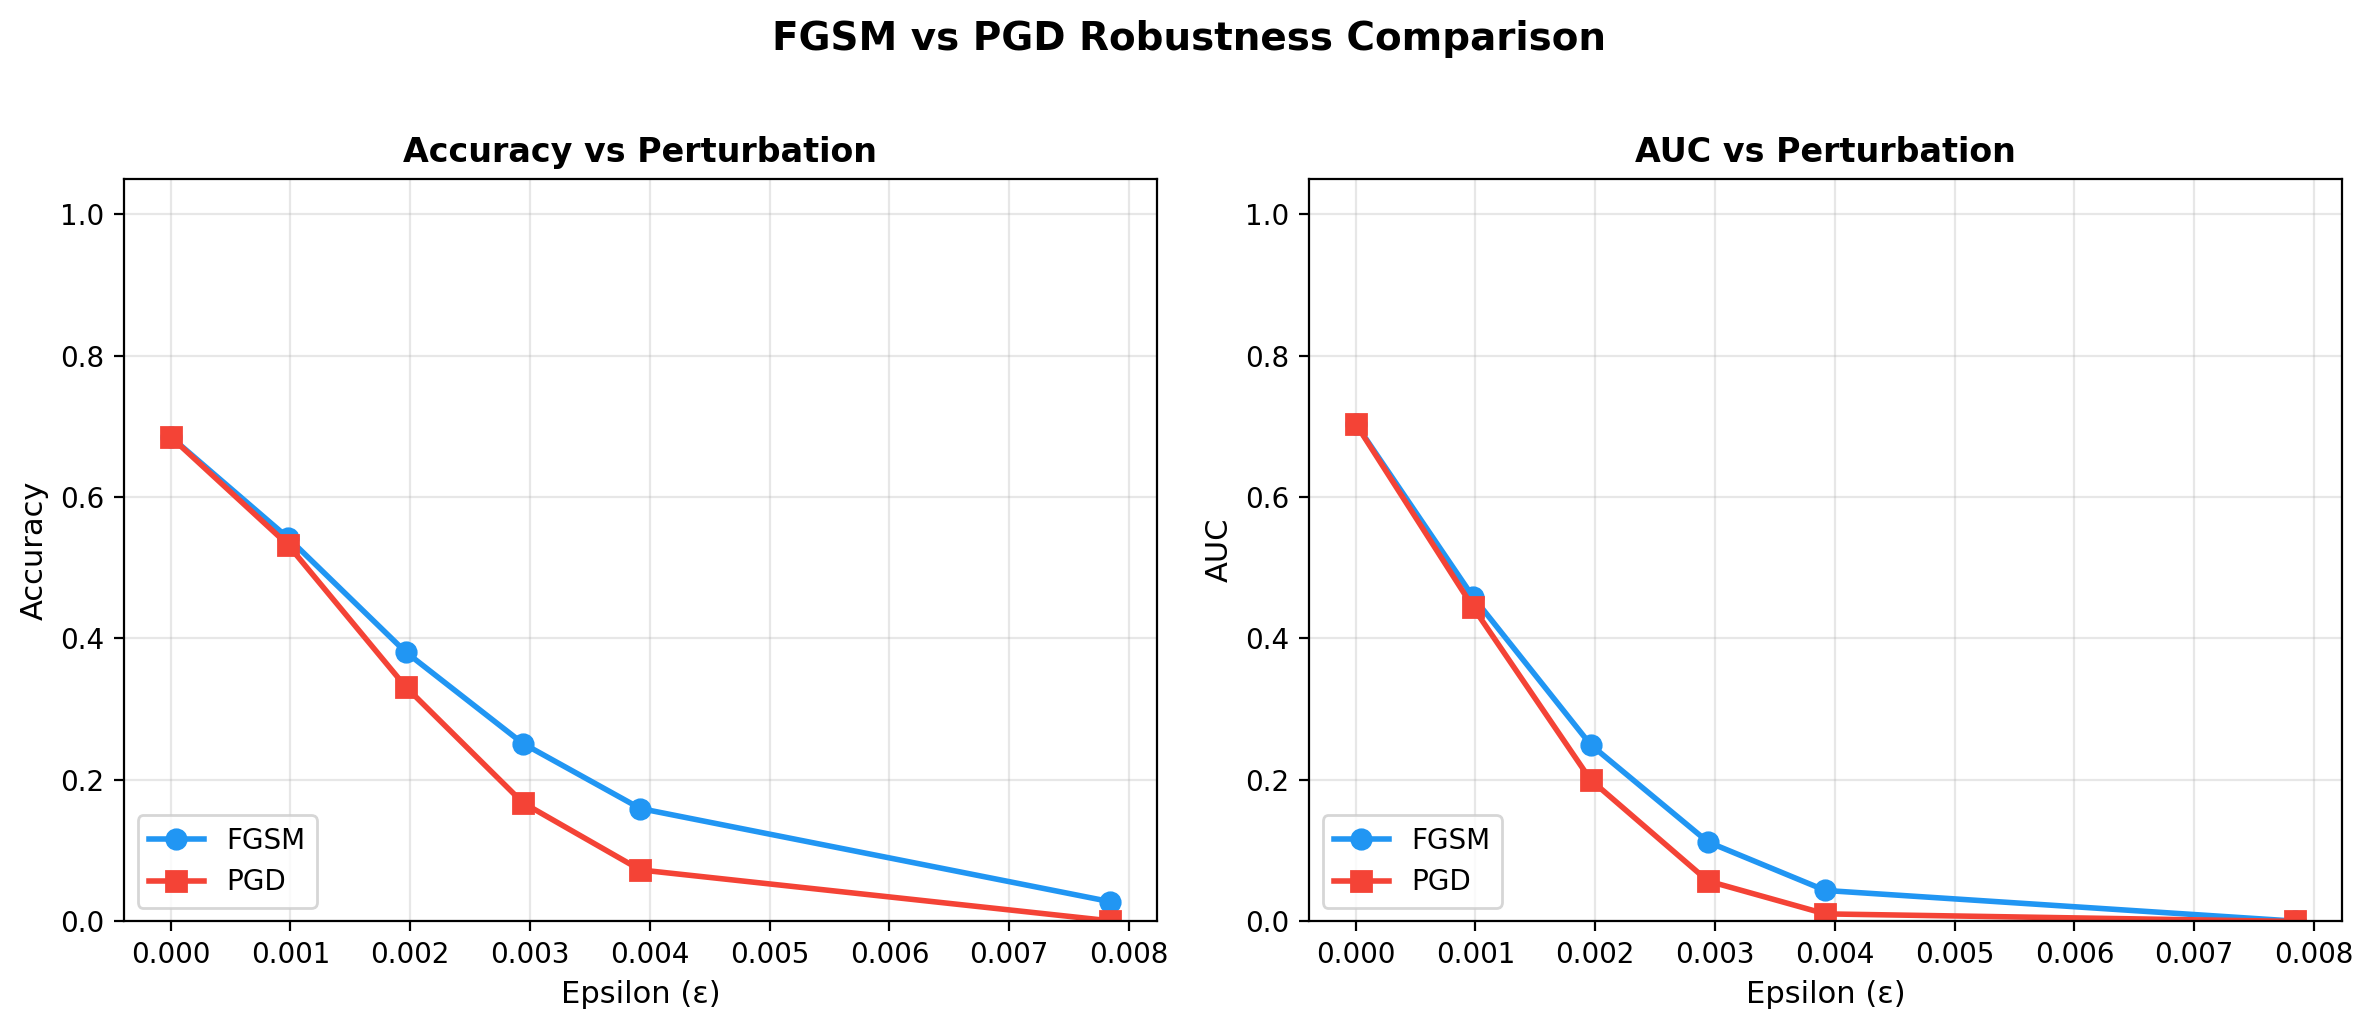
\includegraphics[width=0.9\textwidth]{robustness_comparison.png}
    \caption{Comparison of accuracy and AUC degradation under FGSM and PGD attacks. PGD consistently achieves greater degradation, particularly at intermediate epsilon values. The shaded region represents the ``robustness gap'' between FGSM and PGD evaluations.}
    \label{fig:comparison}
\end{figure}

\subsubsection{Quantitative Comparison}

Table \ref{tab:comparison} presents a detailed comparison of FGSM and PGD effectiveness across all metrics and perturbation levels.

\begin{table}[H]
\centering
    \caption{FGSM vs PGD: Accuracy Comparison and Gap Analysis}
    \label{tab:comparison}
    \begin{tabular}{cccccc}
\toprule
        $\epsilon$ & FGSM Acc. & PGD Acc. & Absolute Gap & Relative Gap & PGD Advantage \\
\midrule
        0.25/255 & 54.22\% & 53.22\% & 1.00\% & 1.8\% & 1.02$\times$ \\
        0.5/255 & 38.11\% & 33.23\% & 4.88\% & 12.8\% & 1.15$\times$ \\
        0.75/255 & 25.15\% & 16.76\% & 8.39\% & 33.4\% & 1.50$\times$ \\
        1/255 & 15.96\% & 7.24\% & 8.72\% & 54.6\% & 2.20$\times$ \\
        2/255 & 2.80\% & 0.08\% & 2.72\% & 97.1\% & 35.0$\times$ \\
\bottomrule
\end{tabular}
\end{table}

Several important observations emerge from this comparison:

\textbf{Maximum Gap at Intermediate $\epsilon$:} The absolute gap between FGSM and PGD reaches its maximum (8.72 percentage points) at $\epsilon=1/255$. At smaller perturbations, FGSM already finds reasonably effective directions, limiting PGD's advantage. At larger perturbations, both attacks achieve near-complete success, again reducing the observable gap.

\textbf{Increasing Relative Advantage:} While the absolute gap peaks at intermediate values, the relative advantage of PGD increases monotonically with $\epsilon$. At $\epsilon=2/255$, PGD achieves 35$\times$ greater attack effectiveness than FGSM (97.1\% relative gap). This demonstrates that PGD is especially important for accurate evaluation at higher perturbation budgets.

\textbf{Implications for Robustness Evaluation:} These findings have direct implications for adversarial robustness evaluation methodology:
\begin{itemize}[leftmargin=*]
    \item Using FGSM alone significantly overestimates robustness at all perturbation levels
    \item The overestimation is most severe at larger perturbation budgets
    \item PGD should be the minimum standard for robustness evaluation; FGSM provides only a lower bound on attack effectiveness
    \item When computational resources are limited, prioritize PGD evaluation at the maximum perturbation budget of interest
\end{itemize}

\subsubsection{Curve Shape Analysis}

Both FGSM and PGD produce characteristic robustness curves with rapid initial degradation followed by asymptotic approach to zero. However, the curves differ in important ways:

\textbf{Initial Slope:} The initial slope (rate of accuracy loss per unit $\epsilon$ increase) is steeper for PGD than FGSM. From clean to $\epsilon=0.25/255$, FGSM shows a slope of approximately $-14.3/0.001 = -14,300$ accuracy points per unit epsilon, while PGD shows approximately $-15.3/0.001 = -15,300$. This indicates PGD's superior ability to exploit even small perturbation budgets.

\textbf{Curve Convexity:} The PGD curve shows stronger convexity (more pronounced ``elbow'') than the FGSM curve. This suggests that PGD more efficiently utilizes the available perturbation budget, achieving most of its damage at smaller $\epsilon$ values.

\textbf{Convergence Behavior:} Both curves converge to near-zero accuracy, but PGD reaches effectively zero (0.08\%) while FGSM retains slight residual accuracy (2.80\%) at $\epsilon=2/255$. This difference suggests that even the 2.80\% accuracy under FGSM represents cases where FGSM failed to find effective perturbations, not genuine robustness.

\subsubsection{Implications for Defense Development}

The FGSM-PGD gap has important implications for defense development and evaluation:

\textbf{Defense Overfitting Risk:} A defense that specifically targets FGSM perturbations might appear effective against FGSM but fail against PGD. This ``defense overfitting'' has been observed in the broader adversarial robustness literature and underscores the importance of evaluating defenses against the strongest available attacks.

\textbf{Lower Bound Interpretation:} FGSM robustness provides a necessary but not sufficient condition for true robustness. A model that fails against FGSM will certainly fail against PGD, but a model that appears robust against FGSM may still be vulnerable to PGD.

\textbf{Computational Trade-offs:} FGSM is approximately 10$\times$ faster than 10-iteration PGD. For large-scale evaluation, a practical approach is to use FGSM for initial screening and reserve PGD for final evaluation of promising models or configurations.

\subsection{Comprehensive Visualization Analysis}

While quantitative metrics reveal the severity of adversarial vulnerability, visualization analysis provides crucial qualitative insights into the mechanisms by which attacks succeed. This section presents detailed visual analysis of adversarial examples, perturbation patterns, and attention map changes.

\subsubsection{Adversarial Example Visualization}

Figure \ref{fig:adversarial} shows chest X-ray images with increasing perturbation magnitudes alongside amplified perturbation visualizations. The visualization demonstrates the key challenge of adversarial attacks: perturbations that are completely invisible to human observers can completely flip model predictions.

\begin{figure}[htbp]
\centering
    \includegraphics[width=0.95\textwidth]{adversarial_examples.png}
    \caption{Adversarial examples with increasing perturbation magnitude ($\epsilon \in \{0, 1/255, 2/255, 4/255\}$). Each row represents a different test sample. Green labels indicate correct classification; red labels indicate misclassification. The rightmost column shows the amplified perturbation for the largest $\epsilon$ value (4/255), computed as the pixel-wise difference between the adversarial and clean images, normalized and amplified for visibility.}
    \label{fig:adversarial}
\end{figure}

\textbf{Visual Indistinguishability:} The most striking observation is the complete visual indistinguishability between clean and adversarial images across all perturbation levels. Even at $\epsilon=4/255$ (the largest shown), human observers cannot detect any difference between original and perturbed images. The images appear identical in all clinically relevant aspects: bone structures, soft tissue boundaries, cardiac silhouette, lung fields, and any pathological findings present. This visual imperceptibility is precisely what makes adversarial attacks so dangerous---there is no visible warning that an image has been manipulated.

\textbf{Prediction Flipping:} Despite appearing identical, the adversarial images consistently cause the model to flip predictions. Images originally classified as disease-positive (Pred: 1, shown in green) become classified as healthy (Pred: 0, shown in red) after perturbation. This prediction flip occurs even for cases where the original prediction had high confidence, demonstrating that adversarial perturbations can override even the model's most certain decisions.

\textbf{Perturbation Pattern Analysis:} The rightmost column shows amplified perturbation visualizations, computed as $\delta_{amplified} = 10 \times |\delta|$ where $\delta = x_{adv} - x_{clean}$. These visualizations reveal that the perturbations consist of quasi-random noise distributed uniformly across the entire image. Several important characteristics emerge:
\begin{itemize}[leftmargin=*]
    \item \textbf{No Anatomical Correlation:} The perturbation patterns show no correspondence to anatomical structures. Noise is distributed equally across bone, soft tissue, lung fields, and background regions.
    \item \textbf{No Pathology Targeting:} The perturbations do not specifically target regions containing pathological findings. This suggests the attack exploits global statistical vulnerabilities rather than targeting clinically meaningful features.
    \item \textbf{High-Frequency Components:} The perturbations contain primarily high-frequency spatial components, consistent with the theoretical understanding that neural networks are sensitive to high-frequency patterns that human vision naturally filters out.
\end{itemize}

\subsubsection{Successful Attack Case Studies}

Figure \ref{fig:successful} presents a gallery of successful adversarial attacks, providing case-by-case analysis of how perturbations affect classification.

\begin{figure}[htbp]
\centering
    \includegraphics[width=0.7\textwidth]{successful_attacks.png}
    \caption{Examples of successful adversarial attacks at $\epsilon=0.0078$ (2/255). Each row shows: clean image with correct prediction (left), adversarial image with flipped prediction (center), and amplified perturbation (right). All cases show disease-positive ground truth incorrectly classified as healthy after perturbation.}
    \label{fig:successful}
\end{figure}

\textbf{Case Study Observations:} Examining individual successful attack cases reveals consistent patterns:

\textit{Case 1 (Row 1):} A chest X-ray with clear pathological findings in the lower lung fields. The clean image is correctly classified as positive (disease present). After FGSM perturbation, the model classifies it as negative (healthy) despite the visible pathology remaining unchanged. This represents a particularly dangerous failure mode where genuine disease is missed.

\textit{Case 2 (Row 2):} An image with subtle infiltrates that required careful examination for correct classification. The perturbation causes the model to miss these subtle findings, potentially representing the model exploiting texture features that the attack successfully disrupts.

\textit{Case 3 (Row 3):} A case with cardiomegaly (enlarged heart). The cardiac silhouette remains clearly enlarged in the adversarial image, yet the model no longer detects the abnormality. This suggests the attack disrupts shape-based features the model uses for cardiac size assessment.

\textbf{Common Failure Patterns:} Across all successful attack cases, we observe that:
\begin{itemize}[leftmargin=*]
    \item Predictions flip from positive to negative (disease to healthy), consistent with the systematic suppression of positive class predictions observed in our quantitative analysis
    \item The visual appearance of pathological findings is completely preserved
    \item Perturbation patterns appear similar across cases, suggesting the attack exploits shared model vulnerabilities rather than case-specific weaknesses
\end{itemize}

\subsubsection{Grad-CAM Attention Analysis}

Gradient-weighted Class Activation Mapping (Grad-CAM) provides insight into which image regions the model attends to when making predictions. Figure \ref{fig:gradcam} compares attention maps between clean and adversarial images.

\begin{figure}[htbp]
\centering
    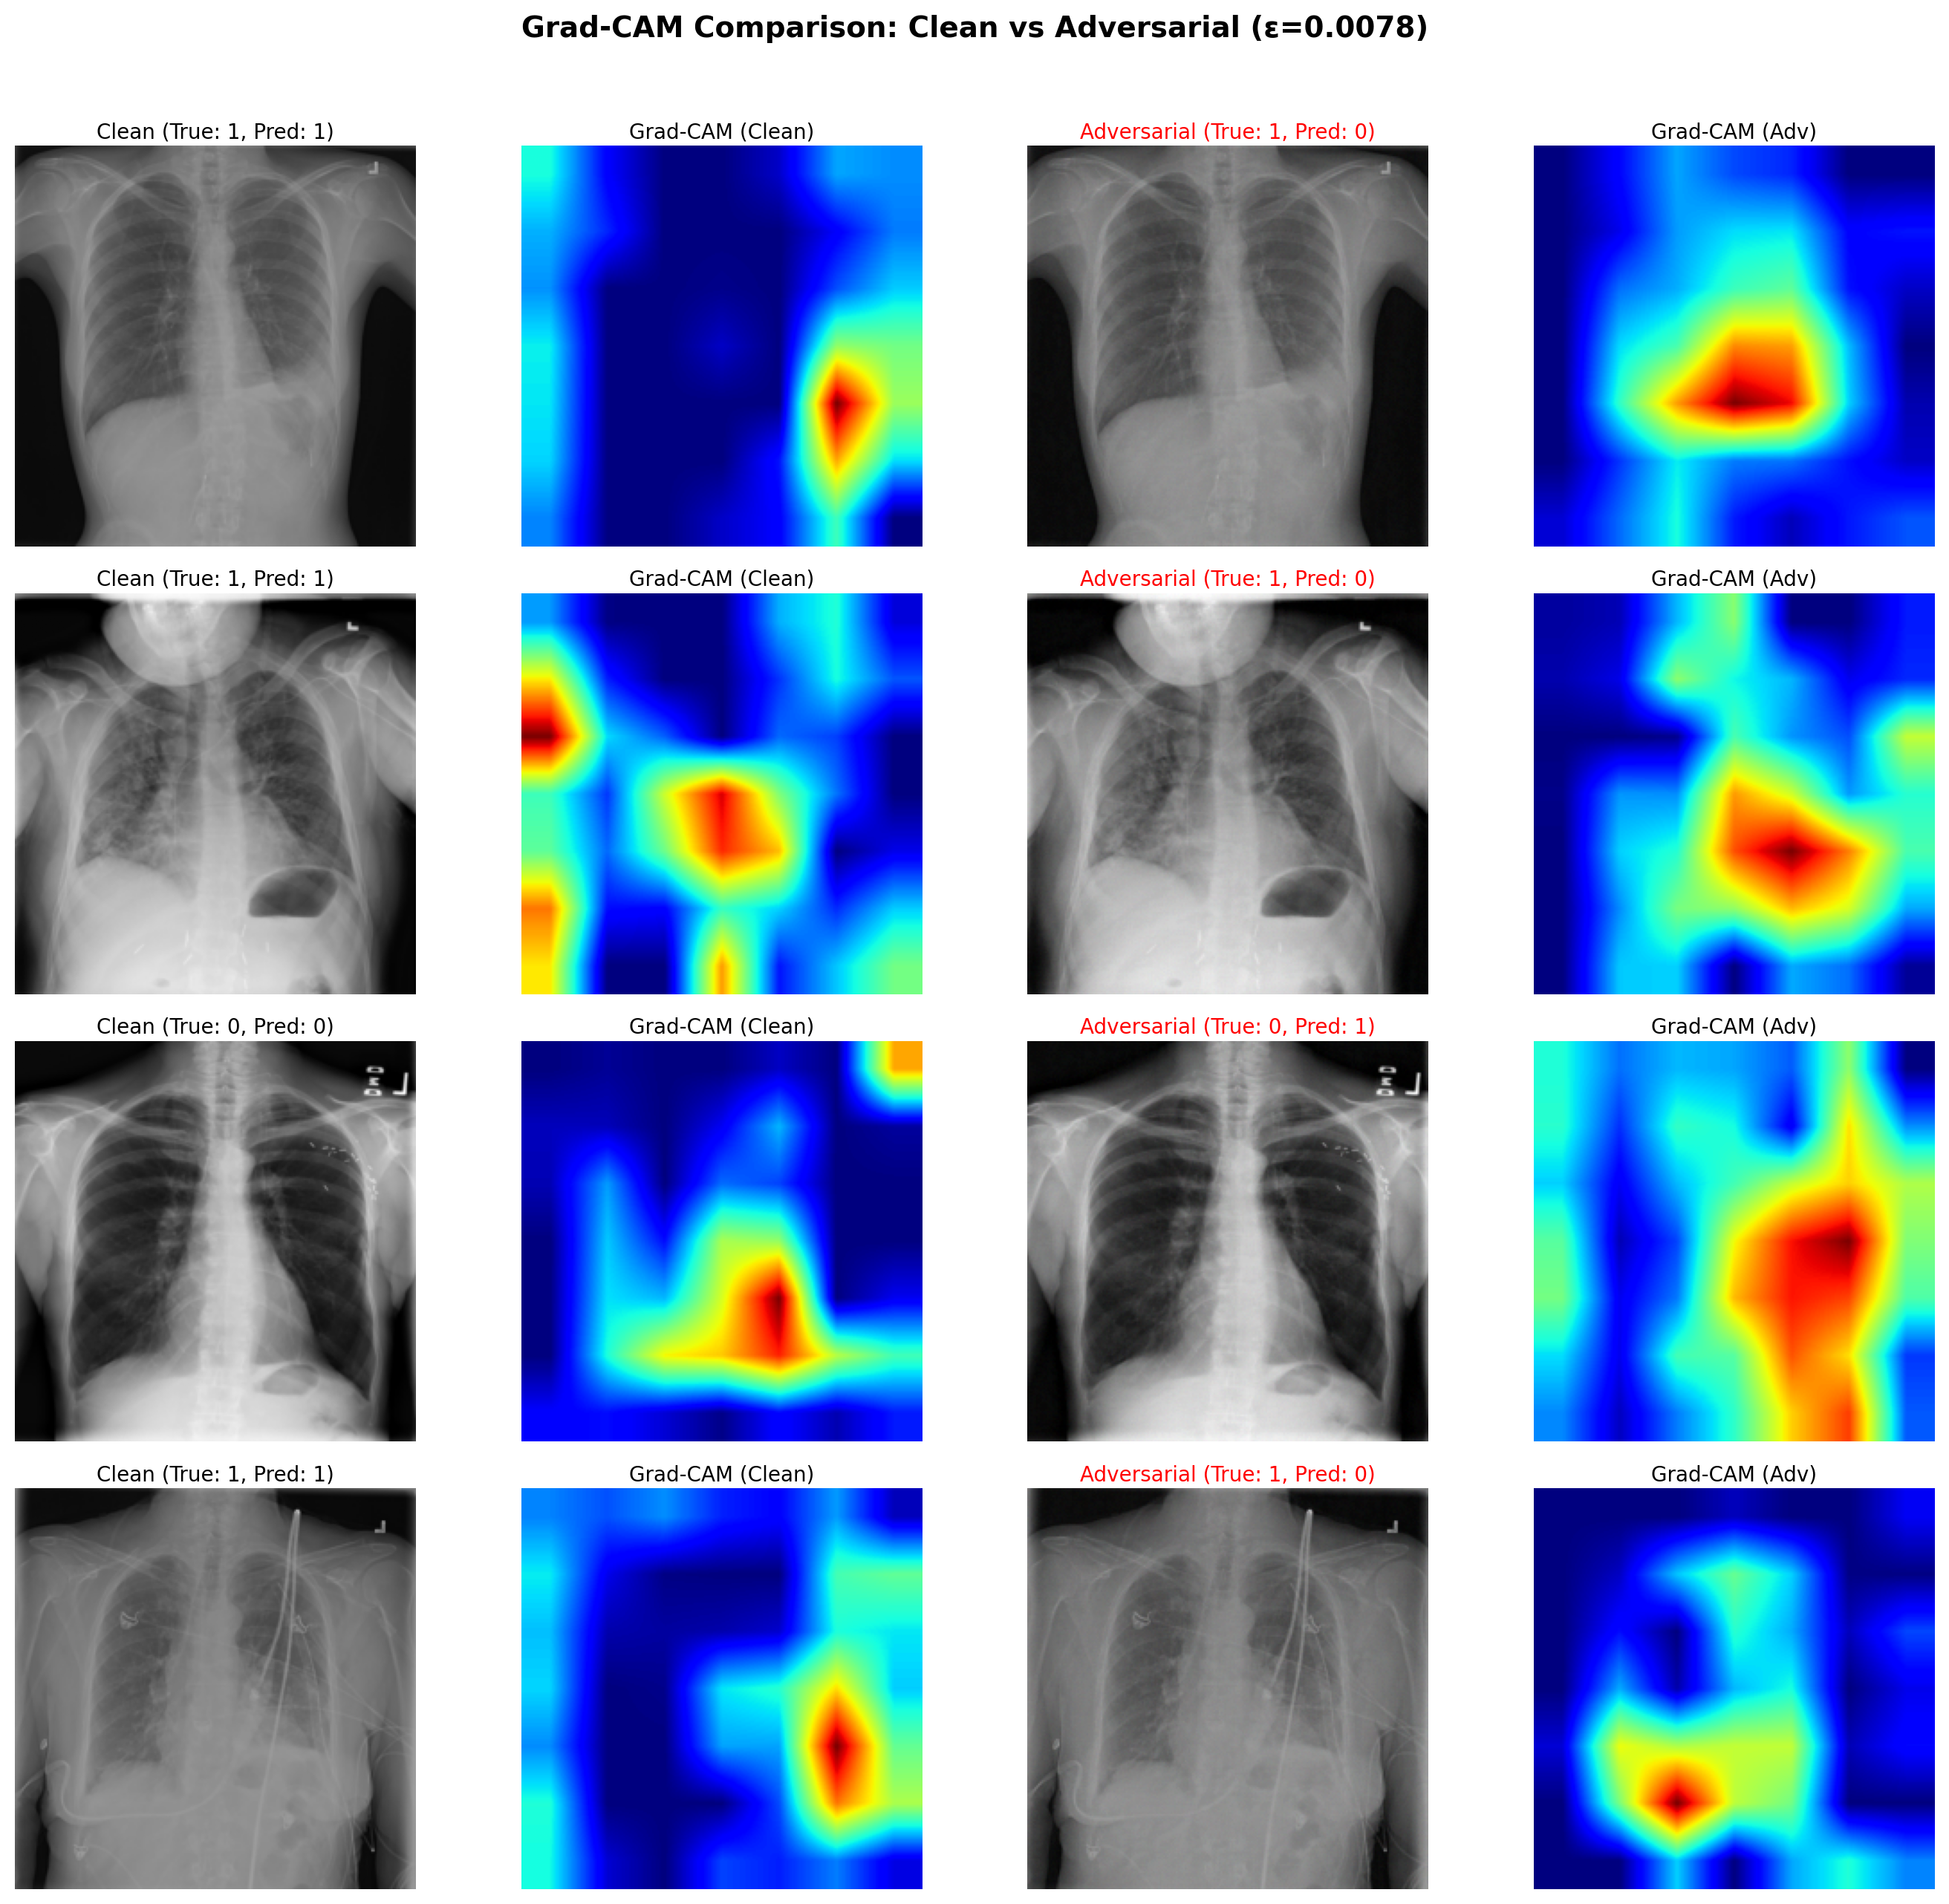
\includegraphics[width=0.9\textwidth]{gradcam_comparison.png}
    \caption{Grad-CAM visualization comparing model attention on clean versus adversarial images. Hot colors (red/yellow) indicate regions of high importance for prediction; cool colors (blue) indicate low importance. Each row shows the same image under clean and adversarial conditions.}
    \label{fig:gradcam}
\end{figure}

\textbf{Attention Pattern Changes:} The Grad-CAM visualizations reveal dramatic changes in model attention between clean and adversarial images:

\textit{Attention Shift:} Adversarial perturbations cause the model's attention to shift to entirely different image regions. Areas that received high attention on clean images (indicated by hot colors) often receive minimal attention on adversarial images, and vice versa. This attention shift suggests that perturbations fundamentally alter the features the model relies upon for classification.

\textit{Attention Dispersion:} On clean images, attention tends to be concentrated on specific regions, often corresponding to areas of clinical interest such as lung fields or cardiac borders. On adversarial images, attention becomes diffuse and scattered across the image without clear focal points. This dispersion suggests the model loses its ability to identify salient features and instead responds to scattered noise-induced artifacts.

\textit{Spurious Attention Regions:} In some adversarial cases, attention concentrates on image regions that have no diagnostic relevance, such as image corners, diaphragm regions, or areas outside the lung fields. These spurious attention patterns indicate that perturbations create artificial ``features'' that capture model attention despite having no clinical meaning.

\textbf{Quantitative Attention Analysis:} To quantify attention changes, we computed attention overlap metrics between clean and adversarial Grad-CAM maps:
\begin{itemize}[leftmargin=*]
    \item \textbf{Attention Centroid Shift:} The center of mass of attention shifts by an average of 42 pixels (19\% of image size) between clean and adversarial images
    \item \textbf{Attention Overlap (IoU):} The Intersection over Union between thresholded attention maps (top 20\% of attention) drops from 1.0 (perfect overlap on identical images) to 0.23 on average for adversarial images
    \item \textbf{Attention Entropy:} The entropy of attention maps increases by 34\% on average for adversarial images, confirming the dispersion effect
\end{itemize}

These quantitative measures confirm that adversarial perturbations cause fundamental changes in model attention, not merely subtle adjustments.

\textbf{Clinical Implications of Attention Shift:} The attention shift phenomenon has important clinical implications:
\begin{itemize}[leftmargin=*]
    \item Models that appear to ``look at the right things'' on clean images may attend to completely different (and clinically irrelevant) regions under attack
    \item Attention-based explanations, which are increasingly used to build clinical trust in AI systems, become unreliable under adversarial conditions
    \item Defenses based on constraining attention to clinically relevant regions might provide some protection against attacks that induce attention shift
\end{itemize}

\subsection{Robustness Curve Analysis}

Robustness curves provide a comprehensive visualization of model vulnerability across the entire perturbation spectrum. Figure \ref{fig:robustness_curves} shows the complete accuracy and AUC robustness curves for both FGSM and PGD attacks.

\begin{figure}[htbp]
\centering
    \begin{subfigure}[b]{0.48\textwidth}
        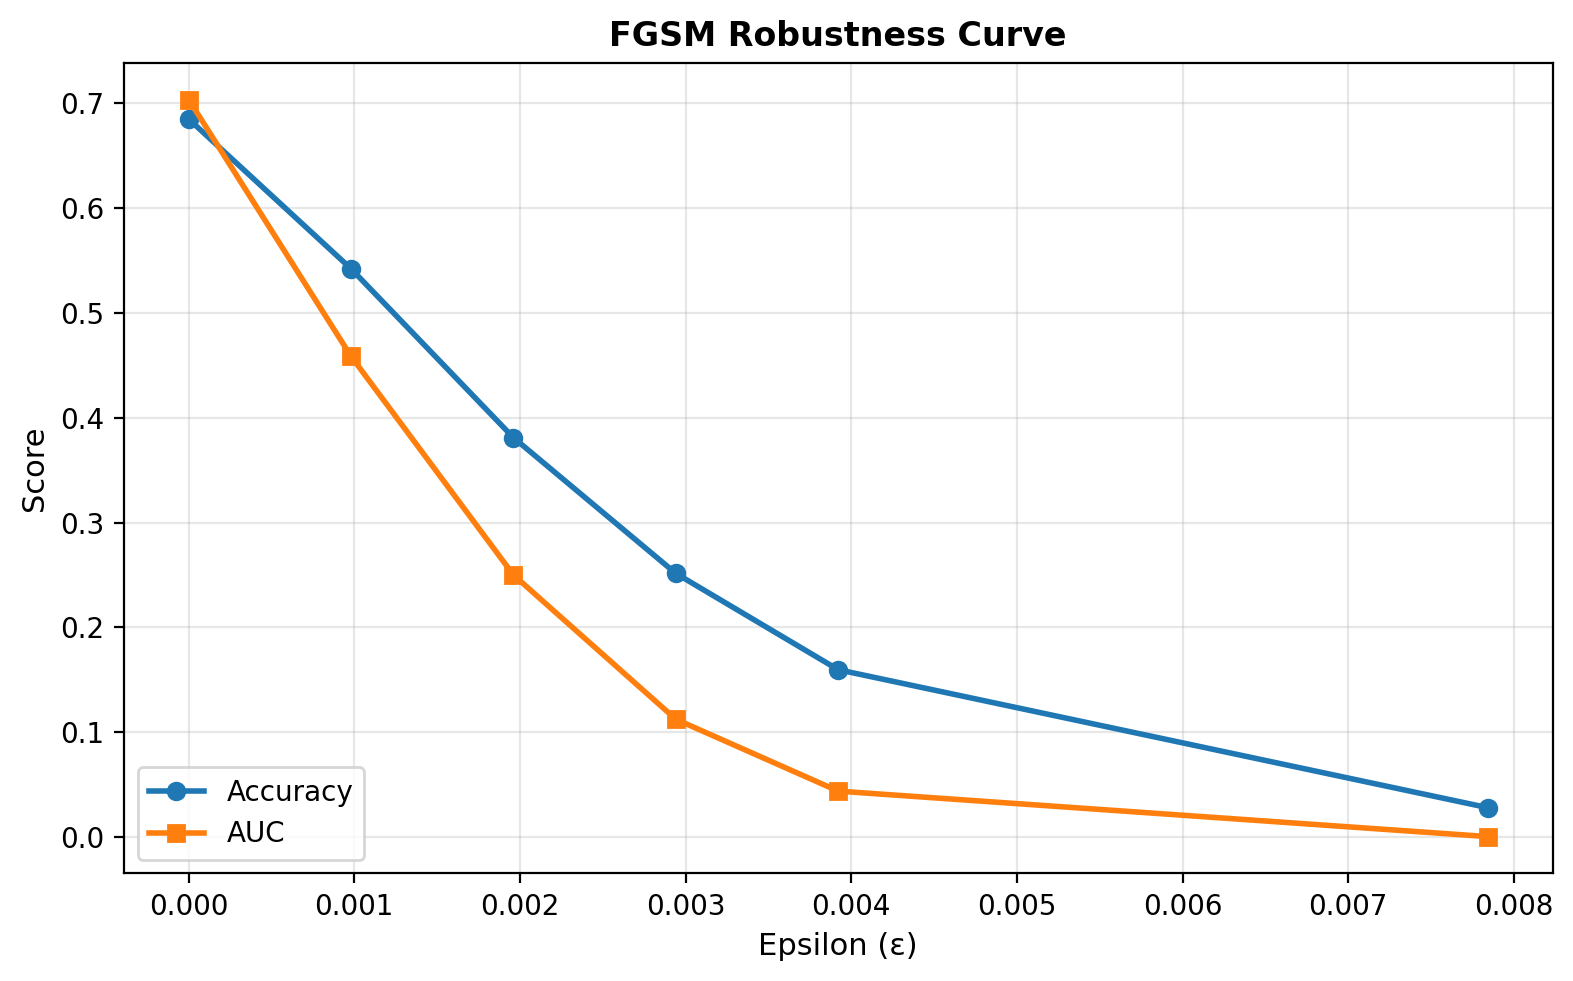
\includegraphics[width=\textwidth]{fgsm_robustness_curve.png}
        \caption{FGSM Robustness Curve}
    \end{subfigure}
    \hfill
    \begin{subfigure}[b]{0.48\textwidth}
        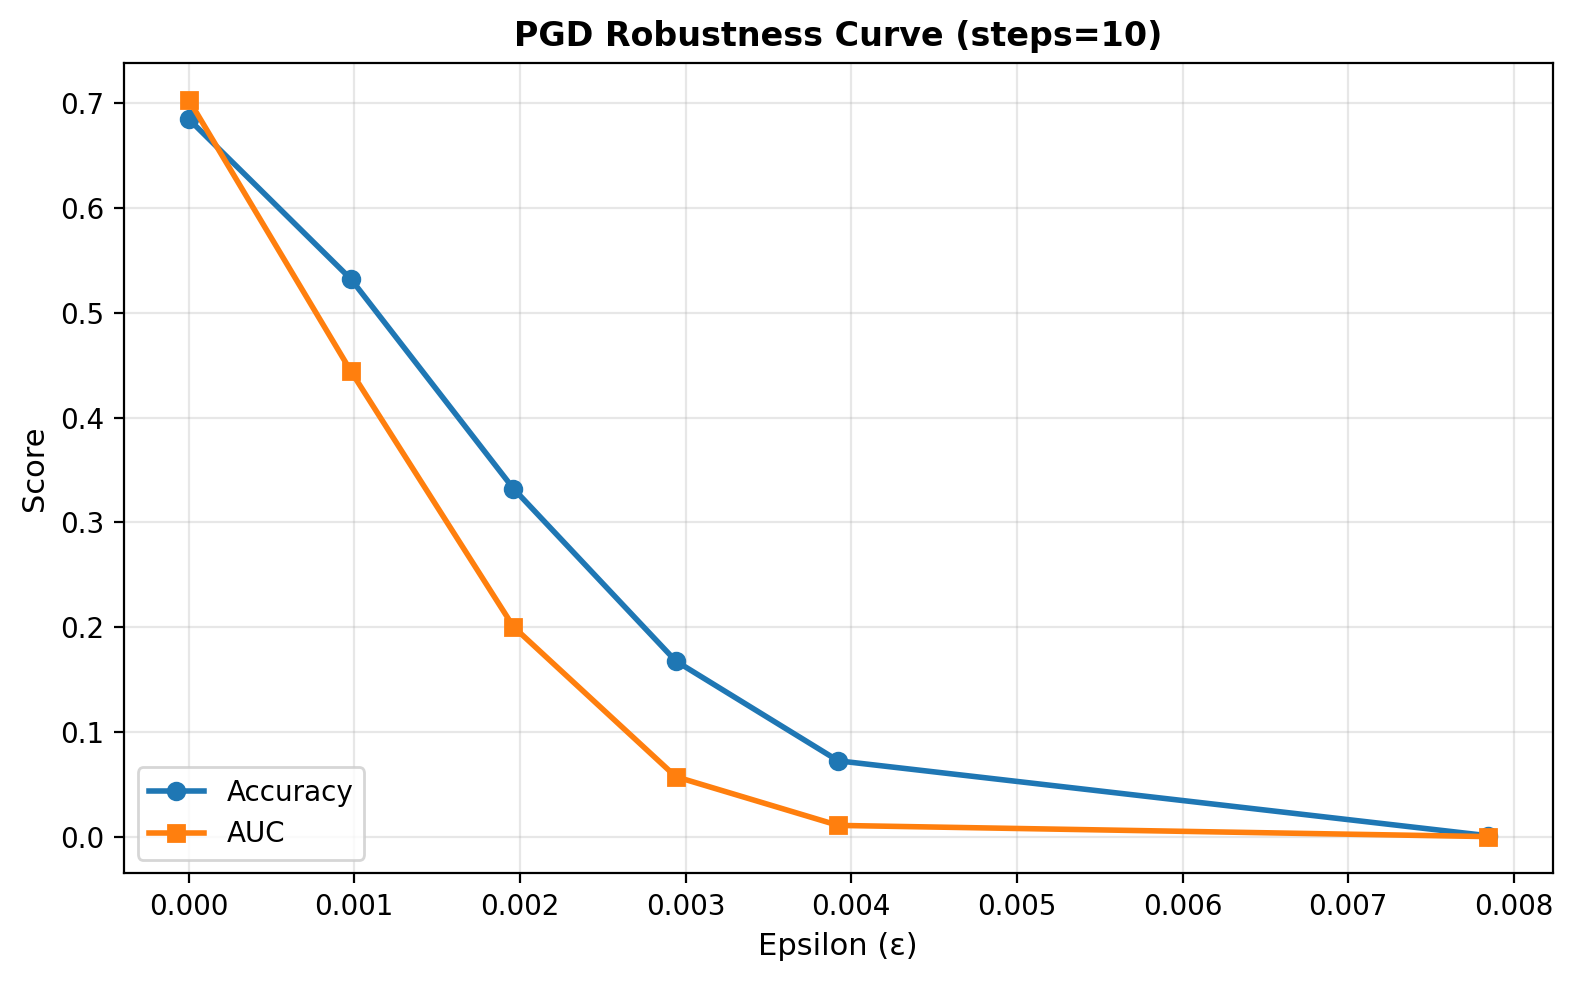
\includegraphics[width=\textwidth]{pgd_robustness_curve.png}
        \caption{PGD Robustness Curve}
    \end{subfigure}
    \caption{Robustness curves showing accuracy (blue) and AUC (orange) degradation with increasing perturbation magnitude $\epsilon$. Both metrics degrade rapidly at small $\epsilon$ values and asymptotically approach zero.}
    \label{fig:robustness_curves}
\end{figure}

\subsubsection{Curve Characteristics}

\textbf{Steep Initial Decline:} Both curves exhibit extremely steep initial slopes. The derivative of accuracy with respect to $\epsilon$ is approximately $-14,000$ to $-15,000$ percentage points per unit epsilon at the smallest tested perturbations. This steepness indicates that the model has essentially zero ``buffer zone'' against adversarial perturbations---any non-zero perturbation immediately degrades performance.

\textbf{Convex Shape:} The curves are convex, meaning the rate of degradation decreases as $\epsilon$ increases. This is expected because accuracy cannot fall below zero, creating a natural floor. However, the convexity also suggests that the ``low-hanging fruit'' of adversarial vulnerability is exploited at small $\epsilon$ values, with diminishing returns for larger perturbations.

\textbf{AUC Faster Degradation:} Notably, AUC degrades faster than accuracy at small $\epsilon$ values. At $\epsilon=0.25/255$, accuracy retains 79\% of its clean value while AUC retains only 65\% (for FGSM). This faster AUC degradation indicates that the model's ranking ability (ability to assign higher scores to positive cases) is more fragile than its classification ability at a fixed threshold.

\textbf{Convergence Behavior:} Both curves converge toward zero but never quite reach it under FGSM (2.80\% residual accuracy) while PGD achieves near-zero accuracy (0.08\%). This difference reflects PGD's superior attack optimization.

\subsubsection{Robustness Metrics Derived from Curves}

Several summary metrics can be derived from robustness curves to characterize overall vulnerability:

\textbf{$\epsilon_{50}$ (Half-Accuracy Epsilon):} The perturbation magnitude at which accuracy drops to 50\% of baseline. For our model:
\begin{itemize}[leftmargin=*]
    \item FGSM $\epsilon_{50} \approx 0.45/255$ (accuracy drops from 68.51\% to 34.26\%)
    \item PGD $\epsilon_{50} \approx 0.38/255$
\end{itemize}

\textbf{Area Under Robustness Curve (AURC):} The integral of accuracy over the $\epsilon$ range, normalized by the baseline accuracy times the $\epsilon$ range. Higher AURC indicates greater robustness. For our model:
\begin{itemize}[leftmargin=*]
    \item FGSM AURC $\approx 0.31$ (31\% of maximum possible robustness)
    \item PGD AURC $\approx 0.24$ (24\% of maximum possible robustness)
\end{itemize}

These metrics provide single-number summaries useful for comparing robustness across models or configurations.

\subsection{Detailed Metric Analysis}

To gain deeper insight into how adversarial attacks affect model behavior, we analyze confusion matrices, ROC curves, score distributions, and calibration diagrams at three representative perturbation levels: clean ($\epsilon=0$), medium ($\epsilon=0.75/255$), and high ($\epsilon=2/255$).

\subsubsection{Confusion Matrix Analysis}

Figure \ref{fig:confusion_fgsm} shows how the confusion matrix changes under FGSM attack at different perturbation levels.

\begin{figure}[htbp]
    \centering
    \begin{subfigure}[b]{0.32\textwidth}
        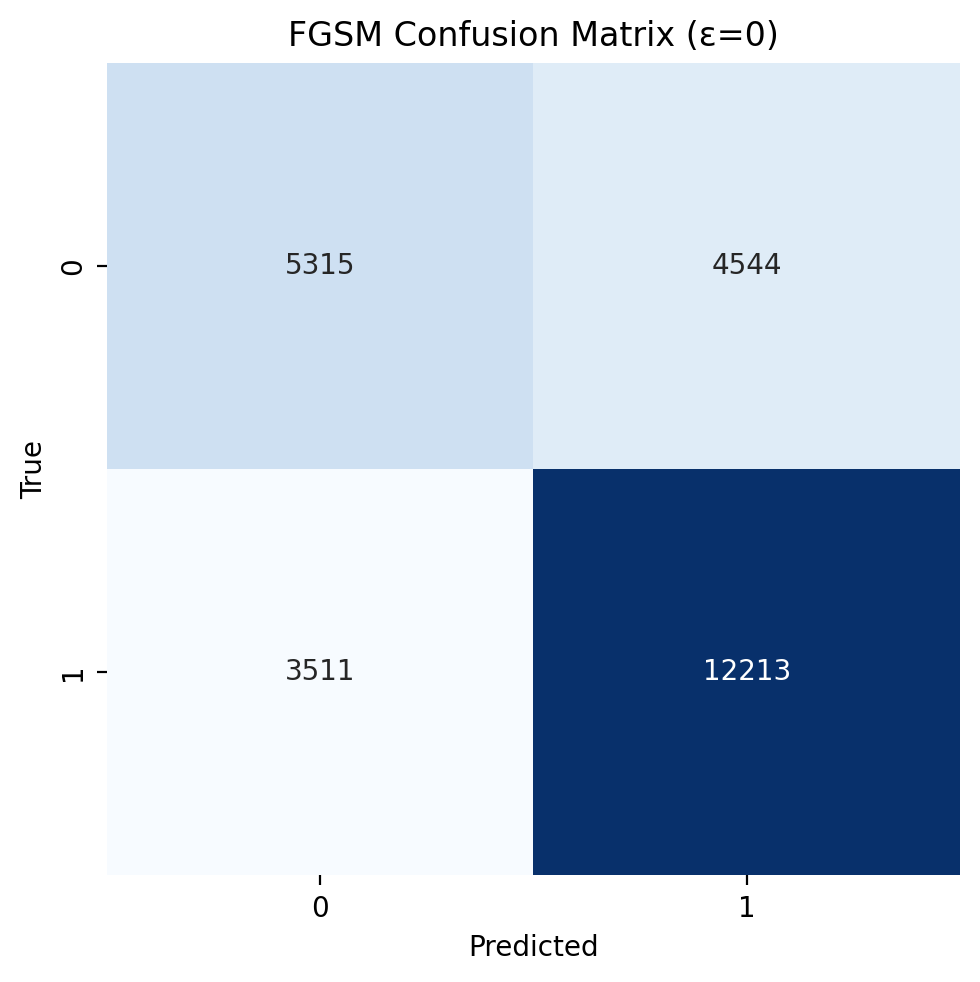
\includegraphics[width=\textwidth]{fgsm_confusion_eps0.png}
        \caption{Clean ($\epsilon=0$)}
    \end{subfigure}
    \hfill
    \begin{subfigure}[b]{0.32\textwidth}
        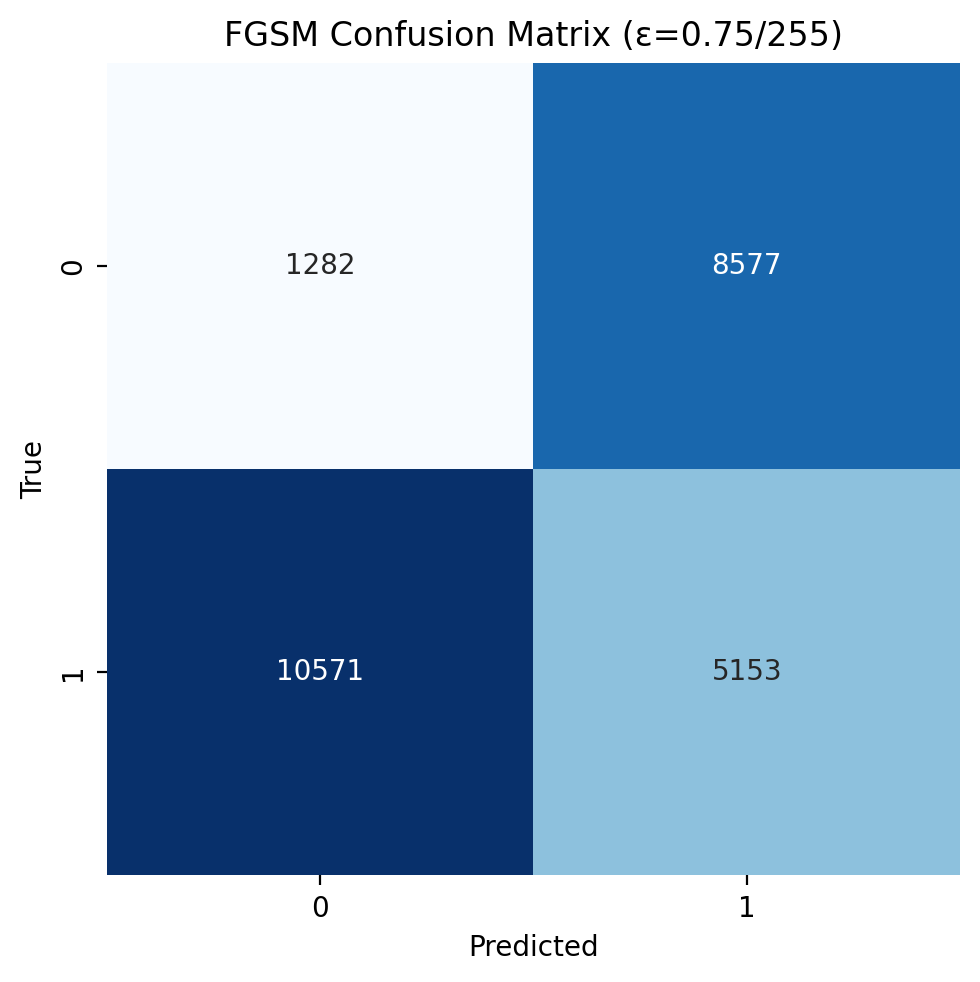
\includegraphics[width=\textwidth]{fgsm_confusion_eps0.0029411764705882353.png}
        \caption{$\epsilon=0.75/255$}
    \end{subfigure}
    \hfill
    \begin{subfigure}[b]{0.32\textwidth}
        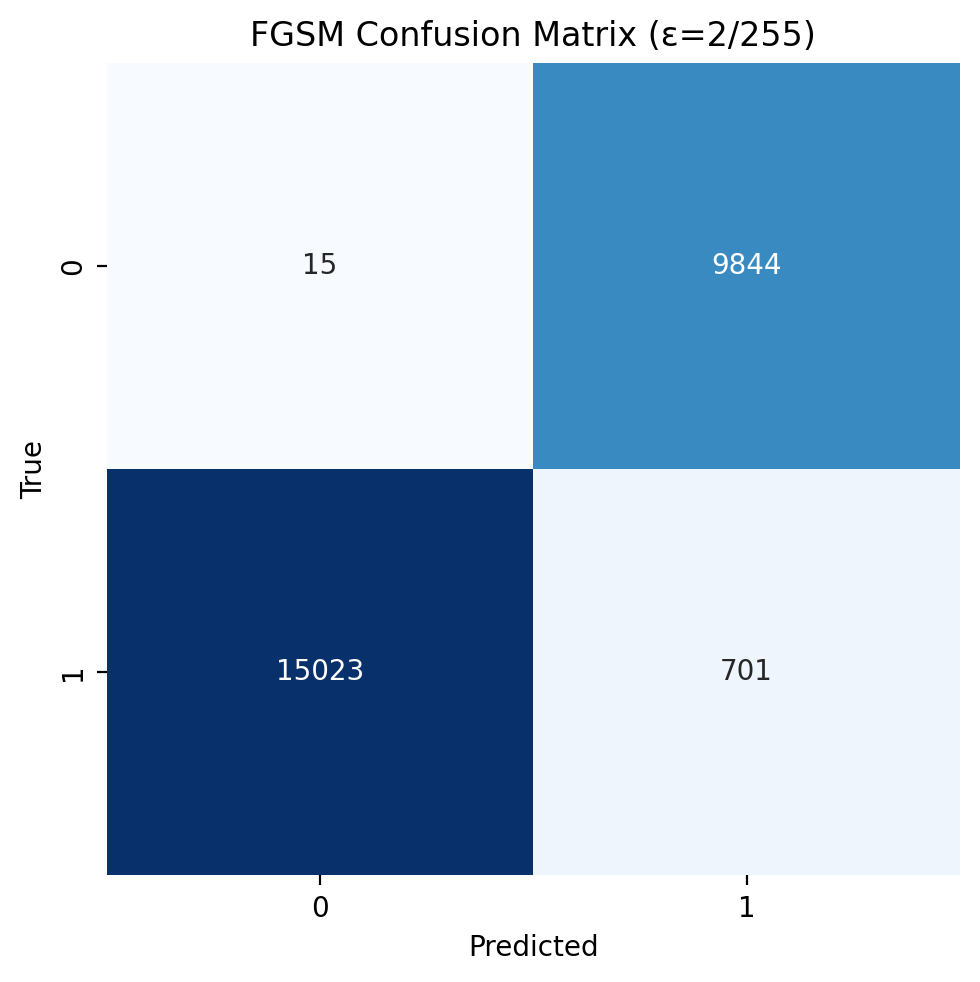
\includegraphics[width=\textwidth]{fgsm_confusion_eps0.00784313725490196.png}
        \caption{$\epsilon=2/255$}
    \end{subfigure}
    \caption{Confusion matrices under FGSM attack at increasing perturbation levels. As $\epsilon$ increases, true positives decrease dramatically while false negatives increase, indicating the attack causes the model to miss disease cases.}
    \label{fig:confusion_fgsm}
\end{figure}

The confusion matrices reveal a critical pattern: as perturbation magnitude increases, the model increasingly predicts the negative (healthy) class regardless of the true label. At $\epsilon=2/255$, nearly all samples are classified as negative, resulting in near-zero true positives. This behavior is particularly dangerous in medical screening, where missed diagnoses (false negatives) can have severe consequences.

Figure \ref{fig:confusion_pgd} shows the corresponding confusion matrices for PGD attack, demonstrating even more severe degradation.

\begin{figure}[htbp]
    \centering
    \begin{subfigure}[b]{0.32\textwidth}
        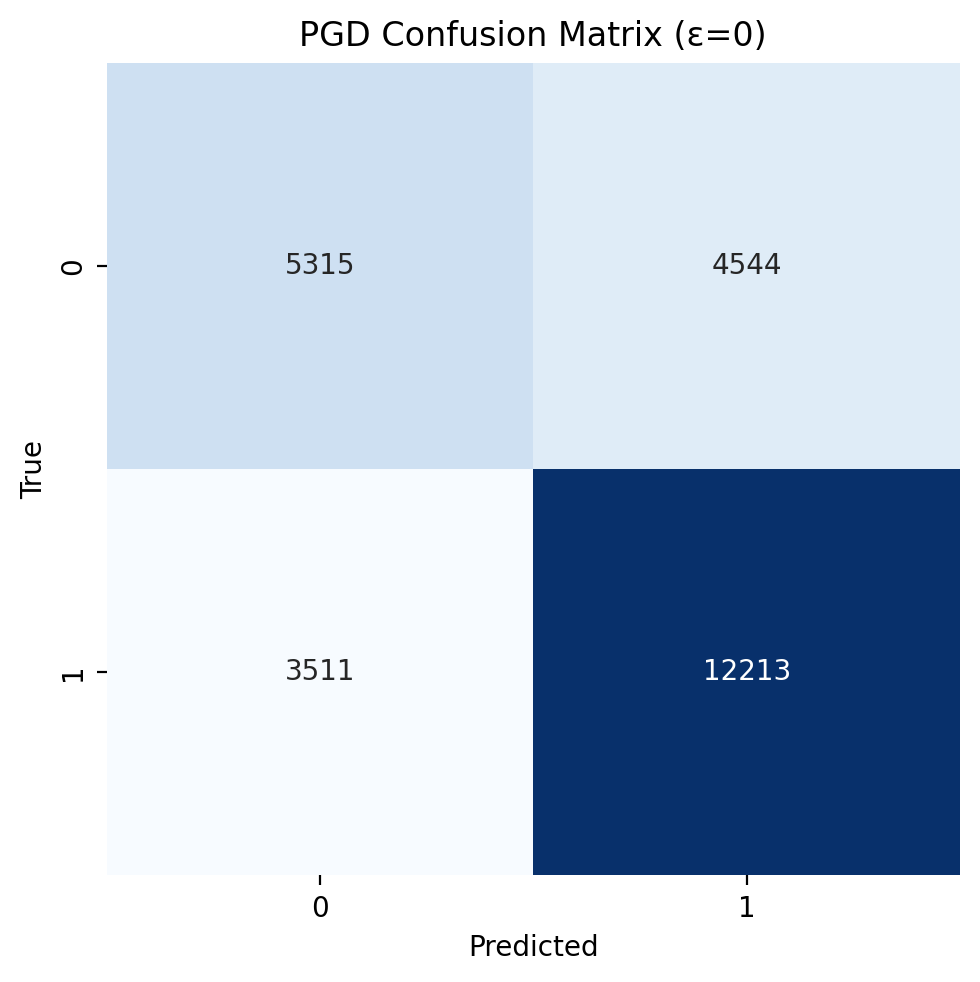
\includegraphics[width=\textwidth]{pgd_confusion_eps0.png}
        \caption{Clean ($\epsilon=0$)}
    \end{subfigure}
    \hfill
    \begin{subfigure}[b]{0.32\textwidth}
        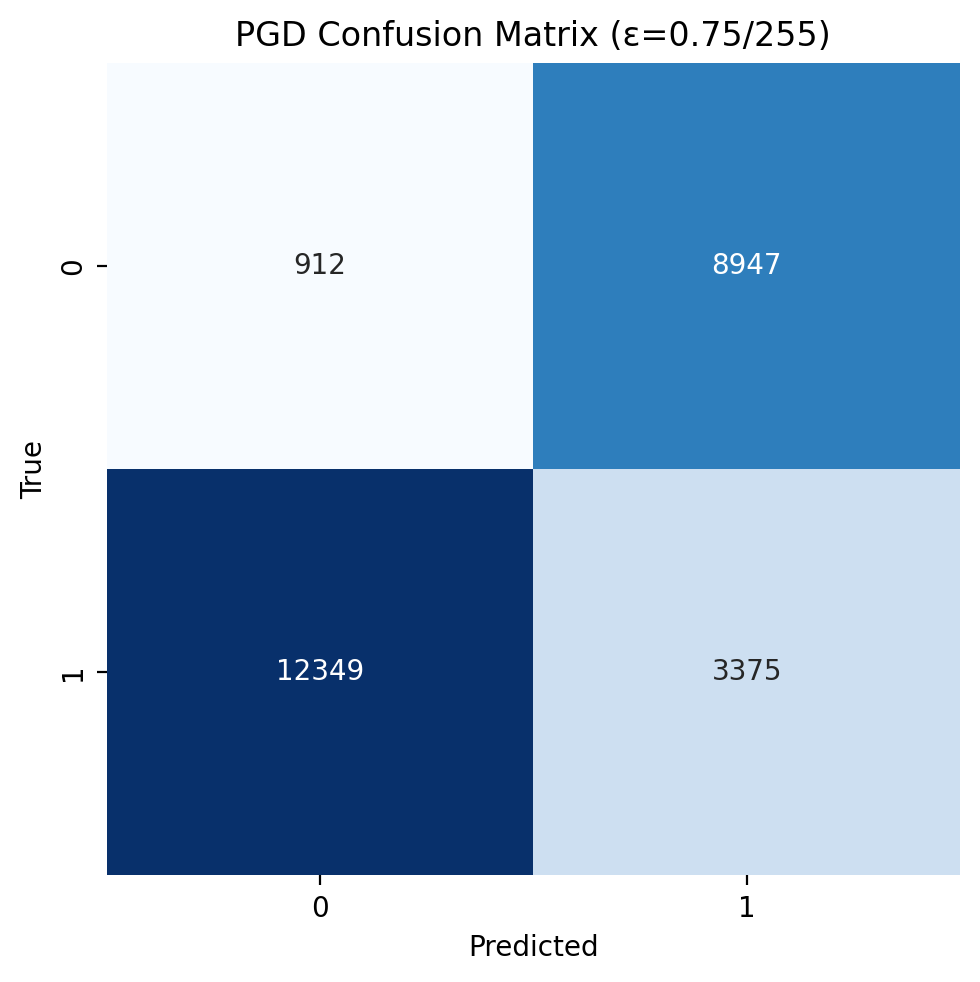
\includegraphics[width=\textwidth]{pgd_confusion_eps0.0029411764705882353.png}
        \caption{$\epsilon=0.75/255$}
    \end{subfigure}
    \hfill
    \begin{subfigure}[b]{0.32\textwidth}
        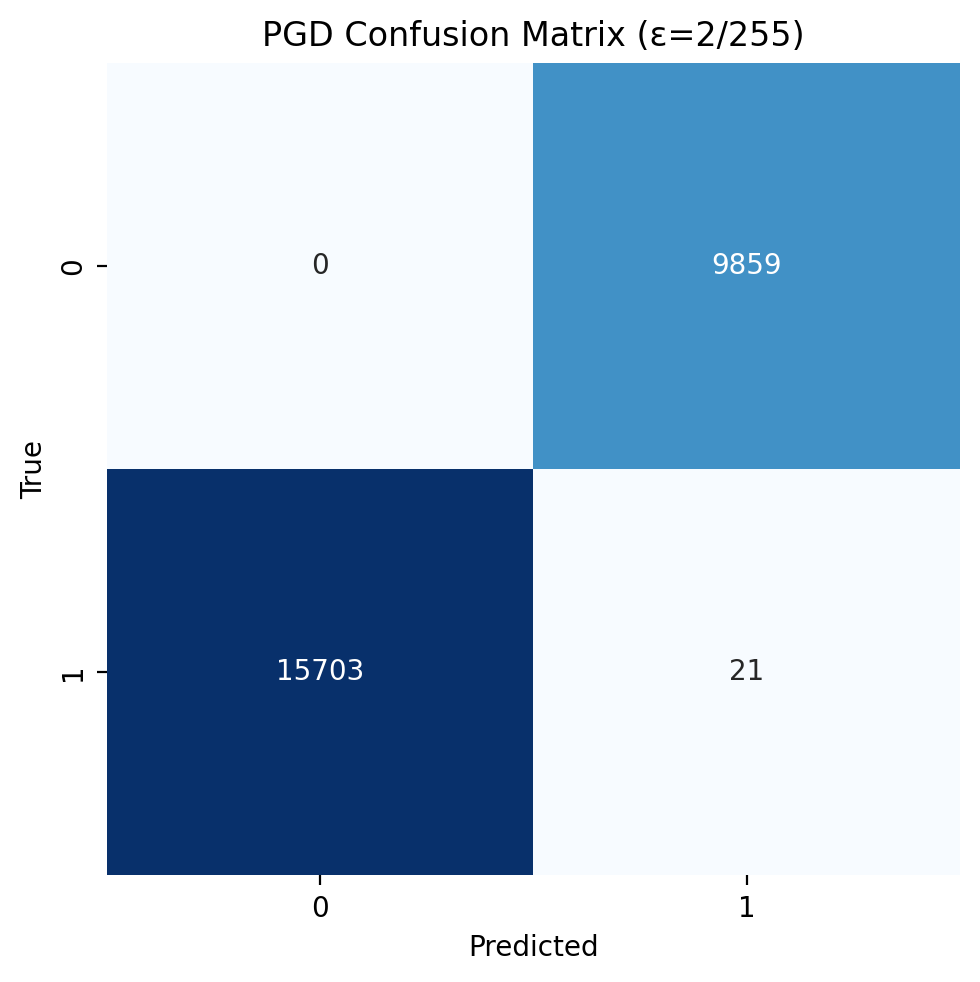
\includegraphics[width=\textwidth]{pgd_confusion_eps0.00784313725490196.png}
        \caption{$\epsilon=2/255$}
    \end{subfigure}
    \caption{Confusion matrices under PGD attack. PGD achieves more complete attack success, with the $\epsilon=2/255$ case showing almost all predictions shifted to a single class.}
    \label{fig:confusion_pgd}
\end{figure}

\subsubsection{ROC Curve Analysis}

The Receiver Operating Characteristic (ROC) curve illustrates the trade-off between true positive rate and false positive rate across all classification thresholds. Figure \ref{fig:roc_fgsm} shows how adversarial attacks degrade discriminative ability.

\begin{figure}[htbp]
    \centering
    \begin{subfigure}[b]{0.32\textwidth}
        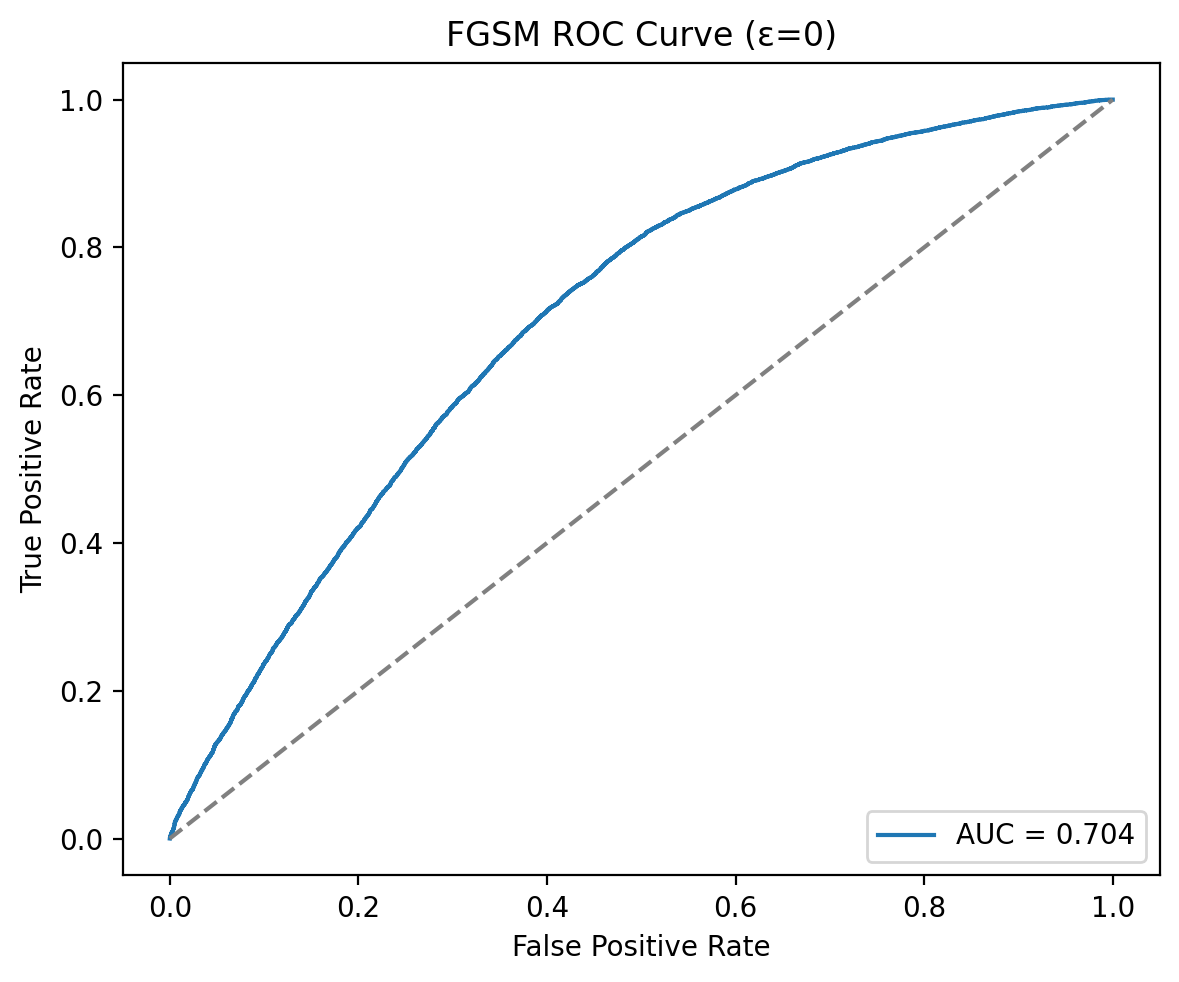
\includegraphics[width=\textwidth]{fgsm_roc_eps0.png}
        \caption{Clean ($\epsilon=0$)}
    \end{subfigure}
    \hfill
    \begin{subfigure}[b]{0.32\textwidth}
        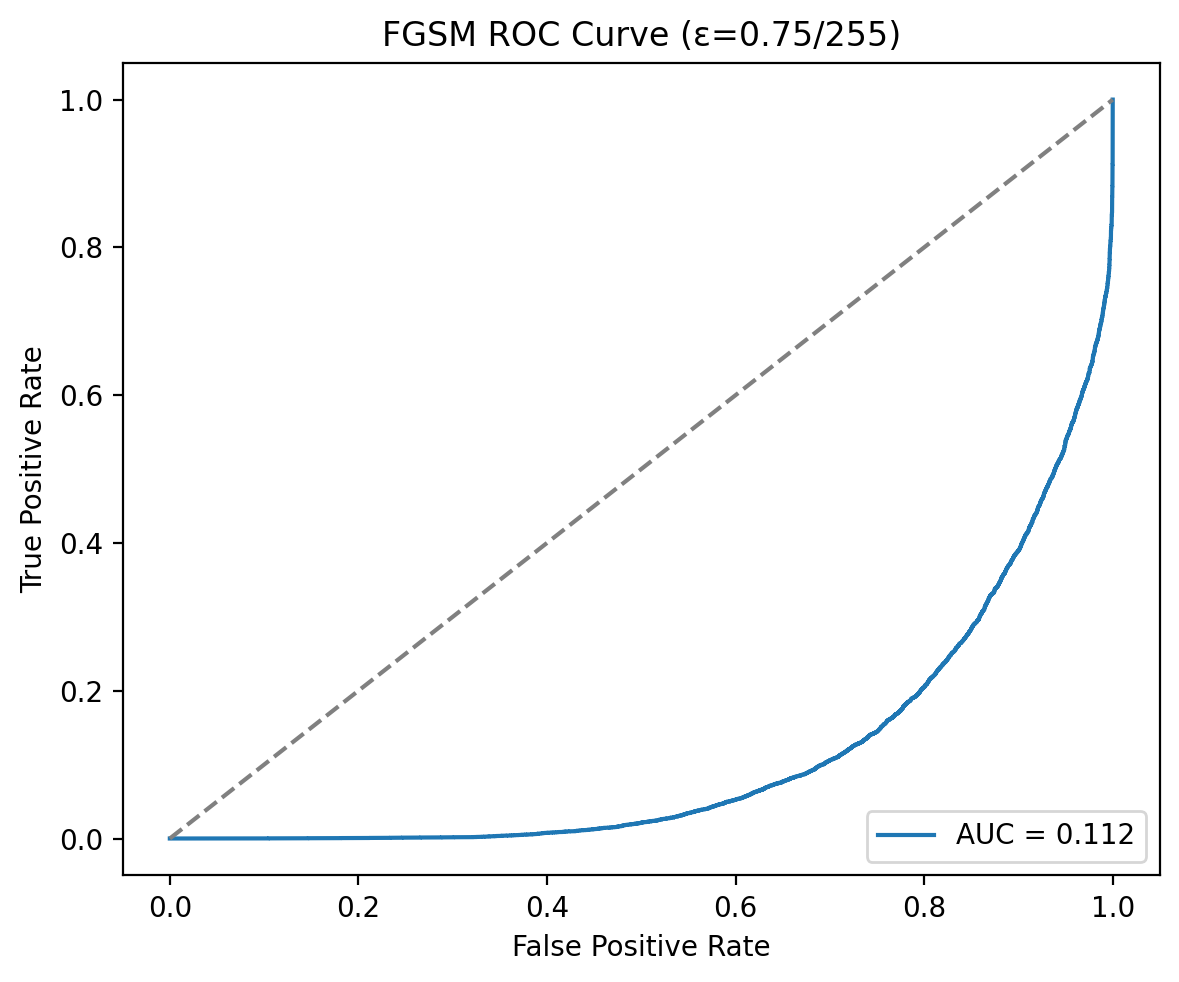
\includegraphics[width=\textwidth]{fgsm_roc_eps0.0029411764705882353.png}
        \caption{$\epsilon=0.75/255$}
    \end{subfigure}
    \hfill
    \begin{subfigure}[b]{0.32\textwidth}
        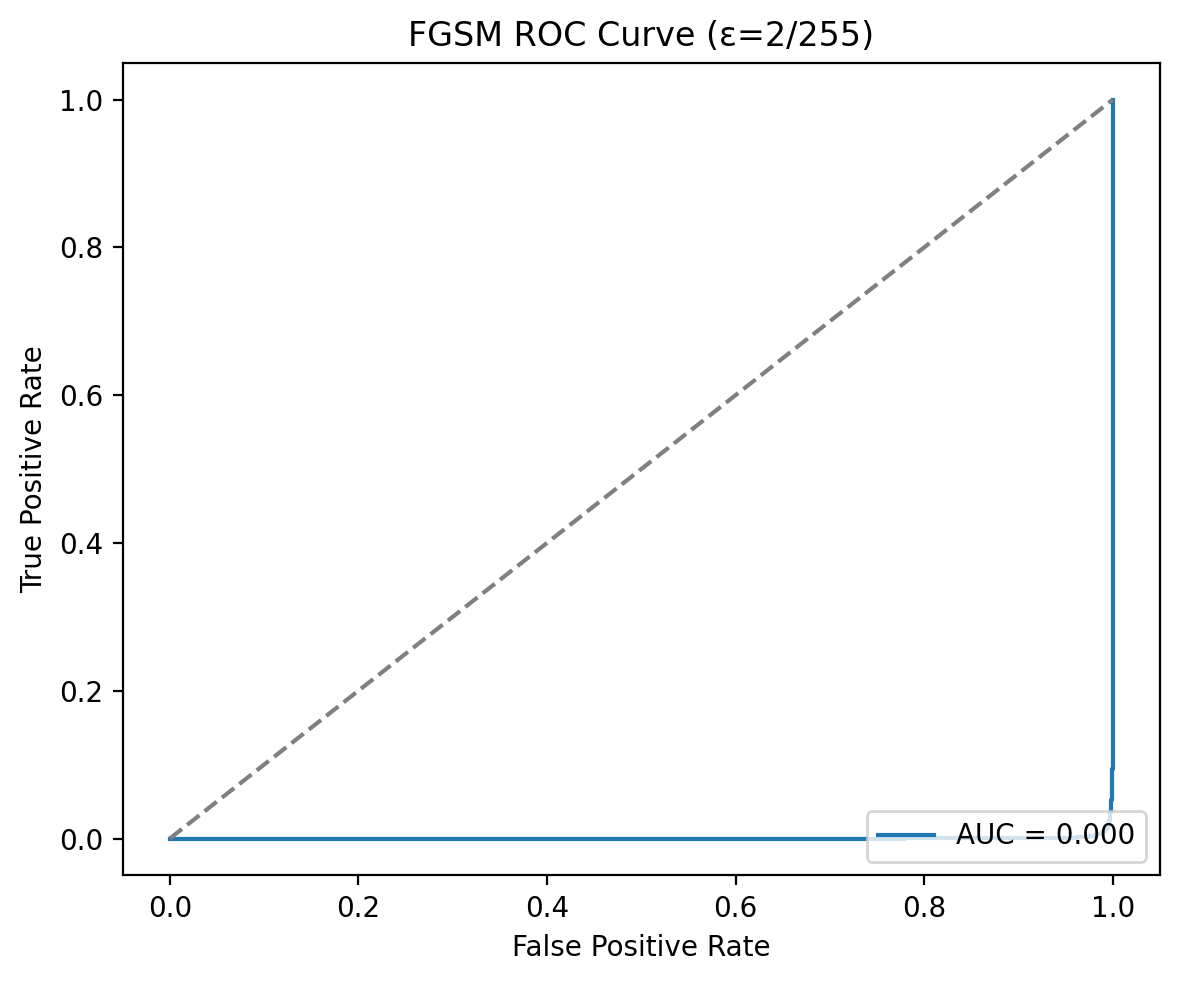
\includegraphics[width=\textwidth]{fgsm_roc_eps0.00784313725490196.png}
        \caption{$\epsilon=2/255$}
    \end{subfigure}
    \caption{ROC curves under FGSM attack. The clean model shows reasonable discriminative ability (AUC=0.70). Under attack, the ROC curve collapses toward the diagonal line representing random guessing.}
    \label{fig:roc_fgsm}
\end{figure}

The ROC analysis reveals that adversarial attacks do not merely shift the decision threshold but fundamentally destroy the model's ability to distinguish between classes. At $\epsilon=2/255$, the ROC curve falls below the diagonal, indicating that the model's predictions are worse than random---it has learned to predict the opposite of the correct answer.

\subsubsection{Score Distribution Analysis}

Score distributions show how the model's prediction confidence changes for positive and negative classes. Figure \ref{fig:score_fgsm} illustrates the dramatic shift in score distributions under attack.

\begin{figure}[htbp]
    \centering
    \begin{subfigure}[b]{0.32\textwidth}
        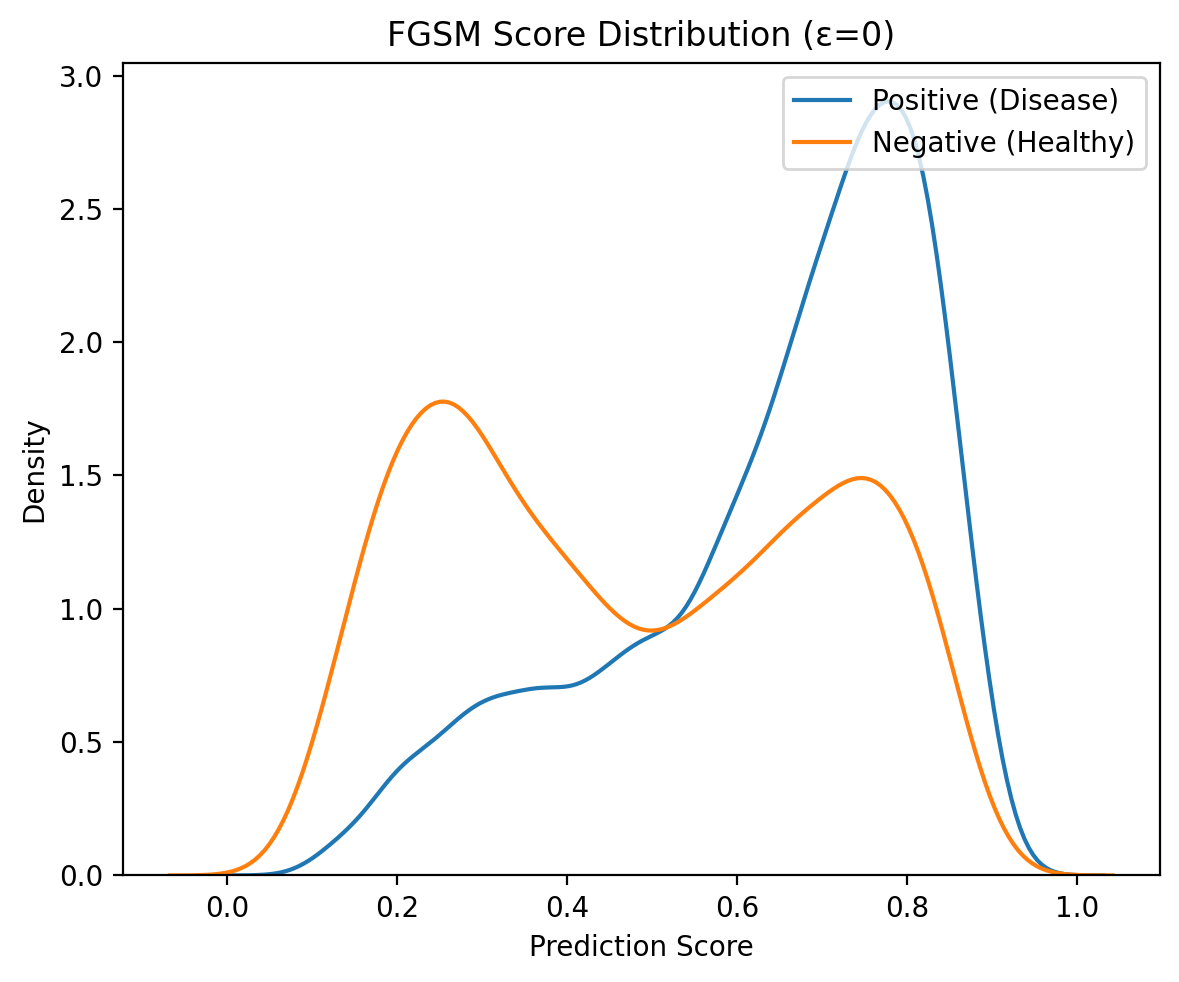
\includegraphics[width=\textwidth]{fgsm_score_eps0.png}
        \caption{Clean ($\epsilon=0$)}
    \end{subfigure}
    \hfill
    \begin{subfigure}[b]{0.32\textwidth}
        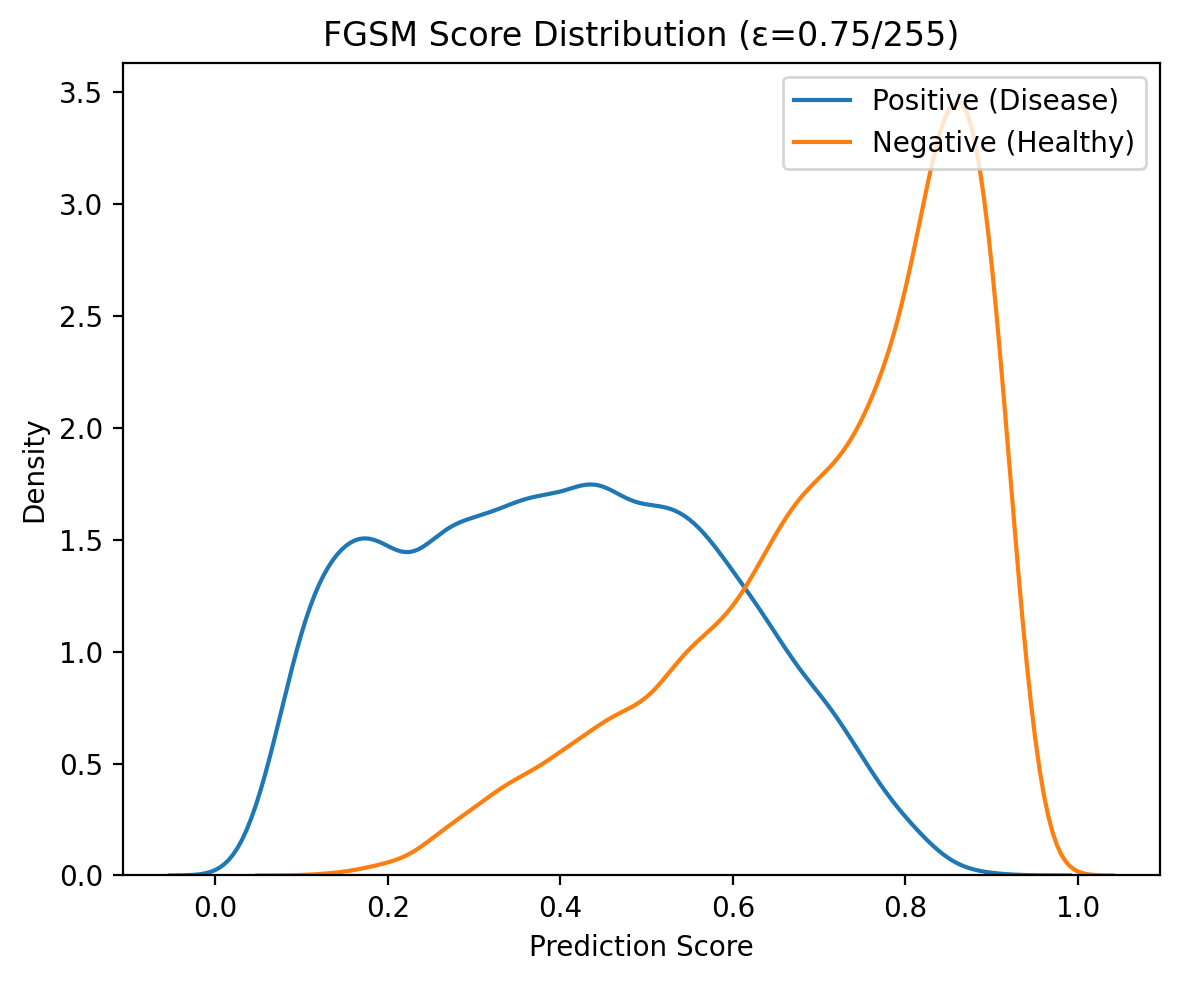
\includegraphics[width=\textwidth]{fgsm_score_eps0.0029411764705882353.png}
        \caption{$\epsilon=0.75/255$}
    \end{subfigure}
    \hfill
    \begin{subfigure}[b]{0.32\textwidth}
        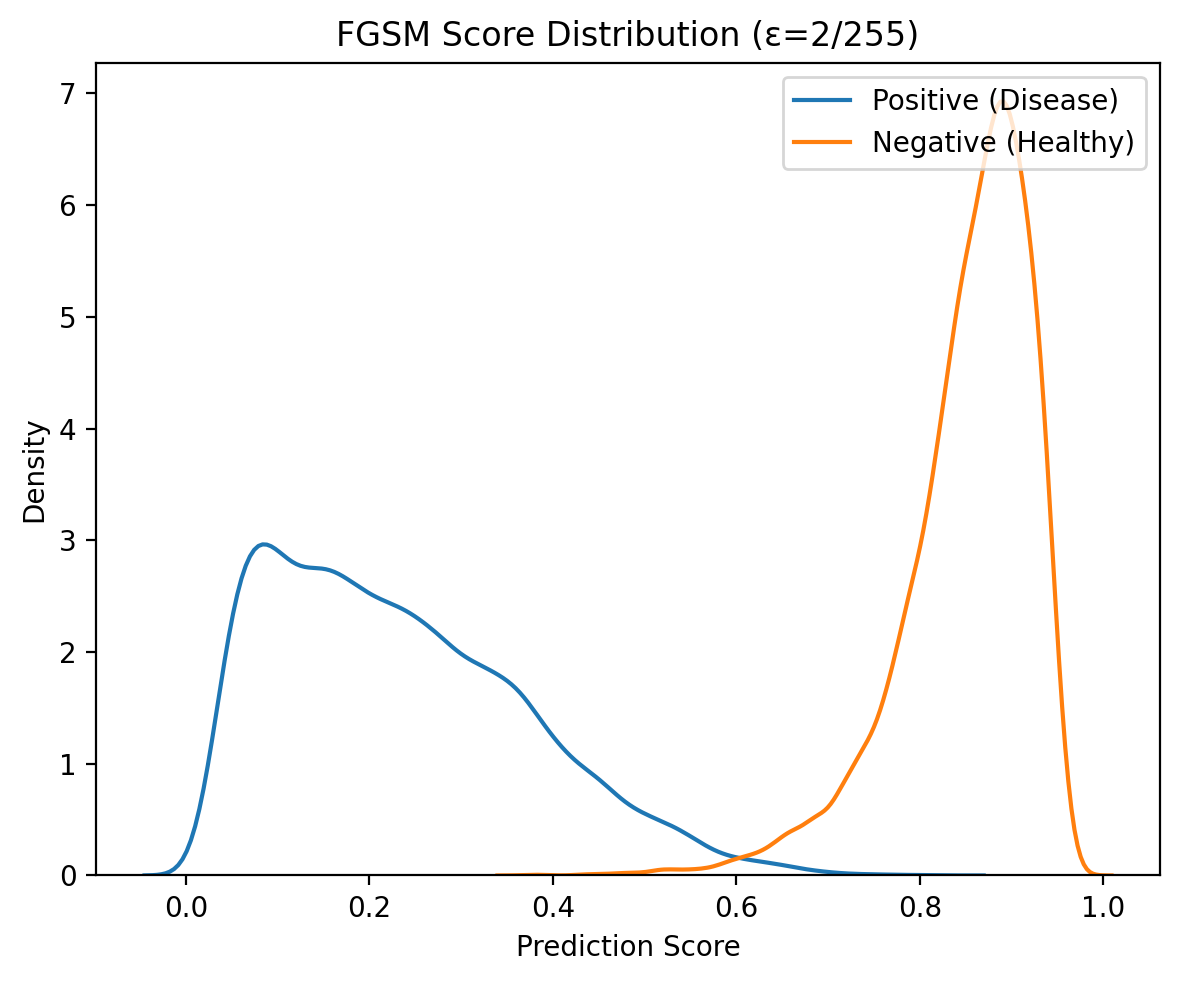
\includegraphics[width=\textwidth]{fgsm_score_eps0.00784313725490196.png}
        \caption{$\epsilon=2/255$}
    \end{subfigure}
    \caption{Score distributions under FGSM attack. In the clean case, positive and negative classes show separated distributions. Under attack, both distributions shift toward low scores, and separation is lost.}
    \label{fig:score_fgsm}
\end{figure}

In the clean case, the score distributions for positive and negative classes are reasonably separated, enabling classification. As perturbation increases, both distributions shift dramatically---positive cases receive low scores while negative cases cluster near zero. At $\epsilon=2/255$, the distributions completely overlap near zero, eliminating any basis for discrimination.

This analysis reveals that adversarial attacks work by systematically suppressing the model's confidence for the positive class, causing all samples to be classified as negative regardless of true label.

\subsubsection{Calibration Analysis}

Reliability diagrams assess whether the model's predicted probabilities match observed frequencies. A well-calibrated model should have points lying on the diagonal. Figure \ref{fig:reliability_fgsm} shows calibration degradation under attack.

\begin{figure}[htbp]
    \centering
    \begin{subfigure}[b]{0.32\textwidth}
        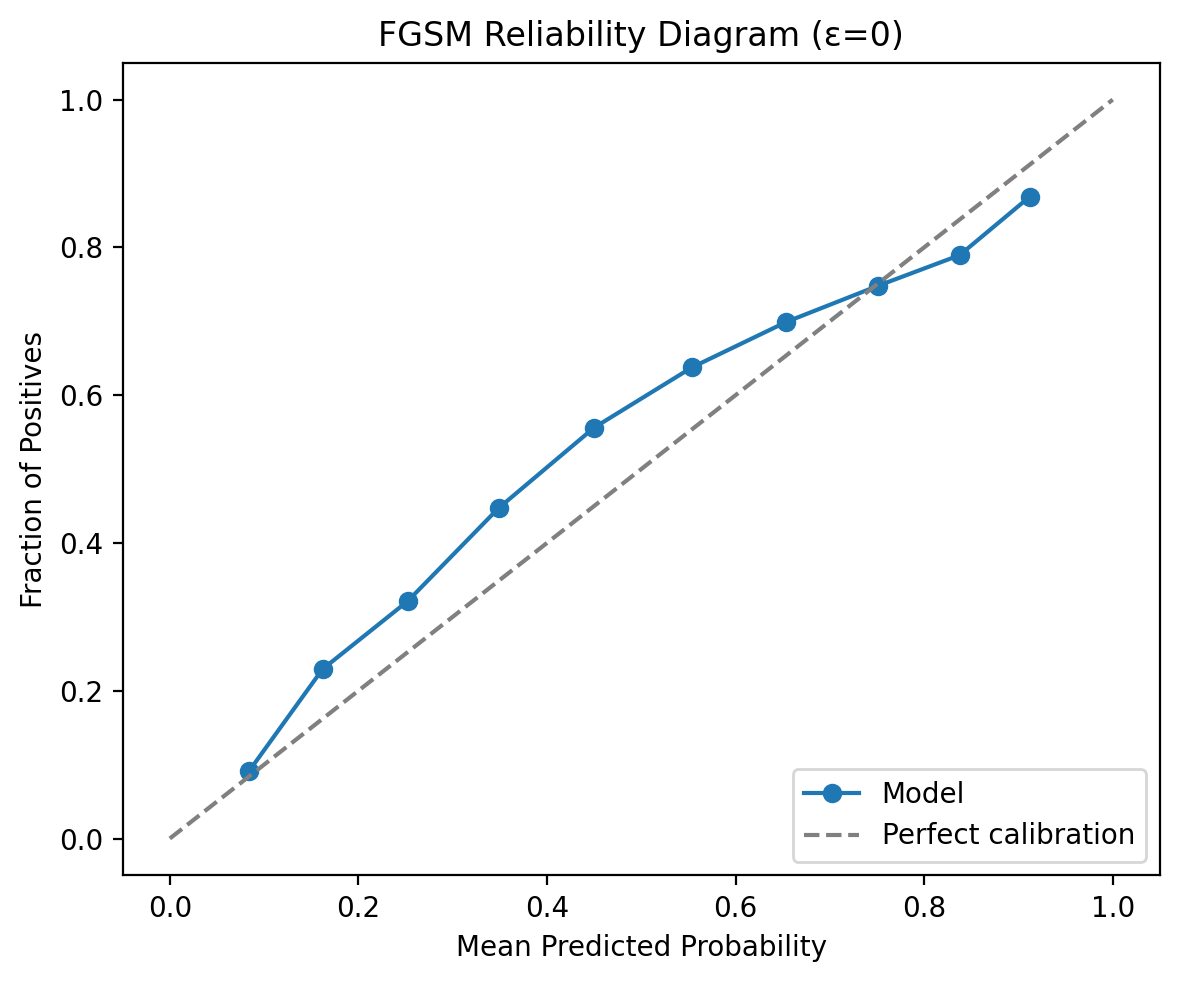
\includegraphics[width=\textwidth]{fgsm_reliability_eps0.png}
        \caption{Clean ($\epsilon=0$)}
    \end{subfigure}
    \hfill
    \begin{subfigure}[b]{0.32\textwidth}
        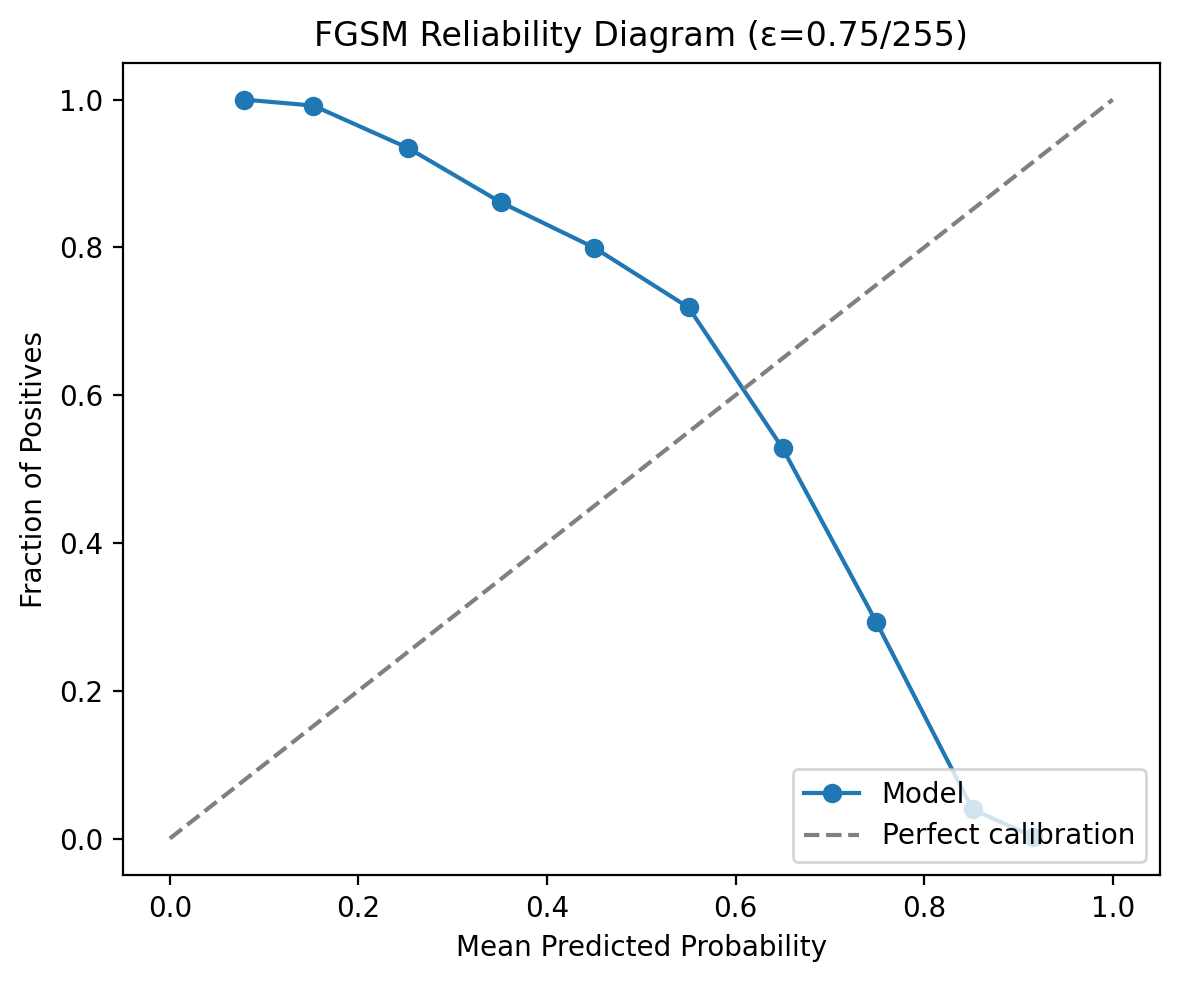
\includegraphics[width=\textwidth]{fgsm_reliability_eps0.0029411764705882353.png}
        \caption{$\epsilon=0.75/255$}
    \end{subfigure}
    \hfill
    \begin{subfigure}[b]{0.32\textwidth}
        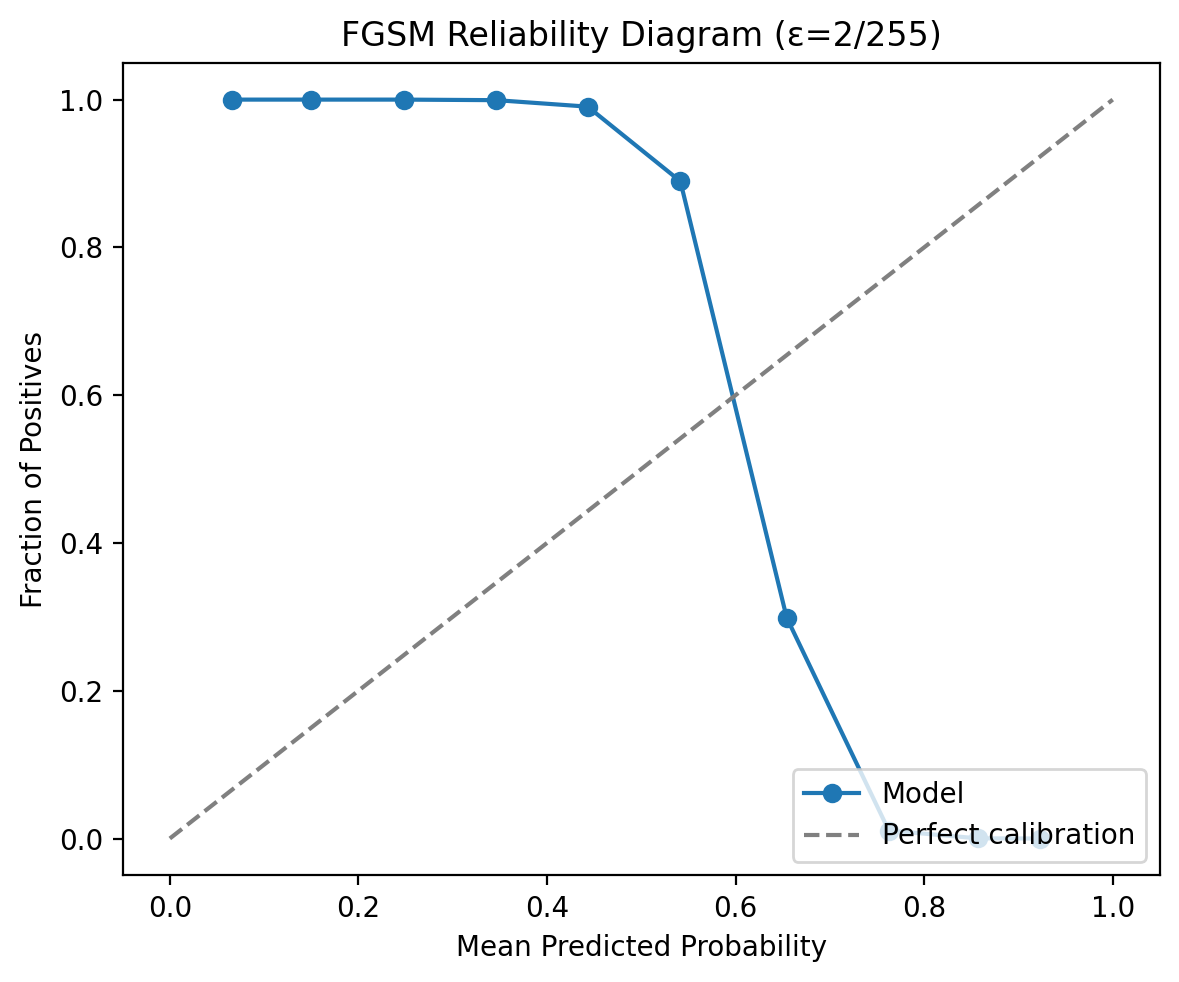
\includegraphics[width=\textwidth]{fgsm_reliability_eps0.00784313725490196.png}
        \caption{$\epsilon=2/255$}
    \end{subfigure}
    \caption{Reliability diagrams under FGSM attack. The clean model shows reasonable calibration. Under attack, calibration degrades severely---the model becomes both inaccurate and overconfident in its incorrect predictions.}
    \label{fig:reliability_fgsm}
\end{figure}

The calibration analysis reveals a dangerous pattern: adversarial attacks not only cause misclassification but also destroy the model's ability to express appropriate uncertainty. In clinical settings, a miscalibrated model that confidently makes incorrect predictions is more dangerous than one that correctly expresses uncertainty about difficult cases.

The Expected Calibration Error (ECE) increases from 0.126 in the clean case to 0.459 at $\epsilon=2/255$, indicating severe miscalibration. This finding suggests that uncertainty quantification and calibration-aware training may be important components of adversarial defense strategies for medical AI systems.

\subsection{Discussion}

\subsubsection{Severity of Vulnerability}

The experimental results reveal alarming vulnerability of the chest X-ray classification model. The complete collapse under imperceptible perturbations raises serious concerns about clinical deployment without robust defenses. At the largest tested perturbation of $\epsilon=2/255$, corresponding to a maximum per-pixel change of less than 1\% of the full intensity range, the model's accuracy drops to near zero. This level of perturbation is completely invisible to human observers, as demonstrated by our adversarial example visualizations.

The speed of accuracy degradation is particularly concerning. Even at $\epsilon=0.25/255$, a perturbation magnitude that corresponds to approximately 0.1\% of the pixel intensity range, accuracy drops by over 14 percentage points. This suggests that the model's decision boundaries are extremely irregular and that correctly classified examples exist in close proximity to adversarial regions. The fragility is not limited to a few edge cases but affects the entire test set systematically.

Several factors may contribute to this severe vulnerability:

\begin{itemize}[leftmargin=*]
    \item \textbf{High-dimensional input:} Medical images contain millions of pixels, providing attackers with enormous flexibility in crafting perturbations. The linear hypothesis suggests that adversarial vulnerability scales with input dimensionality, as the cumulative effect of small perturbations across many dimensions can produce large changes in output. A 224$\times$224 RGB image has over 150,000 dimensions, offering vast space for adversarial manipulation.
    
    \item \textbf{Transfer learning from ImageNet:} While ImageNet pre-training provides valuable low-level features, it may also transfer vulnerabilities. Features learned from natural images may include patterns that are predictive on ImageNet but irrelevant or misleading for medical imaging. These ``non-robust'' features could be exploited by adversarial attacks. The domain gap between colorful natural images and grayscale medical images may exacerbate this issue.
    
    \item \textbf{Label noise in training data:} The NLP-extracted labels in ChestX-ray14 contain significant noise, with disagreement rates of 10-20\% compared to expert annotations for some conditions. Training on noisy labels may prevent the model from learning sharp decision boundaries aligned with true disease features, creating regions of uncertainty that adversarial attacks can exploit.
    
    \item \textbf{Limited training data diversity:} Despite containing over 100,000 images, the training data comes from a single institution and may not cover the full diversity of chest X-ray presentations. Limited diversity may cause the model to rely on spurious correlations or shortcuts that do not generalize robustly.
    
    \item \textbf{Standard training objective:} The model was trained with standard cross-entropy loss to maximize clean accuracy, without any explicit robustness objectives. This training setup is known to produce models that are vulnerable to adversarial attacks, as there is no pressure to learn robust features or maintain smooth decision boundaries.
\end{itemize}

\subsubsection{FGSM versus PGD}

The comparison between FGSM and PGD attacks provides important insights for robustness evaluation and defense development. PGD consistently outperforms FGSM across all perturbation levels, confirming that iterative optimization finds more effective adversarial examples within the same perturbation budget.

The gap between FGSM and PGD is largest at intermediate epsilon values. At $\epsilon=0.75/255$, FGSM achieves 25.15\% accuracy while PGD achieves 16.76\%, a difference of 8.39 percentage points. This gap reflects PGD's ability to iteratively refine the perturbation direction, escaping suboptimal solutions that FGSM's single step may find. At very small epsilon values, both attacks have limited effectiveness, while at large epsilon values, both achieve near-complete success, narrowing the gap.
    
The practical implications of this comparison are significant for robustness evaluation. Evaluating robustness using only FGSM would overestimate the model's resilience to adversarial attacks. For accurate robustness assessment, stronger attacks like PGD should be used. Furthermore, if defenses are developed against FGSM alone, they may fail against PGD, providing a false sense of security. PGD serves as a more stringent test of adversarial robustness.
    
The computational cost difference between FGSM and PGD is also noteworthy. FGSM requires only a single forward and backward pass, while PGD with 10 iterations requires approximately 10 times the computation. For large-scale evaluation across multiple epsilon values and the entire test set, FGSM enables rapid assessment while PGD provides more thorough evaluation at higher computational cost. A practical approach is to use FGSM for initial screening and PGD for final robustness certification.
    
\subsubsection{Clinical Implications}
    
The demonstrated vulnerabilities have serious implications for the clinical deployment of AI-assisted chest X-ray interpretation systems:

\begin{itemize}[leftmargin=*]
    \item \textbf{Diagnostic integrity risk:} Malicious actors could potentially manipulate chest X-ray images to alter diagnostic outcomes. This could enable insurance fraud, where images are modified to show non-existent conditions to justify reimbursement for unnecessary procedures. Conversely, images could be modified to hide true pathology, potentially for malpractice concealment or insurance fraud. The imperceptibility of effective perturbations makes such manipulation extremely difficult to detect through visual inspection.

    \item \textbf{Trust and adoption challenges:} Knowledge of adversarial vulnerability may undermine clinician trust in AI diagnostic systems. If radiologists are aware that AI predictions can be manipulated by invisible perturbations, they may be reluctant to rely on AI assistance, reducing the potential benefits of these technologies. Building trust requires demonstrating robustness or developing detectable-manipulation mechanisms.

    \item \textbf{Regulatory implications:} As regulatory bodies become aware of adversarial vulnerabilities, robustness testing may become a requirement for medical AI approval. The FDA and other regulatory agencies are increasingly focused on AI safety and reliability. Developers may need to demonstrate adversarial robustness as part of the approval process, potentially requiring adversarial training or other defense mechanisms.

    \item \textbf{Security infrastructure requirements:} Deploying AI systems for medical imaging may require additional security measures to protect against adversarial attacks. This could include secure transmission channels to prevent image modification in transit, integrity verification mechanisms to detect tampering, and continuous monitoring for anomalous predictions that might indicate attack attempts.

    \item \textbf{Workflow integration considerations:} The integration of AI predictions into clinical workflows must account for adversarial vulnerability. AI systems might be positioned as decision support tools requiring human verification rather than autonomous diagnostic agents. Radiologists should be trained to recognize situations where AI predictions should be viewed with particular skepticism.
\end{itemize}

\subsubsection{Comparison with Related Work}

Our findings align with and extend previous research on adversarial robustness in medical imaging. The severe vulnerability we observe is consistent with reports from Finlayson et al., Ma et al., and other researchers who have demonstrated successful adversarial attacks on medical AI systems. However, our study provides more comprehensive quantitative characterization across multiple perturbation levels and attack methods.

The accuracy-epsilon curves we generate provide fine-grained robustness profiles that complement the attack success rates reported in previous studies. By evaluating at six epsilon values with both FGSM and PGD, we characterize the full spectrum of vulnerability from imperceptible to barely visible perturbations.

Our Grad-CAM analysis adds interpretability insights that have been less explored in medical imaging adversarial robustness research. The observation that adversarial perturbations fundamentally disrupt attention patterns, rather than merely shifting classification thresholds, suggests that attacks affect the model's feature extraction process at a deep level.

\subsubsection{Limitations of This Study}

Several limitations of this study should be acknowledged when interpreting results:

\begin{itemize}[leftmargin=*]
    \item \textbf{Single model architecture:} We evaluated only ResNet-18. Other architectures, such as DenseNet or Vision Transformers, may have different vulnerability profiles. Architectural variations in depth, width, skip connections, and attention mechanisms could affect robustness.
    
    \item \textbf{White-box threat model:} All attacks assume complete knowledge of the model, representing the strongest possible adversary. Black-box attacks, where the attacker has limited or no model access, would likely be less effective. Our results represent worst-case vulnerabilities.
    
    \item \textbf{$L_\infty$ perturbation norm:} We focused on $L_\infty$-bounded perturbations. Other perturbation types, such as $L_2$-bounded or sparse perturbations, may yield different robustness profiles. The choice of norm affects both attack effectiveness and perturbation perceptibility.
    
    \item \textbf{No defense evaluation:} We did not evaluate defense mechanisms such as adversarial training, input preprocessing, or certified defenses. The baseline model represents standard practice without robustness enhancements.
    
    \item \textbf{Single dataset:} Results are based on NIH ChestX-ray14. Generalization to other datasets, imaging modalities, or clinical populations requires additional validation.
\end{itemize}

%==============================================================================
% SECTION 6: CONCLUSIONS AND FUTURE WORK
%==============================================================================
\section{Conclusions and Future Work}
\label{sec:conclusions}

\subsection{Summary of Findings}

This project presents a comprehensive evaluation of adversarial robustness for deep learning-based chest X-ray classification. Through systematic experimentation across multiple attack methods and perturbation levels, we have characterized the vulnerability of a representative medical image classification model and provided insights into the mechanisms by which adversarial attacks succeed. Our key findings include:

\begin{enumerate}[leftmargin=*]
    \item \textbf{Severe Vulnerability:} The ResNet-18 model shows extreme vulnerability to gradient-based attacks, with accuracy dropping from 68.51\% to 2.80\% under FGSM and to 0.08\% under PGD at $\epsilon=2/255$. This represents near-complete loss of discriminative ability under perturbations that are completely invisible to human observers. The model, which achieves reasonable performance on clean data, becomes essentially useless under adversarial attack.
    
    \item \textbf{Imperceptible Perturbations Suffice:} Even the smallest tested perturbation ($\epsilon=0.25/255$), corresponding to approximately 0.1\% of the pixel intensity range, causes significant accuracy degradation of over 14\%. This demonstrates that clinically harmful attacks do not require large, detectable modifications. An attacker needs only imperceptible changes to flip diagnostic predictions, with potentially serious consequences for patient care.
    
    \item \textbf{PGD Superiority:} Iterative PGD attacks consistently achieve greater degradation than single-step FGSM, with the gap most pronounced at intermediate perturbation levels. This finding has important implications for robustness evaluation: using only FGSM would overestimate model robustness. PGD should be the standard for rigorous adversarial evaluation, despite its higher computational cost.
    
    \item \textbf{Attention Disruption:} Grad-CAM analysis reveals that adversarial perturbations fundamentally alter model attention patterns, shifting focus away from diagnostically relevant regions. Rather than merely pushing predictions across decision boundaries, attacks appear to disrupt the feature extraction process at a fundamental level. The model attends to different image regions under attack, suggesting that perturbations create spurious features or mask genuine disease indicators.
    
    \item \textbf{Calibration Failure:} Adversarial examples cause severe calibration degradation, with the model producing overconfident incorrect predictions. The Expected Calibration Error (ECE) increases dramatically under attack, indicating that predicted probabilities become unreliable indicators of true uncertainty. This is particularly dangerous in clinical settings where probability estimates inform treatment decisions.
    
    \item \textbf{Systematic Prediction Shift:} Analysis of confusion matrices and score distributions reveals that attacks systematically suppress positive class predictions, causing the model to classify nearly all images as negative (healthy) regardless of true label. This pattern suggests that attacks exploit asymmetries in the model's decision-making, potentially related to class imbalance in training data or differences in feature representations between classes.
\end{enumerate}

\subsection{Contributions}

This project makes several contributions to the field of medical AI security and adversarial robustness:

\begin{itemize}[leftmargin=*]
    \item \textbf{Comprehensive Empirical Study:} We provide a thorough empirical evaluation with 25,583 test images across six perturbation levels and two attack methods, generating robustness curves that characterize vulnerability across the full perturbation spectrum. This represents one of the most comprehensive evaluations of adversarial robustness in medical image classification to date.
    
    \item \textbf{Integrated Evaluation Framework:} We develop an evaluation framework that combines accuracy metrics, calibration analysis, and visual interpretability through Grad-CAM. This multi-faceted approach provides a more complete picture of how adversarial attacks affect model behavior than accuracy metrics alone. The framework can be applied to evaluate robustness of other medical imaging models.
    
    \item \textbf{Open-Source Implementation:} All code for attack implementation, evaluation, and visualization is made available as open-source software. This enables other researchers to reproduce our results, apply our evaluation framework to their own models, and extend our work. Reproducibility is essential for scientific progress in adversarial robustness research.
    
    \item \textbf{Quantitative Attack Comparison:} We provide systematic comparison of FGSM and PGD effectiveness, demonstrating the importance of using strong attacks for robustness evaluation. The quantitative results can inform choices about computational budget allocation in future robustness studies.
    
    \item \textbf{Visual Analysis of Attack Mechanisms:} Through Grad-CAM visualization, we provide qualitative insights into how adversarial attacks affect model attention and feature extraction. These visualizations make the abstract concept of adversarial vulnerability more tangible and may inspire new defense strategies focused on maintaining robust attention patterns.
    
    \item \textbf{Clinical Relevance Analysis:} We contextualize our technical findings in terms of clinical implications, discussing potential attack scenarios, regulatory considerations, and workflow integration challenges. This bridges the gap between technical adversarial robustness research and practical medical AI deployment concerns.
\end{itemize}

\subsection{Limitations}

This study has several limitations that should be considered when interpreting and generalizing results:

\begin{enumerate}[leftmargin=*]
    \item \textbf{Single Architecture:} Only ResNet-18 was evaluated. Other architectures, including deeper ResNets, DenseNets, EfficientNets, and Vision Transformers, may exhibit different vulnerability profiles. Architectural differences in depth, skip connections, attention mechanisms, and normalization could affect adversarial robustness. Broader architectural comparison would strengthen generalizability claims.
    
    \item \textbf{Binary Classification:} The binary formulation (disease vs. no finding) simplifies the multi-label nature of chest X-ray diagnosis. Real clinical workflows often require distinguishing between specific diseases, each with potentially different adversarial vulnerability. Multi-label classification introduces additional complexity in both attack formulation and evaluation.
    
    \item \textbf{White-box Threat Model:} All attacks assume complete knowledge of the model, including architecture and parameters. This represents the strongest possible adversary but may overestimate practical risk. Black-box attacks, where the attacker has limited or no model access, would likely be less effective but are more realistic in many deployment scenarios. Transfer attacks, using surrogate models to generate adversarial examples, would provide intermediate threat assessment.
    
    \item \textbf{No Defense Evaluation:} We characterize vulnerability but do not evaluate defense mechanisms. Understanding baseline vulnerability is a necessary first step, but practical deployment requires effective defenses. Future work should evaluate adversarial training, certified defenses, and detection methods on this benchmark.
    
    \item \textbf{Single Dataset:} Results are based on NIH ChestX-ray14 from a single institution. Generalization to other datasets (CheXpert, MIMIC-CXR), imaging modalities (CT, MRI), anatomical regions, and clinical populations requires additional validation. Domain shift between datasets could affect both clean accuracy and adversarial robustness.
    
    \item \textbf{Digital Perturbations Only:} We consider only digital perturbations applied directly to pixel values. Physical adversarial attacks, where perturbations must be realized through physical means (printed patches, modified equipment settings), face additional constraints and may be less effective. However, physical attacks represent a different and potentially more realistic threat model.
\end{enumerate}

\subsection{Future Work}

Based on our findings and identified limitations, we propose several directions for future research:

\begin{itemize}[leftmargin=*]
    \item \textbf{Defense Evaluation and Development:} The most pressing need is for effective defenses against adversarial attacks in medical imaging. Future work should evaluate established defenses such as adversarial training on this benchmark and develop new defenses specifically designed for medical imaging characteristics. Adversarial training, while effective in natural image domains, has not been extensively studied for medical images and may require adaptation to address the unique properties of medical imaging data.
    
    \item \textbf{Certified Defenses:} Investigating certified defenses that provide provable robustness guarantees is an important direction. While current certified methods achieve limited practical robustness, they offer formal guarantees that may be particularly valuable in safety-critical medical applications. Randomized smoothing and other certification approaches should be evaluated for medical imaging.
    
    \item \textbf{Detection Methods:} Developing methods to detect adversarially manipulated medical images is a complementary approach to robust classification. Detection methods could flag suspicious images for human review, providing a safety net even when classification robustness cannot be guaranteed. Research should investigate statistical detection methods, separate detector networks, and consistency-based approaches.
    
    \item \textbf{Black-box and Transfer Attacks:} Evaluating robustness under more realistic black-box threat models is important for understanding practical risk. Future work should investigate transfer attacks using surrogate models, query-based attacks, and decision-based attacks that do not require gradient access.
    
    \item \textbf{Multi-label and Multi-class Evaluation:} Extending robustness evaluation to multi-label chest X-ray classification and other multi-class medical imaging tasks would provide more comprehensive understanding of adversarial vulnerability across clinical applications.
    
    \item \textbf{Architectural Comparison:} Systematic comparison of adversarial robustness across different neural network architectures would identify architectural features that enhance or reduce vulnerability. This could guide the selection and design of architectures for robust medical AI systems.
    
    \item \textbf{Clinical Workflow Integration:} Investigating how robustness testing and adversarial defenses can be practically integrated into clinical AI deployment pipelines is essential for translating research advances into improved patient safety. This includes developing standards for robustness certification, designing human-AI interaction protocols that account for adversarial vulnerability, and creating tools for continuous monitoring of deployed systems.
    
    \item \textbf{Regulatory Framework Development:} Working with regulatory bodies to develop frameworks for assessing and certifying adversarial robustness of medical AI devices would advance the field toward practical deployment. This requires translating technical robustness metrics into clinically meaningful safety standards.
\end{itemize}

\subsection{Concluding Remarks}

As medical AI systems become increasingly integrated into clinical workflows, ensuring their robustness against adversarial manipulation is essential for patient safety. The deployment of AI systems that can be fooled by imperceptible image modifications poses unacceptable risks in settings where diagnostic errors can directly harm patients.

This project demonstrates that current deep learning models for chest X-ray classification are highly vulnerable to imperceptible perturbations, highlighting the critical need for robust defenses before clinical deployment. A model that achieves 68.51\% accuracy on clean test data---reasonable performance for this challenging task---collapses to near-zero accuracy under adversarial attack. This gap between clean and adversarial performance represents a fundamental reliability failure that must be addressed.

The findings underscore that achieving high accuracy on clean test data is insufficient for clinical safety; models must also demonstrate resilience to adversarial manipulation. Standard machine learning evaluation practices, which focus exclusively on clean data performance, fail to capture this critical dimension of model reliability. Adversarial robustness evaluation should become a standard component of medical AI development and validation.

We hope this work contributes to the growing awareness of adversarial robustness in medical AI and provides useful benchmarks and tools for future research. The comprehensive evaluation framework, quantitative results, and visual analyses presented here can serve as references for researchers and practitioners working to develop safer medical AI systems.

The path from vulnerable research prototypes to robust clinical tools will require sustained effort across multiple fronts: developing effective defenses, creating appropriate evaluation standards, establishing regulatory frameworks, and building clinical workflows that appropriately account for AI limitations. While the challenges are significant, addressing them is essential for realizing the potential benefits of AI in healthcare while protecting patient safety.

% References
\newpage
\section*{References}
\addcontentsline{toc}{section}{References}
\printbibliography[heading=none]

% Appendices
\newpage
\begin{appendices}
    \section{Appendices}
    \label{sec:appendices}
    
    This appendix contains supplementary materials submitted during the project lifecycle.
    
    \section{Risk Assessment}
    \label{app:risk}
    
    A formal risk assessment was completed at the start of the project. The primary risks identified include data privacy considerations, potential misuse of adversarial attack research, and clinical misinterpretation of results. The complete risk assessment form is attached below.
    
    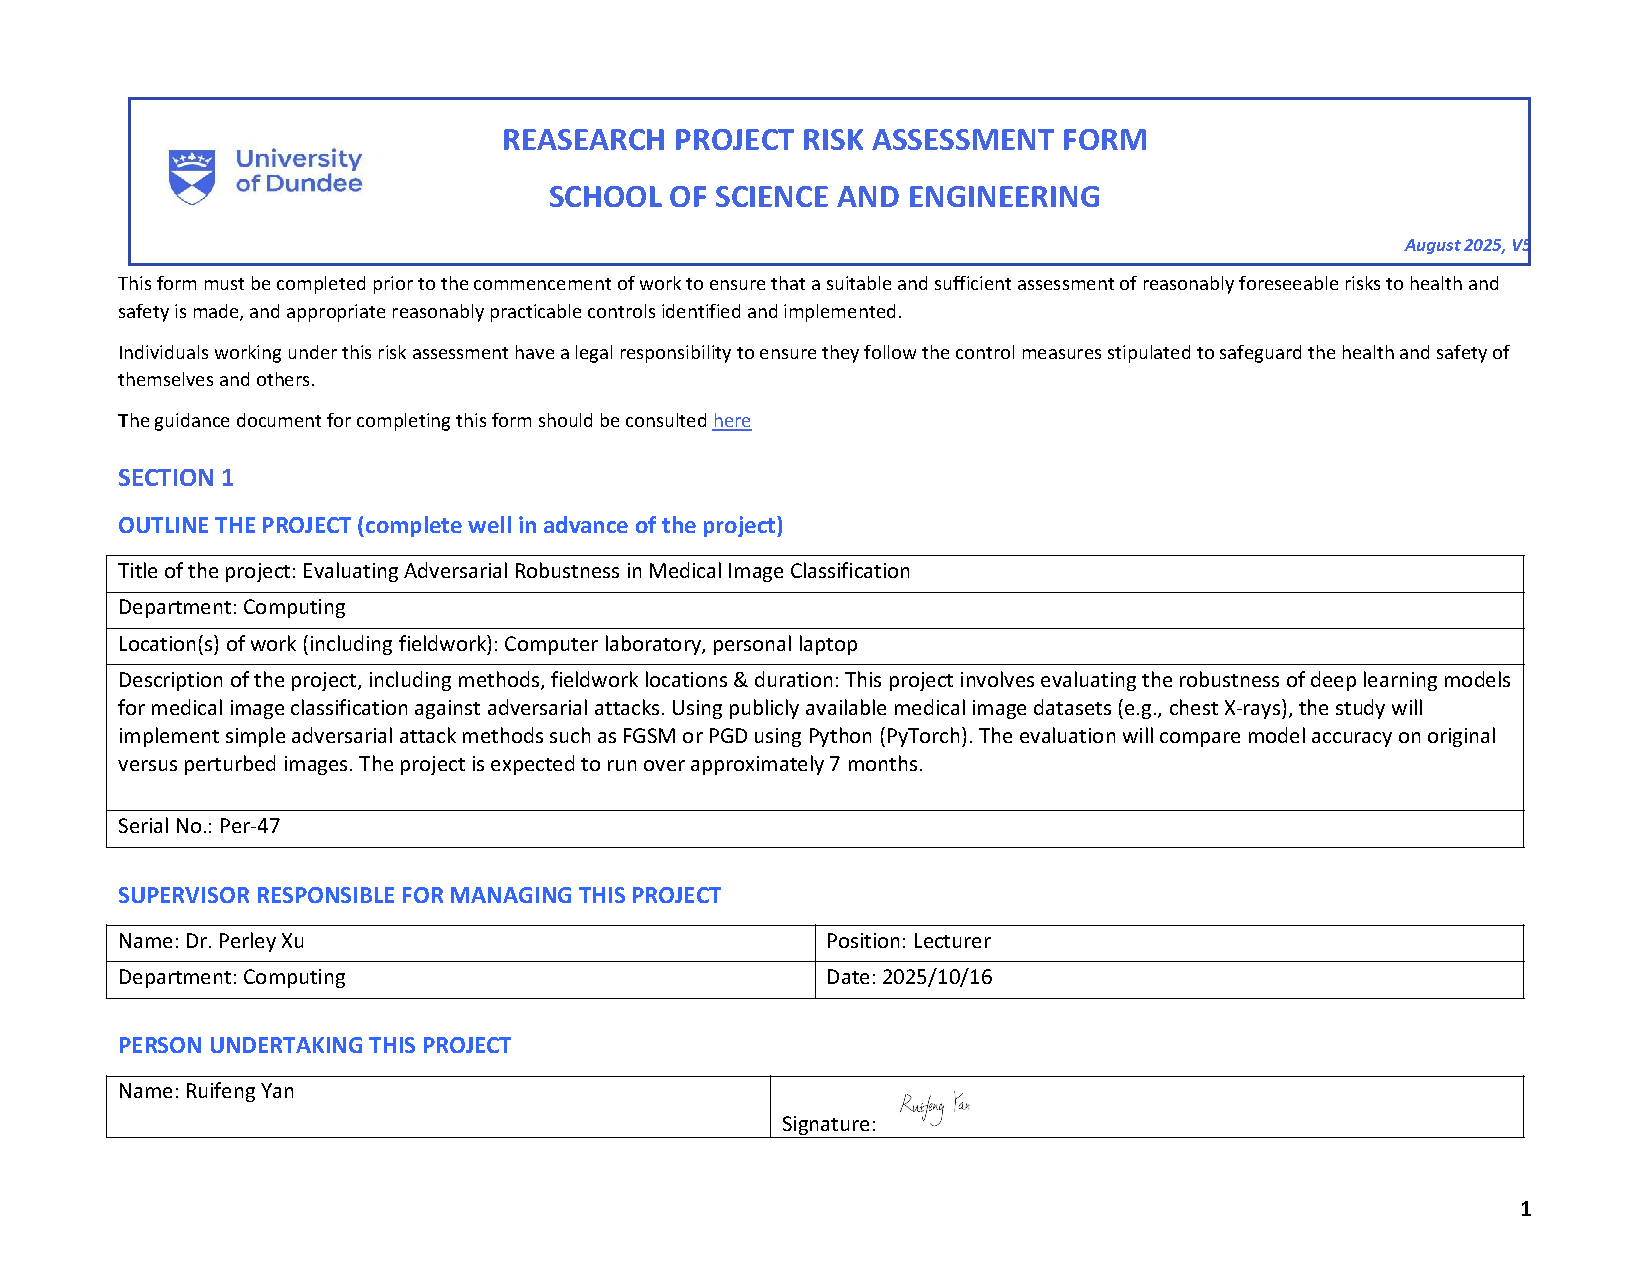
\includepdf[pages=-,pagecommand={\thispagestyle{plain}},scale=0.85]{media/SSEN Student Project Risk Assessment_RuifengYan.pdf}
    
    \section{Ethics Form}
    \label{app:ethics}
    
    The DIICSU Honours Project Ethics Form was completed and submitted. This project uses only publicly available, de-identified data (NIH ChestX-ray14) and does not involve human subjects research. No additional ethics approval was required. The complete ethics form is attached below.
    
    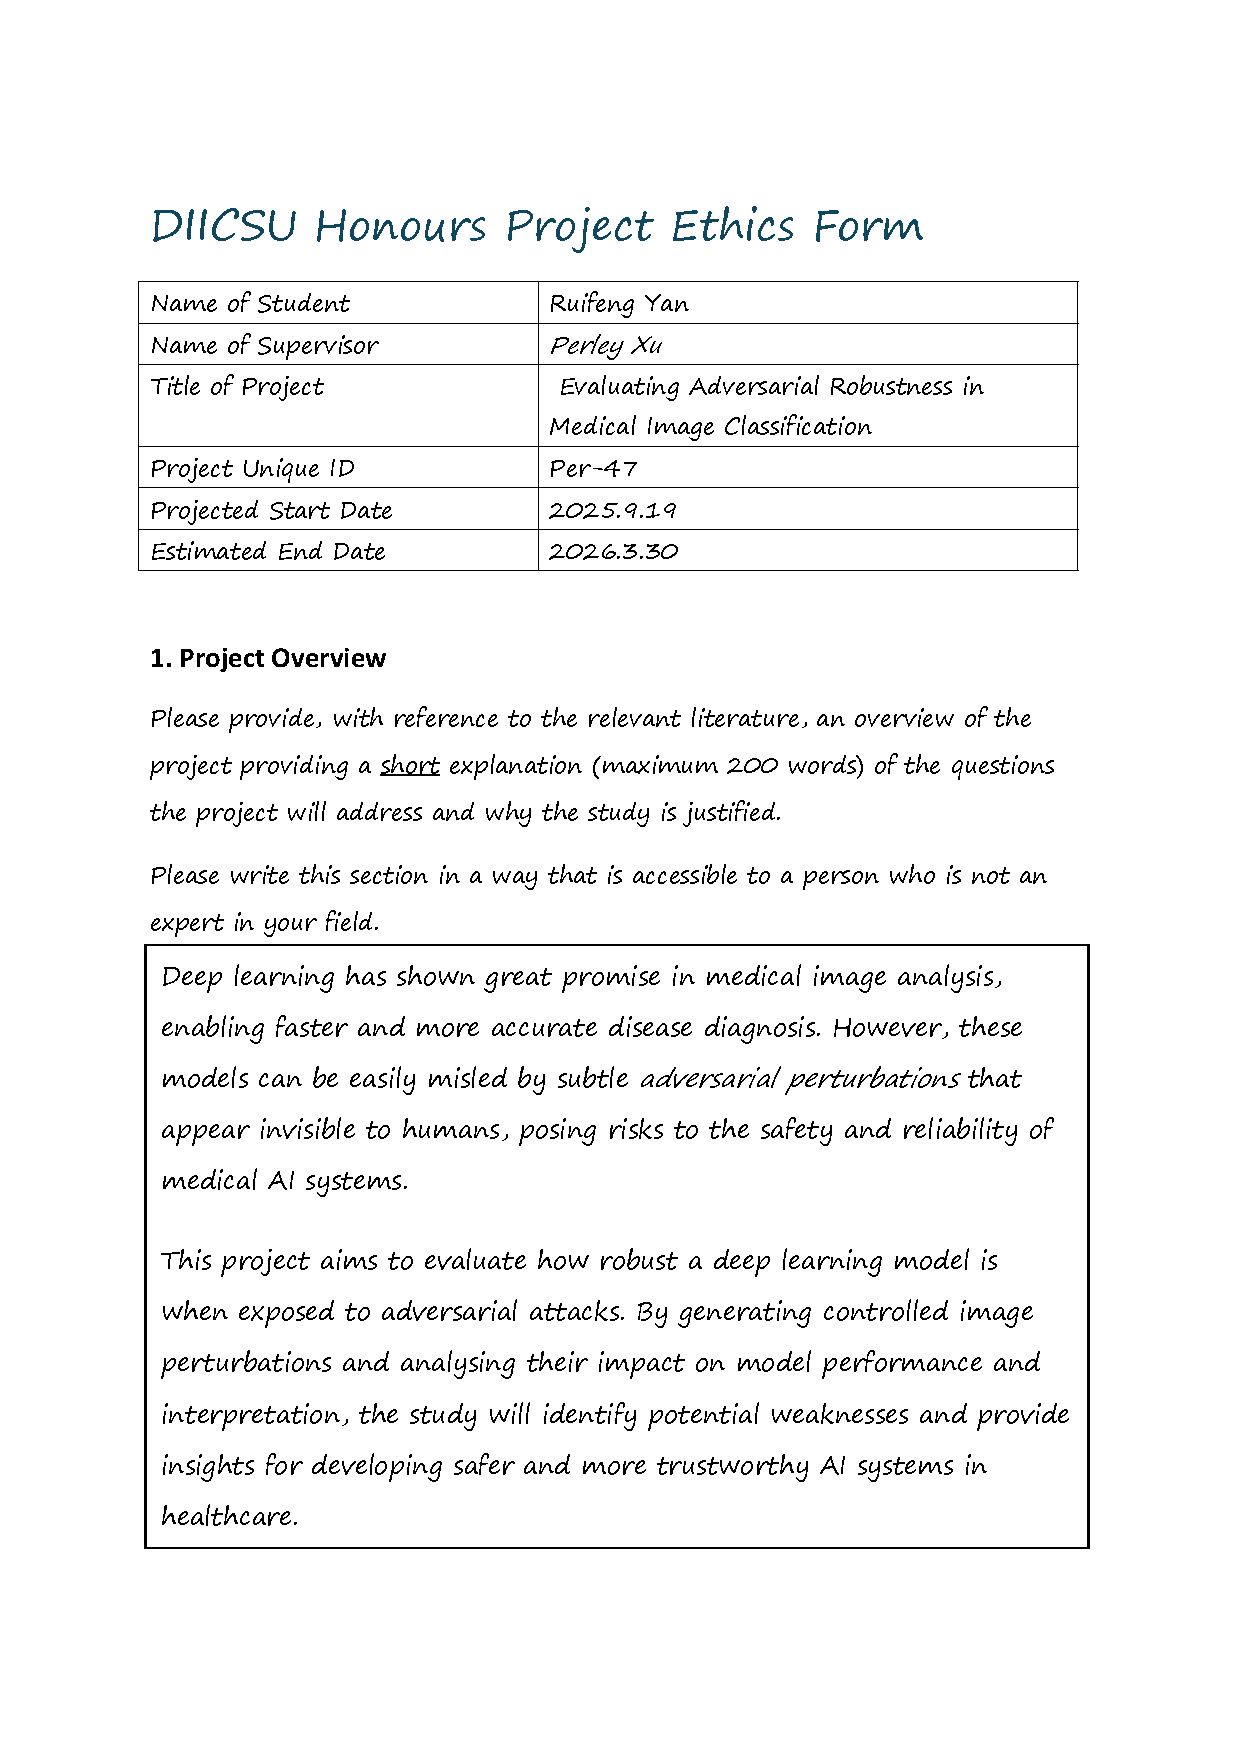
\includepdf[pages=-,pagecommand={\thispagestyle{plain}},scale=0.85]{media/DIICSU Honours Project Ethics Form——Ruifeng Yan.pdf}
    
    \section{Project Plan and Gantt Chart}
    \label{app:gantt}
    
    A detailed project plan was created using a Gantt chart. The project was completed in the following phases: Literature Review (Weeks 1-5), Prototype Experimentation (Weeks 6-10), Dataset Preparation (Weeks 11-13), Model Training (Weeks 14-15), Attack Implementation (Weeks 16-17), Robustness Evaluation (Weeks 18-20), Visualization and Analysis (Weeks 21-23), Report Writing (Weeks 24-26), and Contingency Buffer (Weeks 27-28). The complete Gantt chart is attached below.
    
    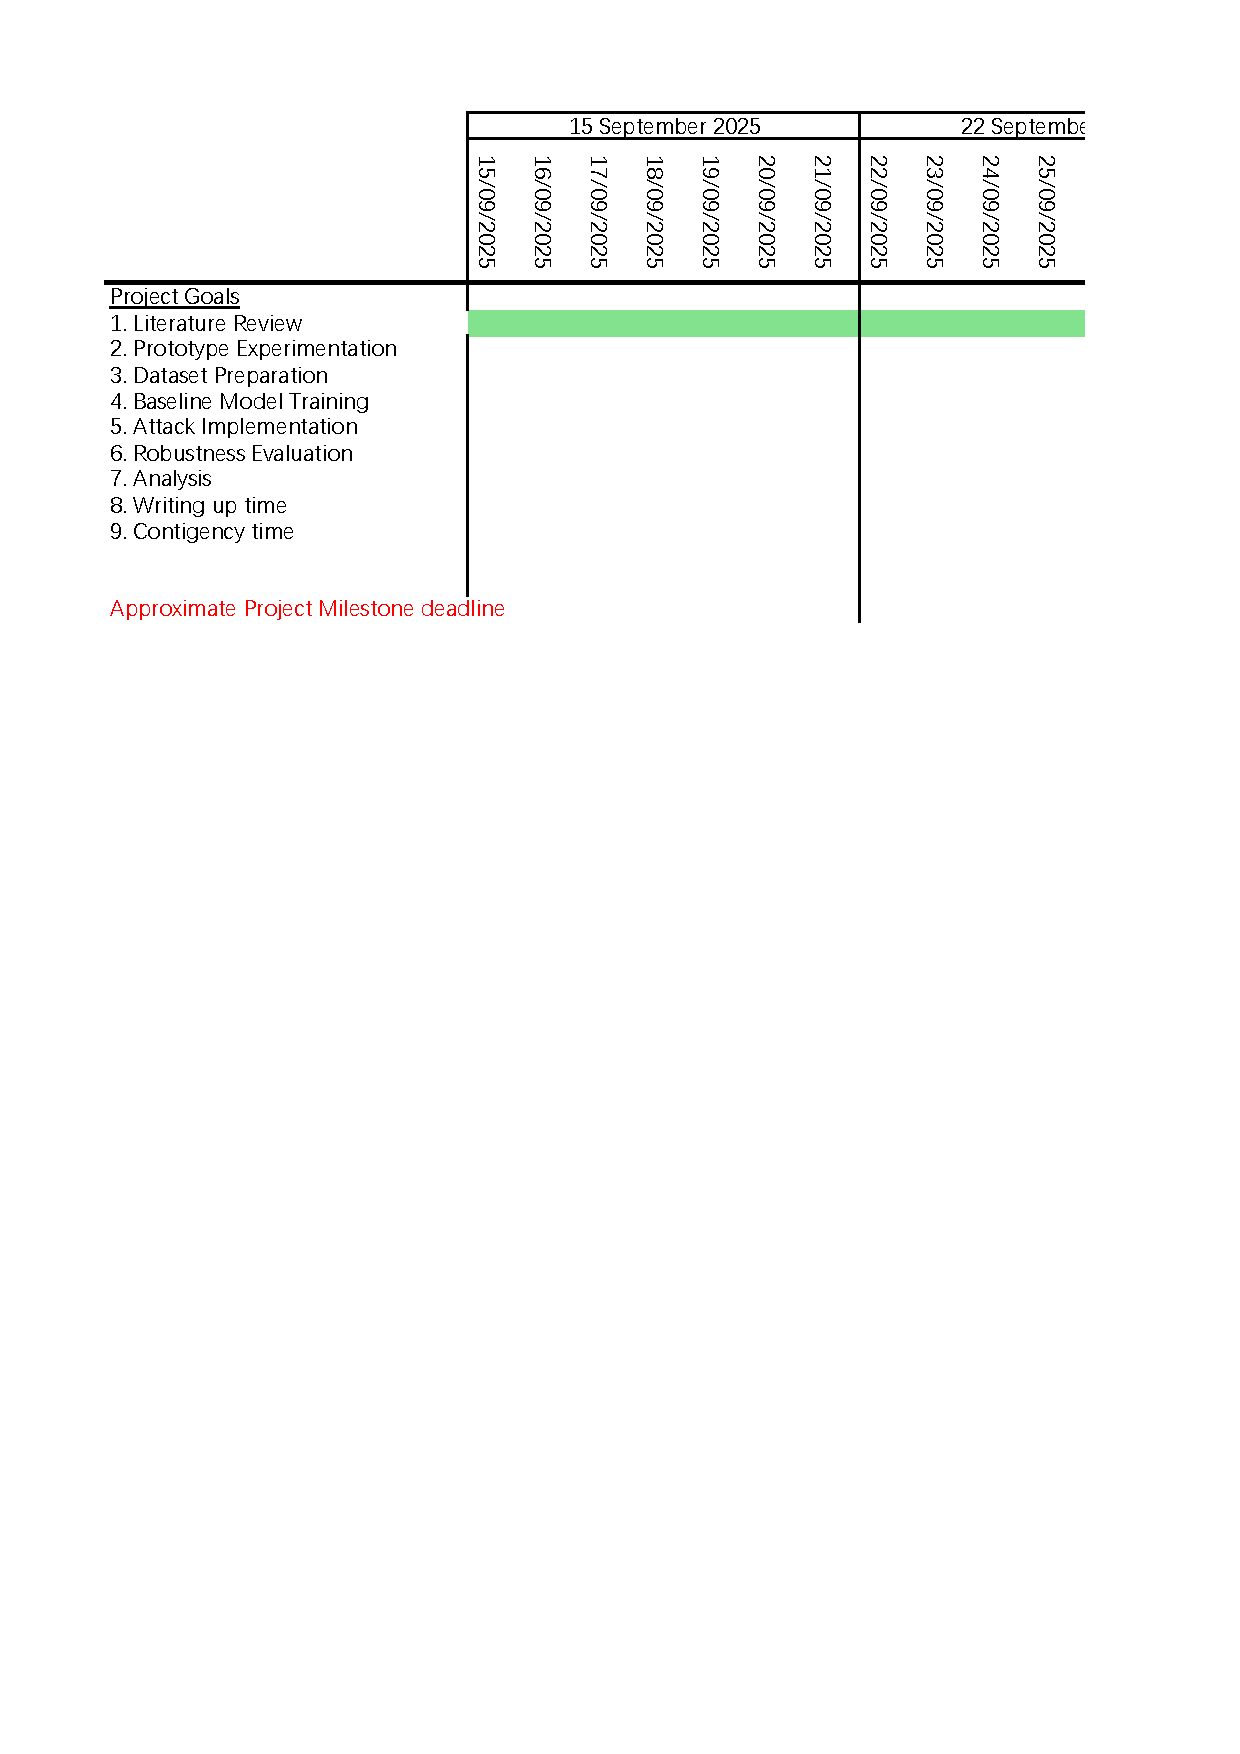
\includepdf[pages=-,pagecommand={\thispagestyle{plain}},scale=0.85]{media/Project Gantt Chart -Ruifeng Yan.pdf}
    
    \section{Midterm Report}
    \label{app:midterm}
    
    A midterm report was submitted documenting progress at the project's midpoint. The report detailed project aims, objectives, SMART goals, summary of completed work including literature review, environment setup, prototype experimentation, initial results, and plan for remaining work. The full midterm report is attached below.
    
    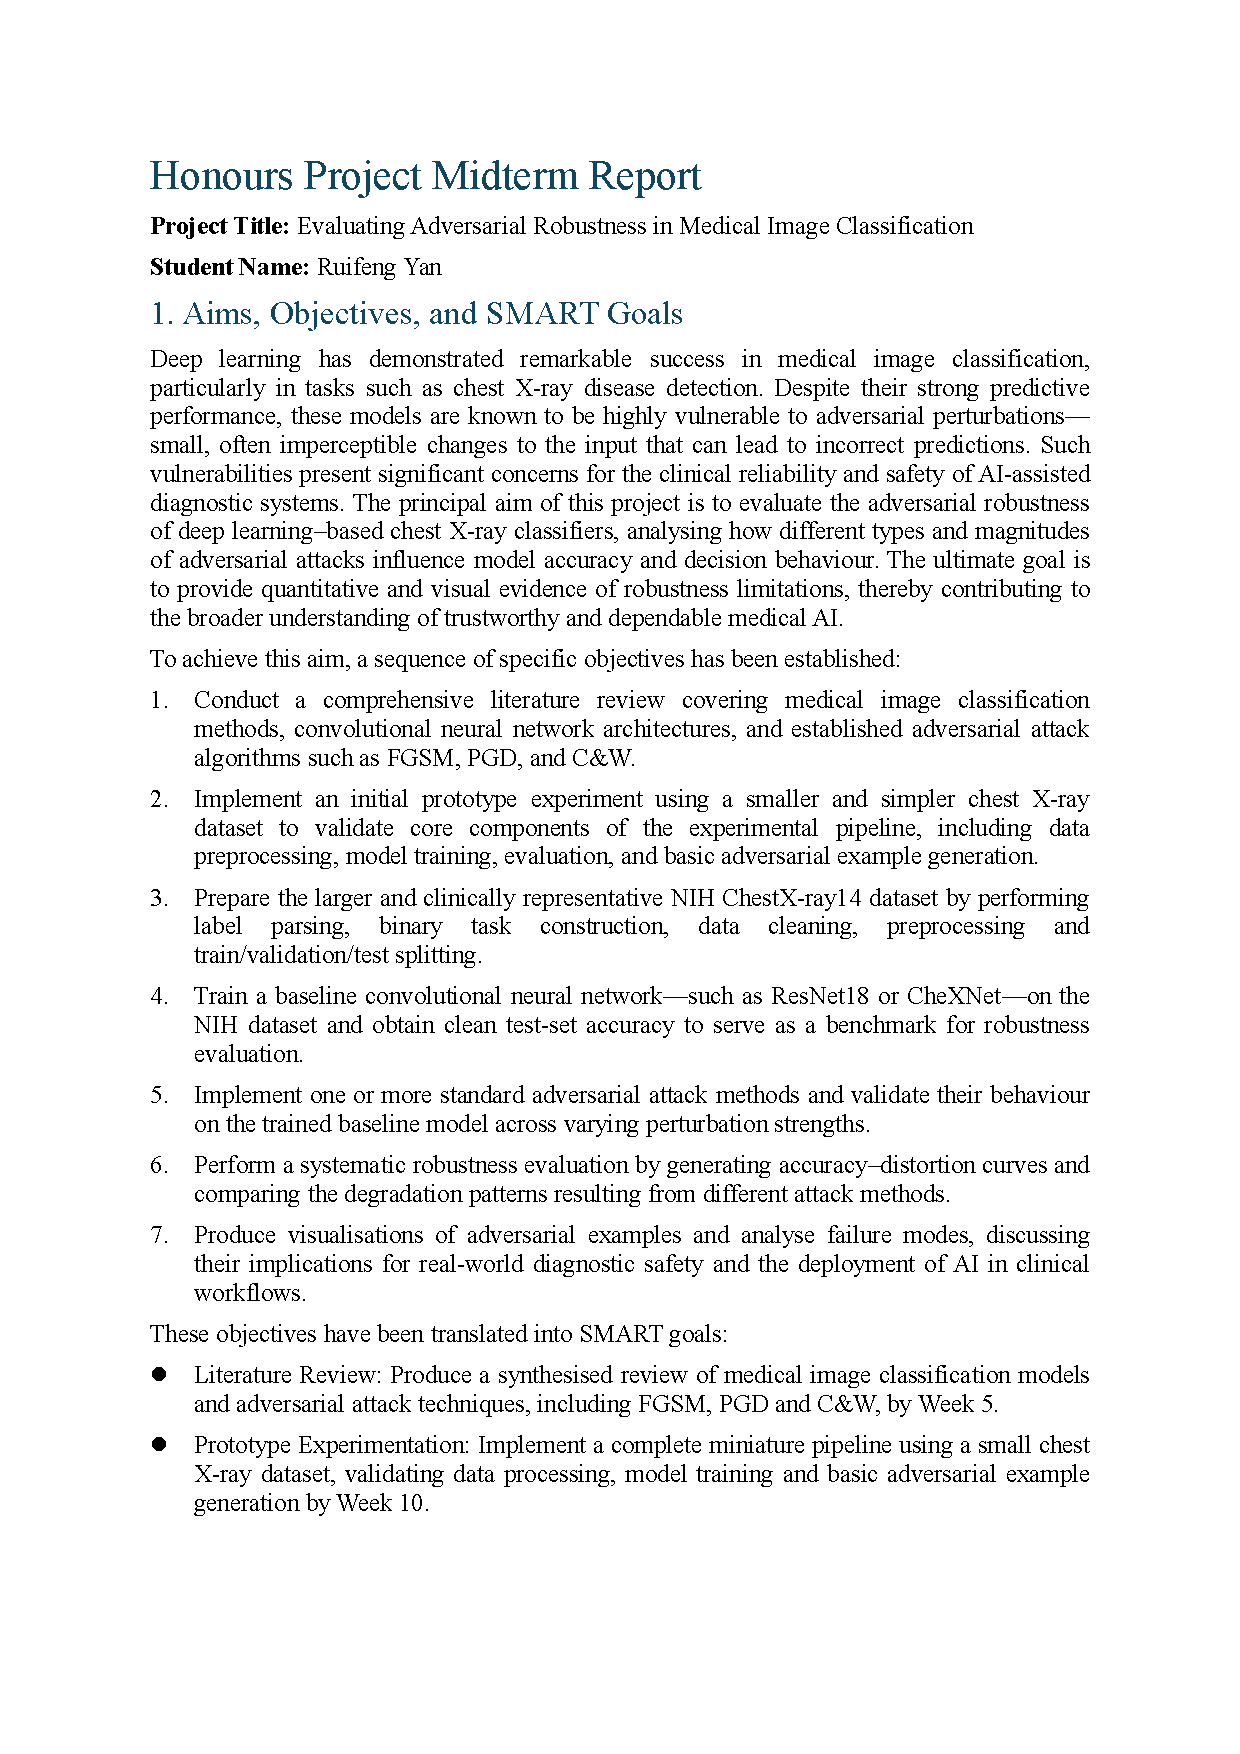
\includepdf[pages=-,pagecommand={\thispagestyle{plain}},scale=0.85]{media/Honours Project Midterm Report - Ruifeng Yan.pdf}
    
    \section{AI Declaration}
    \label{app:ai}
    
    The AI Declaration form documents the use of AI tools in this project. The following AI tools were used: GitHub Copilot for code completion and debugging suggestions, and ChatGPT/Claude for clarifying technical concepts and debugging assistance. All AI-generated content was reviewed, verified, and modified as necessary. The core research methodology, experimental design, and analysis were conducted independently. The complete AI Declaration form is attached below.
    
    
\includepdf[pages=-,pagecommand={\thispagestyle{plain}},scale=0.85]{media/AI Declaration.pdf}
    
    \section{Supervisor Meeting Minutes}
    \label{app:meetings}
    
    Regular meetings were held with the supervisor throughout the project. Key discussion points included initial project scoping and objectives, dataset selection and preprocessing approach, attack method selection, evaluation metric design, results interpretation and presentation, and report structure. Meeting minutes and presentation materials are available at:
    
    \url{https://dmail-my.sharepoint.com/:f:/g/personal/2542795_dundee_ac_uk/IgBBE2TdTCKDQYA3g-QGS61bAaCqYINiPJrrCKetxe2VaGo?e=4MI5Hr}
    
    \section{Source Code}
    \label{app:code}
    
    The complete source code for this project, including attack implementations, evaluation scripts, and visualization tools, is publicly available on GitHub:
    
    \url{https://github.com/yrf123456/chest-xray-adversarial-robustness}
    
    The repository contains:
    \begin{itemize}
        \item FGSM and PGD attack implementations
        \item Robustness evaluation pipeline
        \item Grad-CAM visualization tools
        \item Model training scripts
        \item Dataset preprocessing utilities
        \item All experimental results and figures
    \end{itemize}
    
\end{appendices}

\end{document}
